\documentclass[10pt,a4paper]{scrartcl}
\usepackage[utf8]{inputenc}
\usepackage{amsmath}
\usepackage{amsfonts}
\usepackage{amssymb}
\usepackage{graphicx}
\usepackage{geometry}
\usepackage{tabularx}
\usepackage{array}
\usepackage[section]{placeins}
\usepackage{multicol}
\usepackage[table,xcdraw]{xcolor}
\usepackage{longtable}
\usepackage{rotating}
\usepackage{booktabs}
\usepackage{subcaption}
\geometry{a4paper, top=13mm, left=10mm, right=10mm, bottom=10mm, includefoot}
\definecolor{maroon}{rgb}{0.62, 0.15, 0.20}
\definecolor{timberwolf}{rgb}{0.86, 0.84, 0.82}
\definecolor{navy}{rgb}{0.05, 0.27, 0.44}

\begin{document}
	\title{The political economy of EU asylum policies}
	\subtitle{Results first time applications per capita}
	\author{Martina Burmann, Marcus Drometer and Romuald Méango}
	\maketitle


\tableofcontents

\clearpage
\FloatBarrier
\section{Descriptives}
\begin{table}[htbp]\centering \caption{Summary statistics\label{sumstat}}
\begin{tabular}{l c c c c c }\hline\hline
\multicolumn{1}{c}{Variable} & Obs & Mean & Std. Dev.
 & Min & Max  \\ \hline
Quarterly fist-time asylum applications & 23248 & 115.4 & 341.1 & 0 & 15330  \\
Quarterly first-time asylum applications per 10000 inhabitants & 23248 & .1 & .2 & 0 & 11.3  \\
average left - right position of the cabinet & 23248 & 5.6 & 1.5 & 2.8 & 8.2  \\
Political Terror Scale & 23248 & 3.3 & .9 & 1 & 5  \\
Civic Liberty (FHI) & 23248 & 4.6 & 1.5 & 2 & 7  \\
Political Rights (FHI) & 23248 & 4.8 & 1.7 & 1 & 7  \\
Quarterly civil war battle death (000s) & 23248 & .2 & .9 & 0 & 15.1  \\
Yearly real GDP per capita at origin & 23248 & 6517.4 & 5292.9 & 336.8 & 24039.1  \\
Distance from origin to destination & 23248 & 4380.9 & 2184.6 & 454 & 9680  \\
Migrant stock in 2000/1 & 23248 & 16716.3 & 75438.6 & 0 & 1272000  \\
Quarterly real GDP per capita at destination & 23248 & 8712.3 & 3212.6 & 1557.5 & 18047.8  \\
Quarterly unemployment rate at destination & 23248 & 7.8 & 3.9 & 2.4 & 26.9  \\
\hline\end{tabular}
\end{table}

 

\begin{figure}	
\caption{Elections and cabinet changes}
\small
\centering
\renewcommand{\arraystretch}{0.5}
\scalebox{.7}{%
\begin{tabular}{l*{27}{c}}
	\parbox[0pt][2em]{0cm}{} & \multicolumn{4}{c}{\cellcolor{timberwolf} \normalsize 2002} & \multicolumn{4}{c}{\cellcolor{white} \normalsize 2003} & \multicolumn{4}{c}{\cellcolor{timberwolf} \normalsize 2004} & \multicolumn{4}{c}{ \cellcolor{white} \normalsize 2005} & \multicolumn{4}{c}{\cellcolor{timberwolf} \normalsize 2006} & \multicolumn{4}{c}{\cellcolor{white} \normalsize 2007} & \multicolumn{2}{c}{\cellcolor{timberwolf} \normalsize 2008}\\
	
		     & \cellcolor{timberwolf} 1 & \cellcolor{timberwolf} 2 & \cellcolor{timberwolf} 3 & \cellcolor{timberwolf} 4 & \cellcolor{white} 1 & \cellcolor{white} 2 & \cellcolor{white} 3 & \cellcolor{white} 4 & \cellcolor{timberwolf} 1 & \cellcolor{timberwolf} 2 & \cellcolor{timberwolf} 3 & \cellcolor{timberwolf} 4 & 1 & 2 & 3 & 4 & \cellcolor{timberwolf} 1 & \cellcolor{timberwolf} 2 & \cellcolor{timberwolf} 3 & \cellcolor{timberwolf} 4 & 1 & 2 & 3 & 4 & \cellcolor{timberwolf} 1 & \cellcolor{timberwolf} 2\\ \hline\hline
		     
	{\normalsize Belgium} \parbox[0pt][2em]{0cm}{}  & \cellcolor{maroon} - & \cellcolor{maroon} - & \cellcolor{maroon} - & \cellcolor{maroon} - & \cellcolor{maroon} - &  \cellcolor{maroon} \textbf{X} & \cellcolor{maroon} + & \cellcolor{maroon} + & \cellcolor{maroon} + & \cellcolor{maroon} + & \cellcolor{maroon} + & \cellcolor{maroon} + & \cellcolor{maroon} & \cellcolor{maroon} & \cellcolor{maroon} & \cellcolor{maroon}  - & \cellcolor{maroon} - & \cellcolor{maroon} - & \cellcolor{maroon} - & \cellcolor{maroon} - & \cellcolor{maroon} - & \cellcolor{maroon} \textbf{X} & \cellcolor{maroon} + & \cellcolor{maroon} + & \cellcolor{maroon} + & \cellcolor{maroon} +\\
	
	     & \cellcolor{timberwolf} & \cellcolor{timberwolf}& \cellcolor{timberwolf}& \cellcolor{timberwolf} & \cellcolor{white} & \cellcolor{white} & \cellcolor{white} & \cellcolor{white} & \cellcolor{timberwolf} & \cellcolor{timberwolf}& \cellcolor{timberwolf}& \cellcolor{timberwolf} & \cellcolor{white} & \cellcolor{white} & \cellcolor{white} & \cellcolor{white} & \cellcolor{timberwolf} & \cellcolor{timberwolf}& \cellcolor{timberwolf}& \cellcolor{timberwolf} & \cellcolor{white} & \cellcolor{white} & \cellcolor{white} & \cellcolor{white} & \cellcolor{timberwolf} & \cellcolor{timberwolf}\\
	     
	{\normalsize Czech Republic} \parbox[0pt][2em]{0cm}{} & \cellcolor{maroon} - & \cellcolor{maroon} \textbf{X} & \cellcolor{maroon} + & \cellcolor{maroon} + & \cellcolor{maroon} + & \cellcolor{maroon} + & \cellcolor{maroon} + & \cellcolor{maroon} + & \cellcolor{maroon} & \cellcolor{maroon} & \cellcolor{maroon} & \cellcolor{maroon} - & \cellcolor{maroon} - & \cellcolor{maroon} - & \cellcolor{maroon} - & \cellcolor{maroon} - & \cellcolor{maroon} - & \cellcolor{maroon} \textbf{X} & \cellcolor{maroon} + & \cellcolor{navy} + & \cellcolor{navy} + & \cellcolor{navy} + & \cellcolor{navy} + & \cellcolor{navy} + & \cellcolor{navy} & \cellcolor{navy}\\
	
		& \cellcolor{timberwolf} & \cellcolor{timberwolf}& \cellcolor{timberwolf}& \cellcolor{timberwolf} & \cellcolor{white} & \cellcolor{white} & \cellcolor{white} & \cellcolor{white} & \cellcolor{timberwolf} & \cellcolor{timberwolf}& \cellcolor{timberwolf}& \cellcolor{timberwolf} & \cellcolor{white} & \cellcolor{white} & \cellcolor{white} & \cellcolor{white} & \cellcolor{timberwolf} & \cellcolor{timberwolf}& \cellcolor{timberwolf}& \cellcolor{timberwolf} & \cellcolor{white} & \cellcolor{white} & \cellcolor{white} & \cellcolor{white} & \cellcolor{timberwolf} & \cellcolor{timberwolf}\\
		
	{\normalsize Denmark} \parbox[0pt][2em]{0cm}{} & \cellcolor{navy} + & \cellcolor{navy} + & \cellcolor{navy} + & \cellcolor{navy} + & \cellcolor{navy} + & \cellcolor{navy} + & \cellcolor{navy} & \cellcolor{navy} & \cellcolor{navy} & \cellcolor{navy} \textcolor{gray}{-} & \cellcolor{navy} \textcolor{gray}{-} & \cellcolor{navy} \textcolor{gray}{-} & \cellcolor{navy} \textcolor{gray}{\textbf{X}} & \cellcolor{navy} + & \cellcolor{navy} + & \cellcolor{navy} + & \cellcolor{navy} + & \cellcolor{navy} + & \cellcolor{navy} + & \cellcolor{navy} & \cellcolor{navy} & \cellcolor{navy} & \cellcolor{navy} \textcolor{gray}{-} & \cellcolor{navy} \textcolor{gray}{\textbf{X}} & \cellcolor{navy} + & \cellcolor{navy} +\\ 
	
	    & \cellcolor{timberwolf} & \cellcolor{timberwolf}& \cellcolor{timberwolf}& \cellcolor{timberwolf} & \cellcolor{white} & \cellcolor{white} & \cellcolor{white} & \cellcolor{white} & \cellcolor{timberwolf} & \cellcolor{timberwolf}& \cellcolor{timberwolf}& \cellcolor{timberwolf} & \cellcolor{white} & \cellcolor{white} & \cellcolor{white} & \cellcolor{white} & \cellcolor{timberwolf} & \cellcolor{timberwolf}& \cellcolor{timberwolf}& \cellcolor{timberwolf} & \cellcolor{white} & \cellcolor{white} & \cellcolor{white} & \cellcolor{white} & \cellcolor{timberwolf} & \cellcolor{timberwolf}\\
	    
	{\normalsize France} \parbox[0pt][2em]{0cm}{} & \cellcolor{maroon} - & \cellcolor{maroon} \textbf{X} & \cellcolor{navy} + & \cellcolor{navy} + & \cellcolor{navy} + & \cellcolor{navy} + & \cellcolor{navy} + & \cellcolor{navy} + & \cellcolor{navy} & \cellcolor{navy} & \cellcolor{navy} & \cellcolor{navy} & \cellcolor{navy} & \cellcolor{navy} & \cellcolor{navy} & \cellcolor{navy} - & \cellcolor{navy} - & \cellcolor{navy} - & \cellcolor{navy} - & \cellcolor{navy} - & \cellcolor{navy} - & \cellcolor{navy} \textbf{X} & \cellcolor{navy} + & \cellcolor{navy} + & \cellcolor{navy} + & \cellcolor{navy} +\\
	
		& \cellcolor{timberwolf} & \cellcolor{timberwolf}& \cellcolor{timberwolf}& \cellcolor{timberwolf} & \cellcolor{white} & \cellcolor{white} & \cellcolor{white} & \cellcolor{white} & \cellcolor{timberwolf} & \cellcolor{timberwolf}& \cellcolor{timberwolf}& \cellcolor{timberwolf} & \cellcolor{white} & \cellcolor{white} & \cellcolor{white} & \cellcolor{white} & \cellcolor{timberwolf} & \cellcolor{timberwolf}& \cellcolor{timberwolf}& \cellcolor{timberwolf} & \cellcolor{white} & \cellcolor{white} & \cellcolor{white} & \cellcolor{white} & \cellcolor{timberwolf} & \cellcolor{timberwolf}\\
		
	{\normalsize Germany} \parbox[0pt][2em]{0cm}{} & \cellcolor{maroon} - & \cellcolor{maroon} - & \cellcolor{maroon} \textbf{X} & \cellcolor{maroon} + & \cellcolor{maroon} + & \cellcolor{maroon} + & \cellcolor{maroon} + & \cellcolor{maroon} + & \cellcolor{maroon} + & \cellcolor{maroon}  & \cellcolor{maroon}  & \cellcolor{maroon}  & \cellcolor{maroon} \textcolor{gray}{-}  & \cellcolor{maroon} - & \cellcolor{maroon} \textcolor{gray}{\textbf{X}} & \cellcolor{maroon} + & \cellcolor{maroon} + & \cellcolor{maroon} + & \cellcolor{maroon} + & \cellcolor{maroon} + & \cellcolor{maroon} + & \cellcolor{maroon} & \cellcolor{maroon} & \cellcolor{maroon} & \cellcolor{maroon} - & \cellcolor{maroon} -\\ 
	
	     & \cellcolor{timberwolf} & \cellcolor{timberwolf}& \cellcolor{timberwolf}& \cellcolor{timberwolf} & \cellcolor{white} & \cellcolor{white} & \cellcolor{white} & \cellcolor{white} & \cellcolor{timberwolf} & \cellcolor{timberwolf}& \cellcolor{timberwolf}& \cellcolor{timberwolf} & \cellcolor{white} & \cellcolor{white} & \cellcolor{white} & \cellcolor{white} & \cellcolor{timberwolf} & \cellcolor{timberwolf}& \cellcolor{timberwolf}& \cellcolor{timberwolf} & \cellcolor{white} & \cellcolor{white} & \cellcolor{white} & \cellcolor{white} & \cellcolor{timberwolf} & \cellcolor{timberwolf}\\
	     
	{\normalsize Ireland} \parbox[0pt][2em]{0cm}{} & \cellcolor{navy} - & \cellcolor{navy} \textbf{X} & \cellcolor{navy} + & \cellcolor{navy} + & \cellcolor{navy} + & \cellcolor{navy} + & \cellcolor{navy} + & \cellcolor{navy} + & \cellcolor{navy}  & \cellcolor{navy} & \cellcolor{navy}  & \cellcolor{navy}  & \cellcolor{navy} & \cellcolor{navy} & \cellcolor{navy} & \cellcolor{navy} - & \cellcolor{navy} - & \cellcolor{navy} - & \cellcolor{navy} - & \cellcolor{navy} - & \cellcolor{navy} - & \cellcolor{navy} \textbf{X} & \cellcolor{maroon} + & \cellcolor{maroon} + & \cellcolor{maroon} + & \cellcolor{maroon} +\\
	
		& \cellcolor{timberwolf} & \cellcolor{timberwolf}& \cellcolor{timberwolf}& \cellcolor{timberwolf} & \cellcolor{white} & \cellcolor{white} & \cellcolor{white} & \cellcolor{white} & \cellcolor{timberwolf} & \cellcolor{timberwolf}& \cellcolor{timberwolf}& \cellcolor{timberwolf} & \cellcolor{white} & \cellcolor{white} & \cellcolor{white} & \cellcolor{white} & \cellcolor{timberwolf} & \cellcolor{timberwolf}& \cellcolor{timberwolf}& \cellcolor{timberwolf} & \cellcolor{white} & \cellcolor{white} & \cellcolor{white} & \cellcolor{white} & \cellcolor{timberwolf} & \cellcolor{timberwolf}\\
		
	{\normalsize Netherlands} \parbox[0pt][2em]{0cm}{} & \cellcolor{maroon}-  & \cellcolor{maroon} \textbf{X} & \cellcolor{navy} + & \cellcolor{navy} - & \cellcolor{navy} \textcolor{gray}{\textbf{X}}  & \cellcolor{navy} +  & \cellcolor{navy} + & \cellcolor{navy} + & \cellcolor{navy} + & \cellcolor{navy} + & \cellcolor{navy} + & \cellcolor{navy} & \cellcolor{navy} & \cellcolor{navy} & \cellcolor{navy} & \cellcolor{navy}  \textcolor{gray}{-} & \cellcolor{navy}  \textcolor{gray}{-} & \cellcolor{navy} -  & \cellcolor{navy} - & \cellcolor{navy} \textcolor{gray}{\textbf{X}} & \cellcolor{navy} +  & \cellcolor{maroon} + & \cellcolor{maroon} + & \cellcolor{maroon}  + & \cellcolor{maroon} +  & \cellcolor{maroon} + \\ 
	
    	& \cellcolor{timberwolf} & \cellcolor{timberwolf}& \cellcolor{timberwolf}& \cellcolor{timberwolf} & \cellcolor{white} & \cellcolor{white} & \cellcolor{white} & \cellcolor{white} & \cellcolor{timberwolf} & \cellcolor{timberwolf}& \cellcolor{timberwolf}& \cellcolor{timberwolf} & \cellcolor{white} & \cellcolor{white} & \cellcolor{white} & \cellcolor{white} & \cellcolor{timberwolf} & \cellcolor{timberwolf}& \cellcolor{timberwolf}& \cellcolor{timberwolf} & \cellcolor{white} & \cellcolor{white} & \cellcolor{white} & \cellcolor{white} & \cellcolor{timberwolf} & \cellcolor{timberwolf}\\
    	
	{\normalsize Norway} \parbox[0pt][2em]{0cm}{} & \cellcolor{navy} + & \cellcolor{navy} + & \cellcolor{navy} + & \cellcolor{navy} + & \cellcolor{navy} + & \cellcolor{navy} & \cellcolor{navy} & \cellcolor{navy} & \cellcolor{navy} - & \cellcolor{navy} - & \cellcolor{navy} - & \cellcolor{navy} - & \cellcolor{navy} - & \cellcolor{navy} - & \cellcolor{navy} \textbf{X} & \cellcolor{maroon}  + & \cellcolor{maroon} + & \cellcolor{maroon} + & \cellcolor{maroon} + & \cellcolor{maroon} + & \cellcolor{maroon} + & \cellcolor{maroon} & \cellcolor{maroon} & \cellcolor{maroon} & \cellcolor{maroon} - & \cellcolor{maroon} -\\
	
			& \cellcolor{timberwolf} & \cellcolor{timberwolf}& \cellcolor{timberwolf}& \cellcolor{timberwolf} & \cellcolor{white} & \cellcolor{white} & \cellcolor{white} & \cellcolor{white} & \cellcolor{timberwolf} & \cellcolor{timberwolf}& \cellcolor{timberwolf}& \cellcolor{timberwolf} & \cellcolor{white} & \cellcolor{white} & \cellcolor{white} & \cellcolor{white} & \cellcolor{timberwolf} & \cellcolor{timberwolf}& \cellcolor{timberwolf}& \cellcolor{timberwolf} & \cellcolor{white} & \cellcolor{white} & \cellcolor{white} & \cellcolor{white} & \cellcolor{timberwolf} & \cellcolor{timberwolf}\\
			
	{\normalsize Poland} \parbox[0pt][2em]{0cm}{} & \cellcolor{maroon} + & \cellcolor{maroon} + & \cellcolor{maroon} + & \cellcolor{maroon} + & \cellcolor{maroon} + & \cellcolor{maroon} & \cellcolor{maroon} & \cellcolor{maroon}  & \cellcolor{maroon} - & \cellcolor{maroon} - & \cellcolor{maroon} - & \cellcolor{maroon} - & \cellcolor{maroon} - & \cellcolor{maroon} - & \cellcolor{maroon} \textbf{X} & \cellcolor{navy} + & \cellcolor{navy} + & \cellcolor{navy} + & \cellcolor{navy} + & \cellcolor{navy} + & \cellcolor{navy} + & \cellcolor{navy} & \cellcolor{navy} - & \cellcolor{navy} \textcolor{gray}{\textbf{X}} & \cellcolor{navy} +  & \cellcolor{navy} +\\ 
	
	      & \cellcolor{timberwolf} & \cellcolor{timberwolf}& \cellcolor{timberwolf}& \cellcolor{timberwolf} & \cellcolor{white} & \cellcolor{white} & \cellcolor{white} & \cellcolor{white} & \cellcolor{timberwolf} & \cellcolor{timberwolf}& \cellcolor{timberwolf}& \cellcolor{timberwolf} & \cellcolor{white} & \cellcolor{white} & \cellcolor{white} & \cellcolor{white} & \cellcolor{timberwolf} & \cellcolor{timberwolf}& \cellcolor{timberwolf}& \cellcolor{timberwolf} & \cellcolor{white} & \cellcolor{white} & \cellcolor{white} & \cellcolor{white} & \cellcolor{timberwolf} & \cellcolor{timberwolf}\\
	      
	{\normalsize Spain} \parbox[0pt][2em]{0cm}{} & \cellcolor{navy}  & \cellcolor{navy}  & \cellcolor{navy} - & \cellcolor{navy} - & \cellcolor{navy} - & \cellcolor{navy} - & \cellcolor{navy} - & \cellcolor{navy} - & \cellcolor{navy} \textbf{X} & \cellcolor{maroon} + & \cellcolor{maroon} + & \cellcolor{maroon} + & \cellcolor{maroon} + & \cellcolor{maroon} + & \cellcolor{maroon} + & \cellcolor{maroon} & \cellcolor{maroon} & \cellcolor{maroon} & \cellcolor{maroon} - & \cellcolor{maroon} - & \cellcolor{maroon} - & \cellcolor{maroon} - & \cellcolor{maroon} - & \cellcolor{maroon} - & \cellcolor{maroon} \textbf{X} & \cellcolor{maroon} +\\
	
		& \cellcolor{timberwolf} & \cellcolor{timberwolf}& \cellcolor{timberwolf}& \cellcolor{timberwolf} & \cellcolor{white} & \cellcolor{white} & \cellcolor{white} & \cellcolor{white} & \cellcolor{timberwolf} & \cellcolor{timberwolf}& \cellcolor{timberwolf}& \cellcolor{timberwolf} & \cellcolor{white} & \cellcolor{white} & \cellcolor{white} & \cellcolor{white} & \cellcolor{timberwolf} & \cellcolor{timberwolf}& \cellcolor{timberwolf}& \cellcolor{timberwolf} & \cellcolor{white} & \cellcolor{white} & \cellcolor{white} & \cellcolor{white} & \cellcolor{timberwolf} & \cellcolor{timberwolf}\\
		
	{\normalsize Sweden} \parbox[0pt][2em]{0cm}{} & \cellcolor{maroon} - & \cellcolor{maroon} - & \cellcolor{maroon} \textbf{X} & \cellcolor{maroon} + & \cellcolor{maroon} + & \cellcolor{maroon} + & \cellcolor{maroon} + & \cellcolor{maroon} + & \cellcolor{maroon} + & \cellcolor{maroon} & \cellcolor{maroon} & \cellcolor{maroon} & \cellcolor{maroon} - & \cellcolor{maroon} - & \cellcolor{maroon} - & \cellcolor{maroon} - & \cellcolor{maroon} - & \cellcolor{maroon} - & \cellcolor{maroon} \textbf{X} & \cellcolor{navy} + & \cellcolor{navy} + & \cellcolor{navy} + & \cellcolor{navy} + & \cellcolor{navy} + & \cellcolor{navy} + & \cellcolor{navy}\\ 
	
	     & \cellcolor{timberwolf} & \cellcolor{timberwolf}& \cellcolor{timberwolf}& \cellcolor{timberwolf} & \cellcolor{white} & \cellcolor{white} & \cellcolor{white} & \cellcolor{white} & \cellcolor{timberwolf} & \cellcolor{timberwolf}& \cellcolor{timberwolf}& \cellcolor{timberwolf} & \cellcolor{white} & \cellcolor{white} & \cellcolor{white} & \cellcolor{white} & \cellcolor{timberwolf} & \cellcolor{timberwolf}& \cellcolor{timberwolf}& \cellcolor{timberwolf} & \cellcolor{white} & \cellcolor{white} & \cellcolor{white} & \cellcolor{white} & \cellcolor{timberwolf} & \cellcolor{timberwolf}\\
	     
	{\normalsize United Kingdom} \parbox[0pt][2em]{0cm}{} & \cellcolor{maroon} + & \cellcolor{maroon} + & \cellcolor{maroon} + & \cellcolor{maroon} + & \cellcolor{maroon} & \cellcolor{maroon} & \cellcolor{maroon} & \cellcolor{maroon} - & \cellcolor{maroon} - & \cellcolor{maroon} - & \cellcolor{maroon} - & \cellcolor{maroon} - & \cellcolor{maroon} - & \cellcolor{maroon} \textbf{X} & \cellcolor{maroon}  + & \cellcolor{maroon} + & \cellcolor{maroon} + & \cellcolor{maroon} + & \cellcolor{maroon} + & \cellcolor{maroon} + & \cellcolor{maroon} & \cellcolor{maroon} & \cellcolor{maroon} & \cellcolor{maroon} & \cellcolor{maroon} & \cellcolor{maroon}\\ 
	
	\hline \hline
	\\
\end{tabular}
}

\renewcommand{\arraystretch}{0.5}	
\scalebox{.7}{%
\begin{tabular}{l*{27}{c}}
     \parbox[0pt][2em]{0cm}{} & \multicolumn{2}{c}{\cellcolor{timberwolf} \normalsize 2008} & \multicolumn{4}{c}{\cellcolor{white} \normalsize 2009} & \multicolumn{4}{c}{\cellcolor{timberwolf} \normalsize 2010} & \multicolumn{4}{c}{\cellcolor{white} \normalsize 2011} & \multicolumn{4}{c}{\cellcolor{timberwolf} \normalsize 2012} & \multicolumn{4}{c}{\cellcolor{white} \normalsize 2013} & \multicolumn{4}{c}{\cellcolor{timberwolf} \normalsize 2014}\\
     
	      & \cellcolor{timberwolf} 3 & \cellcolor{timberwolf} 4 & \cellcolor{white} 1  & \cellcolor{white} 2  & \cellcolor{white} 3  & \cellcolor{white} 4  & \cellcolor{timberwolf} 1 & \cellcolor{timberwolf} 2 & \cellcolor{timberwolf} 3 & \cellcolor{timberwolf} 4 & \cellcolor{white} 1 & \cellcolor{white} 2 & \cellcolor{white} 3 & \cellcolor{white} 4 & \cellcolor{timberwolf} 1 & \cellcolor{timberwolf} 2 & \cellcolor{timberwolf} 3 & \cellcolor{timberwolf} 4 & \cellcolor{white} 1 & \cellcolor{white} 2 &  \cellcolor{white} 3 & \cellcolor{white} 4 & \cellcolor{timberwolf} 1 & \cellcolor{timberwolf} 2 & \cellcolor{timberwolf} 3 & \cellcolor{timberwolf} 4\\ \hline\hline
	      
	{\normalsize Belgium} \parbox[0pt][2em]{0cm}{} & \cellcolor{maroon} + & \cellcolor{maroon} + & \cellcolor{maroon} & \cellcolor{maroon} & \cellcolor{maroon} & \cellcolor{maroon} \cellcolor{maroon}\textcolor{gray}{-}  & \cellcolor{maroon}\textcolor{gray}{-} & \cellcolor{maroon} \textcolor{gray}{\textbf{X}} & \cellcolor{maroon} + & \cellcolor{maroon} + & \cellcolor{maroon} + & \cellcolor{maroon} + & \cellcolor{maroon} + & \cellcolor{maroon} + & \cellcolor{maroon} & \cellcolor{maroon} & \cellcolor{maroon} & \cellcolor{maroon} - & \cellcolor{maroon} - & \cellcolor{maroon} - & \cellcolor{maroon} - & \cellcolor{maroon} - & \cellcolor{maroon} - & \cellcolor{maroon} \textbf{X} & \cellcolor{maroon} + & \cellcolor{navy} + \\
	
	   & \cellcolor{timberwolf}& \cellcolor{timberwolf} & \cellcolor{white} & \cellcolor{white} & \cellcolor{white} & \cellcolor{white} & \cellcolor{timberwolf} & \cellcolor{timberwolf}& \cellcolor{timberwolf}& \cellcolor{timberwolf} & \cellcolor{white} & \cellcolor{white} & \cellcolor{white} & \cellcolor{white} & \cellcolor{timberwolf} & \cellcolor{timberwolf}& \cellcolor{timberwolf}& \cellcolor{timberwolf} & \cellcolor{white} & \cellcolor{white} & \cellcolor{white} & \cellcolor{white} & \cellcolor{timberwolf} & \cellcolor{timberwolf}& \cellcolor{timberwolf} & \cellcolor{timberwolf}\\
	   
	{\normalsize Czech Republic} \parbox[0pt][2em]{0cm}{} & \cellcolor{navy}  & \cellcolor{navy} - & \cellcolor{navy} - & \cellcolor{navy} - & \cellcolor{navy} - & \cellcolor{navy} - & \cellcolor{navy} - & \cellcolor{navy} \textbf{X} & \cellcolor{navy} + & \cellcolor{navy} + & \cellcolor{navy} + & \cellcolor{navy} + & \cellcolor{navy} + & \cellcolor{navy} + & \cellcolor{navy} & \cellcolor{navy} & \cellcolor{navy} & \cellcolor{navy} \textcolor{gray}{-} & \cellcolor{navy} \textcolor{gray}{-} & \cellcolor{navy} \textcolor{gray}{-} & \cellcolor{navy} - & \cellcolor{navy} \textcolor{gray}{\textbf{X}} & \cellcolor{maroon} + & \cellcolor{maroon} + & \cellcolor{maroon} + & \cellcolor{maroon} +\\
	
		 & \cellcolor{timberwolf}& \cellcolor{timberwolf} & \cellcolor{white} & \cellcolor{white} & \cellcolor{white} & \cellcolor{white} & \cellcolor{timberwolf} & \cellcolor{timberwolf}& \cellcolor{timberwolf}& \cellcolor{timberwolf} & \cellcolor{white} & \cellcolor{white} & \cellcolor{white} & \cellcolor{white} & \cellcolor{timberwolf} & \cellcolor{timberwolf}& \cellcolor{timberwolf}& \cellcolor{timberwolf} & \cellcolor{white} & \cellcolor{white} & \cellcolor{white} & \cellcolor{white} & \cellcolor{timberwolf} & \cellcolor{timberwolf}& \cellcolor{timberwolf} & \cellcolor{timberwolf}\\
		 
	{\normalsize Denmark} \parbox[0pt][2em]{0cm}{} & \cellcolor{navy} + & \cellcolor{navy} + & \cellcolor{navy} + & \cellcolor{navy} + & \cellcolor{navy} & \cellcolor{navy} & \cellcolor{navy} - & \cellcolor{navy} - & \cellcolor{navy} - & \cellcolor{navy} - & \cellcolor{navy} - & \cellcolor{navy} - & \cellcolor{navy} \textbf{X} & \cellcolor{maroon} + & \cellcolor{maroon} + & \cellcolor{maroon} + & \cellcolor{maroon} + & \cellcolor{maroon} + & \cellcolor{maroon} + & \cellcolor{maroon} & \cellcolor{maroon} & \cellcolor{maroon} - & \cellcolor{maroon} - & \cellcolor{maroon} - & \cellcolor{maroon} - & \cellcolor{maroon} -\\ 
	
	     & \cellcolor{timberwolf}& \cellcolor{timberwolf} & \cellcolor{white} & \cellcolor{white} & \cellcolor{white} & \cellcolor{white} & \cellcolor{timberwolf} & \cellcolor{timberwolf}& \cellcolor{timberwolf}& \cellcolor{timberwolf} & \cellcolor{white} & \cellcolor{white} & \cellcolor{white} & \cellcolor{white} & \cellcolor{timberwolf} & \cellcolor{timberwolf}& \cellcolor{timberwolf}& \cellcolor{timberwolf} & \cellcolor{white} & \cellcolor{white} & \cellcolor{white} & \cellcolor{white} & \cellcolor{timberwolf} & \cellcolor{timberwolf}& \cellcolor{timberwolf} & \cellcolor{timberwolf}\\
	     
	{\normalsize France} \parbox[0pt][2em]{0cm}{} & \cellcolor{navy} + & \cellcolor{navy} + & \cellcolor{navy} & \cellcolor{navy} & \cellcolor{navy} & \cellcolor{navy} & \cellcolor{navy} & \cellcolor{navy} & \cellcolor{navy} & \cellcolor{navy} - & \cellcolor{navy} - & \cellcolor{navy} - & \cellcolor{navy} - & \cellcolor{navy} - & \cellcolor{navy} - & \cellcolor{navy} \textbf{X} & \cellcolor{maroon} + & \cellcolor{maroon} + & \cellcolor{maroon} + & \cellcolor{maroon} + & \cellcolor{maroon} + & \cellcolor{maroon} + & \cellcolor{maroon} & \cellcolor{maroon} & \cellcolor{maroon} & \cellcolor{maroon}\\
	
		 & \cellcolor{timberwolf}& \cellcolor{timberwolf} & \cellcolor{white} & \cellcolor{white} & \cellcolor{white} & \cellcolor{white} & \cellcolor{timberwolf} & \cellcolor{timberwolf}& \cellcolor{timberwolf}& \cellcolor{timberwolf} & \cellcolor{white} & \cellcolor{white} & \cellcolor{white} & \cellcolor{white} & \cellcolor{timberwolf} & \cellcolor{timberwolf}& \cellcolor{timberwolf}& \cellcolor{timberwolf} & \cellcolor{white} & \cellcolor{white} & \cellcolor{white} & \cellcolor{white} & \cellcolor{timberwolf} & \cellcolor{timberwolf}& \cellcolor{timberwolf} & \cellcolor{timberwolf}\\
		 
	{\normalsize Germany} \parbox[0pt][2em]{0cm}{} & \cellcolor{maroon} - & \cellcolor{maroon} - & \cellcolor{maroon} - & \cellcolor{maroon} - & \cellcolor{maroon} \textbf{X} & \cellcolor{navy} + & \cellcolor{navy} + & \cellcolor{navy} + & \cellcolor{navy} + & \cellcolor{navy} + & \cellcolor{navy} + & \cellcolor{navy} & \cellcolor{navy} & \cellcolor{navy} & \cellcolor{navy} - & \cellcolor{navy} - & \cellcolor{navy} - & \cellcolor{navy} - & \cellcolor{navy} - & \cellcolor{navy} - & \cellcolor{navy} \textbf{X} & \cellcolor{navy} + & \cellcolor{maroon} + & \cellcolor{maroon} + & \cellcolor{maroon} + & \cellcolor{maroon} +\\ 
	
	      & \cellcolor{timberwolf}& \cellcolor{timberwolf} & \cellcolor{white} & \cellcolor{white} & \cellcolor{white} & \cellcolor{white} & \cellcolor{timberwolf} & \cellcolor{timberwolf}& \cellcolor{timberwolf}& \cellcolor{timberwolf} & \cellcolor{white} & \cellcolor{white} & \cellcolor{white} & \cellcolor{white} & \cellcolor{timberwolf} & \cellcolor{timberwolf}& \cellcolor{timberwolf}& \cellcolor{timberwolf} & \cellcolor{white} & \cellcolor{white} & \cellcolor{white} & \cellcolor{white} & \cellcolor{timberwolf} & \cellcolor{timberwolf}& \cellcolor{timberwolf} & \cellcolor{timberwolf}\\
	      
	{\normalsize Ireland} \parbox[0pt][2em]{0cm}{} & \cellcolor{maroon} + & \cellcolor{maroon} + & \cellcolor{maroon} & \cellcolor{maroon} & \cellcolor{maroon} - & \cellcolor{maroon} - & \cellcolor{maroon} - & \cellcolor{maroon} - & \cellcolor{maroon} - & \cellcolor{maroon} - & \cellcolor{maroon} \textbf{X} & \cellcolor{maroon} + & \cellcolor{maroon} + & \cellcolor{maroon} + & \cellcolor{maroon} + & \cellcolor{maroon} + & \cellcolor{maroon} + & \cellcolor{maroon} & \cellcolor{maroon} & \cellcolor{maroon} & \cellcolor{maroon} & \cellcolor{maroon} & \cellcolor{maroon} & \cellcolor{maroon} & \cellcolor{maroon} - & \cellcolor{maroon} - \\
	
		 & \cellcolor{timberwolf}& \cellcolor{timberwolf} & \cellcolor{white} & \cellcolor{white} & \cellcolor{white} & \cellcolor{white} & \cellcolor{timberwolf} & \cellcolor{timberwolf}& \cellcolor{timberwolf}& \cellcolor{timberwolf} & \cellcolor{white} & \cellcolor{white} & \cellcolor{white} & \cellcolor{white} & \cellcolor{timberwolf} & \cellcolor{timberwolf}& \cellcolor{timberwolf}& \cellcolor{timberwolf} & \cellcolor{white} & \cellcolor{white} & \cellcolor{white} & \cellcolor{white} & \cellcolor{timberwolf} & \cellcolor{timberwolf}& \cellcolor{timberwolf} & \cellcolor{timberwolf}\\
		 
	{\normalsize Netherlands} \parbox[0pt][2em]{0cm}{} & \cellcolor{maroon} & \cellcolor{maroon} & \cellcolor{maroon} & \cellcolor{maroon} \textcolor{gray}{-} & \cellcolor{maroon} \textcolor{gray}{-} & \cellcolor{maroon} \textcolor{gray}{-} & \cellcolor{maroon} - & \cellcolor{navy} \textcolor{gray}{\textbf{X}} & \cellcolor{navy} + & \cellcolor{navy} + & \cellcolor{navy} + & \cellcolor{navy} + & \cellcolor{navy}  + & \cellcolor{navy} + & \cellcolor{navy} & \cellcolor{navy} - & \cellcolor{navy} \textcolor{gray}{\textbf{X}} & \cellcolor{navy} + & \cellcolor{maroon} + & \cellcolor{maroon} + & \cellcolor{maroon} + & \cellcolor{maroon} + & \cellcolor{maroon} + & \cellcolor{maroon} & \cellcolor{maroon} & \cellcolor{maroon}\\ 
	
    	 & \cellcolor{timberwolf}& \cellcolor{timberwolf} & \cellcolor{white} & \cellcolor{white} & \cellcolor{white} & \cellcolor{white} & \cellcolor{timberwolf} & \cellcolor{timberwolf}& \cellcolor{timberwolf}& \cellcolor{timberwolf} & \cellcolor{white} & \cellcolor{white} & \cellcolor{white} & \cellcolor{white} & \cellcolor{timberwolf} & \cellcolor{timberwolf}& \cellcolor{timberwolf}& \cellcolor{timberwolf} & \cellcolor{white} & \cellcolor{white} & \cellcolor{white} & \cellcolor{white} & \cellcolor{timberwolf} & \cellcolor{timberwolf}& \cellcolor{timberwolf} & \cellcolor{timberwolf}\\
    	  
	{\normalsize Norway} \parbox[0pt][2em]{0cm}{} & \cellcolor{maroon} - & \cellcolor{maroon} - & \cellcolor{maroon} - & \cellcolor{maroon} - & \cellcolor{maroon} \textbf{X} & \cellcolor{maroon} + & \cellcolor{maroon} + & \cellcolor{maroon} + & \cellcolor{maroon} + & \cellcolor{maroon} + & \cellcolor{maroon} + & \cellcolor{maroon} & \cellcolor{maroon} & \cellcolor{maroon} & \cellcolor{maroon} - & \cellcolor{maroon} - & \cellcolor{maroon} - & \cellcolor{maroon} - & \cellcolor{maroon} - & \cellcolor{maroon} - & \cellcolor{maroon} \textbf{X} & \cellcolor{navy} + & \cellcolor{navy} + & \cellcolor{navy} + & \cellcolor{navy} + & \cellcolor{navy} +\\
	
			 & \cellcolor{timberwolf}& \cellcolor{timberwolf} & \cellcolor{white} & \cellcolor{white} & \cellcolor{white} & \cellcolor{white} & \cellcolor{timberwolf} & \cellcolor{timberwolf}& \cellcolor{timberwolf}& \cellcolor{timberwolf} & \cellcolor{white} & \cellcolor{white} & \cellcolor{white} & \cellcolor{white} & \cellcolor{timberwolf} & \cellcolor{timberwolf}& \cellcolor{timberwolf}& \cellcolor{timberwolf} & \cellcolor{white} & \cellcolor{white} & \cellcolor{white} & \cellcolor{white} & \cellcolor{timberwolf} & \cellcolor{timberwolf}& \cellcolor{timberwolf} & \cellcolor{timberwolf}\\
			 
	{\normalsize Poland} \parbox[0pt][2em]{0cm}{} & \cellcolor{navy} + & \cellcolor{navy} + & \cellcolor{navy} + & \cellcolor{navy} + & \cellcolor{navy} & \cellcolor{navy} & \cellcolor{navy} & \cellcolor{navy} - & \cellcolor{navy} - & \cellcolor{navy} - & \cellcolor{navy} - & \cellcolor{navy} - & \cellcolor{navy} - & \cellcolor{navy} \textbf{X} & \cellcolor{navy} + & \cellcolor{navy} + & \cellcolor{navy} + & \cellcolor{navy} + & \cellcolor{navy} + & \cellcolor{navy} + & \cellcolor{navy} & \cellcolor{navy} & \cellcolor{navy} & \cellcolor{navy} - & \cellcolor{navy} - & \cellcolor{navy} -\\ 
	
	       & \cellcolor{timberwolf}& \cellcolor{timberwolf} & \cellcolor{white} & \cellcolor{white} & \cellcolor{white} & \cellcolor{white} & \cellcolor{timberwolf} & \cellcolor{timberwolf}& \cellcolor{timberwolf}& \cellcolor{timberwolf} & \cellcolor{white} & \cellcolor{white} & \cellcolor{white} & \cellcolor{white} & \cellcolor{timberwolf} & \cellcolor{timberwolf}& \cellcolor{timberwolf}& \cellcolor{timberwolf} & \cellcolor{white} & \cellcolor{white} & \cellcolor{white} & \cellcolor{white} & \cellcolor{timberwolf} & \cellcolor{timberwolf}& \cellcolor{timberwolf} & \cellcolor{timberwolf}\\
	       
	{\normalsize Spain} \parbox[0pt][2em]{0cm}{} & \cellcolor{maroon} + & \cellcolor{maroon} + & \cellcolor{maroon} + & \cellcolor{maroon} + & \cellcolor{maroon} + & \cellcolor{maroon} & \cellcolor{maroon} & \cellcolor{maroon} & \cellcolor{maroon} & \cellcolor{maroon}  \textcolor{gray}{-} & \cellcolor{maroon}  \textcolor{gray}{-} & \cellcolor{maroon} - & \cellcolor{maroon} - & \cellcolor{maroon} \textcolor{gray}{\textbf{X}} & \cellcolor{navy} + & \cellcolor{navy} + & \cellcolor{navy} + & \cellcolor{navy} + & \cellcolor{navy} + & \cellcolor{navy} + & \cellcolor{navy} & \cellcolor{navy} & \cellcolor{navy} & \cellcolor{navy} - & \cellcolor{navy} - & \cellcolor{navy} -\\
	
		 & \cellcolor{timberwolf}& \cellcolor{timberwolf} & \cellcolor{white} & \cellcolor{white} & \cellcolor{white} & \cellcolor{white} & \cellcolor{timberwolf} & \cellcolor{timberwolf}& \cellcolor{timberwolf}& \cellcolor{timberwolf} & \cellcolor{white} & \cellcolor{white} & \cellcolor{white} & \cellcolor{white} & \cellcolor{timberwolf} & \cellcolor{timberwolf}& \cellcolor{timberwolf}& \cellcolor{timberwolf} & \cellcolor{white} & \cellcolor{white} & \cellcolor{white} & \cellcolor{white} & \cellcolor{timberwolf} & \cellcolor{timberwolf}& \cellcolor{timberwolf} & \cellcolor{timberwolf}\\
		 
	{\normalsize Sweden} \parbox[0pt][2em]{0cm}{} & \cellcolor{navy} & \cellcolor{navy} & \cellcolor{navy} - & \cellcolor{navy} - & \cellcolor{navy} - & \cellcolor{navy} - & \cellcolor{navy} - & \cellcolor{navy} - & \cellcolor{navy} \textbf{X} & \cellcolor{navy} + & \cellcolor{navy} + & \cellcolor{navy} + & \cellcolor{navy} + & \cellcolor{navy} + & \cellcolor{navy} + & \cellcolor{navy} & \cellcolor{navy} & \cellcolor{navy} & \cellcolor{navy} - & \cellcolor{navy} - & \cellcolor{navy} - & \cellcolor{navy} - & \cellcolor{navy} - & \cellcolor{navy} - & \cellcolor{navy} \textbf{X} & \cellcolor{maroon} +\\ 
	
	      & \cellcolor{timberwolf}& \cellcolor{timberwolf} & \cellcolor{white} & \cellcolor{white} & \cellcolor{white} & \cellcolor{white} & \cellcolor{timberwolf} & \cellcolor{timberwolf}& \cellcolor{timberwolf}& \cellcolor{timberwolf} & \cellcolor{white} & \cellcolor{white} & \cellcolor{white} & \cellcolor{white} & \cellcolor{timberwolf} & \cellcolor{timberwolf}& \cellcolor{timberwolf}& \cellcolor{timberwolf} & \cellcolor{white} & \cellcolor{white} & \cellcolor{white} & \cellcolor{white} & \cellcolor{timberwolf} & \cellcolor{timberwolf}& \cellcolor{timberwolf} & \cellcolor{timberwolf}\\
	      
	{\normalsize United Kingdom} \parbox[0pt][2em]{0cm}{} & \cellcolor{maroon} & \cellcolor{maroon} - & \cellcolor{maroon} - & \cellcolor{maroon} - & \cellcolor{maroon} - & \cellcolor{maroon} - & \cellcolor{maroon} - & \cellcolor{maroon} \textbf{X} & \cellcolor{navy} + & \cellcolor{navy} + & \cellcolor{navy} + & \cellcolor{navy} + & \cellcolor{navy} + & \cellcolor{navy} + & \cellcolor{navy} & \cellcolor{navy} & \cellcolor{navy} & \cellcolor{navy} & \cellcolor{navy} & \cellcolor{navy} & \cellcolor{navy} & \cellcolor{navy} - & \cellcolor{navy} - & \cellcolor{navy} - & \cellcolor{navy} - & \cellcolor{navy} -\\ 
	
	\hline \hline
	\\ \parbox[0pt][1em]{0cm}{} &  \cellcolor{white} & \cellcolor{white}  & \cellcolor{white}  &  \cellcolor{maroon} &\multicolumn{4}{c}{\normalsize left cabinet}  & \cellcolor{navy} &\multicolumn{4}{c}{\normalsize right cabinet} & \textbf{X} & \multicolumn{4}{c}{\normalsize regular election} & \textcolor{gray}{\textbf{X}} &  \multicolumn{4}{c}{\normalsize early election} & \cellcolor{white}  & \cellcolor{white} & \cellcolor{white} \\
	
	\\ \parbox[0pt][1em]{0cm}{}  &  \textbf{-} &\multicolumn{7}{c}{\normalsize quarter before election}  & \textbf{+} &\multicolumn{7}{c}{\normalsize quarter after election} & \textcolor{gray}{\textbf{-}} & \multicolumn{8}{c}{\normalsize quarter before planned election} & \cellcolor{white}    \\
	\end{tabular}

}
\label{elections}
\end{figure}

 
 
 
% ===============================================================================================================
 
 
\clearpage
\FloatBarrier
\section{Baseline Specification}
\begin{table}[!ht]\centering
\renewcommand{\arraystretch}{1.25}
\small
\def\sym#1{\ifmmode^{#1}\else\(^{#1}\)\fi}
\caption{Determinants of log(First time asylum applications per capita)}
\begin{tabular}{l*{3}{c}}
	\hline\hline
	                                        &\multicolumn{1}{c}{(1)}         &\multicolumn{1}{c}{(2)}         &\multicolumn{1}{c}{(3)}         \\
\hline
Political Terror Scale                  &     0.416\sym{***}&     0.416\sym{***}&                   \\
                                        &  (0.0712)         &  (0.0707)         &                   \\
Civic Liberty (FHI)                     &     0.191         &     0.190         &                   \\
                                        &   (0.138)         &   (0.136)         &                   \\
Political Rights (FHI)                  &    0.0369         &    0.0390         &                   \\
                                        &  (0.0756)         &  (0.0758)         &                   \\
Quarterly civil war battle death (000s) &     0.126\sym{***}&     0.125\sym{***}&                   \\
                                        &  (0.0141)         &  (0.0139)         &                   \\
Log origin country real GDP per capita  &    -0.649\sym{***}&    -0.650\sym{***}&                   \\
                                        &   (0.169)         &   (0.167)         &                   \\
Log migrant stock in 2000/1             &     0.264\sym{***}&                   &     0.263\sym{***}\\
                                        &  (0.0215)         &                   &  (0.0214)         \\
Log distance from origin to destination &    -0.547         &                   &    -0.552         \\
                                        &   (0.296)         &                   &   (0.295)         \\
Log destination country real GDP per capita&    -1.430\sym{**} &    -1.508\sym{**} &    -1.175\sym{*}  \\
                                        &   (0.496)         &   (0.446)         &   (0.470)         \\
Quarterly unemployment rate at destination&   -0.0726\sym{***}&   -0.0738\sym{***}&   -0.0707\sym{***}\\
                                        &  (0.0117)         &  (0.0110)         &  (0.0119)         \\
Cabinet position left * Before the election&    0.0213         &    0.0198         &   0.00821         \\
                                        &  (0.0295)         &  (0.0296)         &  (0.0309)         \\
Cabinet position left * After the election&     0.121\sym{***}&     0.113\sym{***}&     0.115\sym{***}\\
                                        &  (0.0243)         &  (0.0227)         &  (0.0245)         \\
Cabinet position right * Before the election&    0.0358         &    0.0384         &    0.0372         \\
                                        &  (0.0243)         &  (0.0231)         &  (0.0243)         \\
Cabinet position right * After the election&   -0.0942\sym{***}&   -0.0885\sym{***}&   -0.0961\sym{***}\\
                                        &  (0.0249)         &  (0.0238)         &  (0.0246)         \\
\hline
Observations                            &     23248         &     23248         &     23248         \\
Adjusted \(R^{2}\)                      &     0.447         &     0.177         &     0.451         \\
Fixed Effects                           &         O         &     D x O         &     O x T         \\
Destination dummies                     &       Yes         &        No         &       Yes         \\
Quarter-Year dummies                    &       Yes         &       Yes         &        No         \\

	\hline\hline
	\multicolumn{4}{l}{\footnotesize Standard errors in parentheses (\sym{*} \(p<0.05\), \sym{**} \(p<0.01\), \sym{***} \(p<0.001\))}\\
\end{tabular}
\end{table}

\clearpage
\textbf{Baseline Specification - Model 1}
\begin{figure}[!ht]
	\centering
	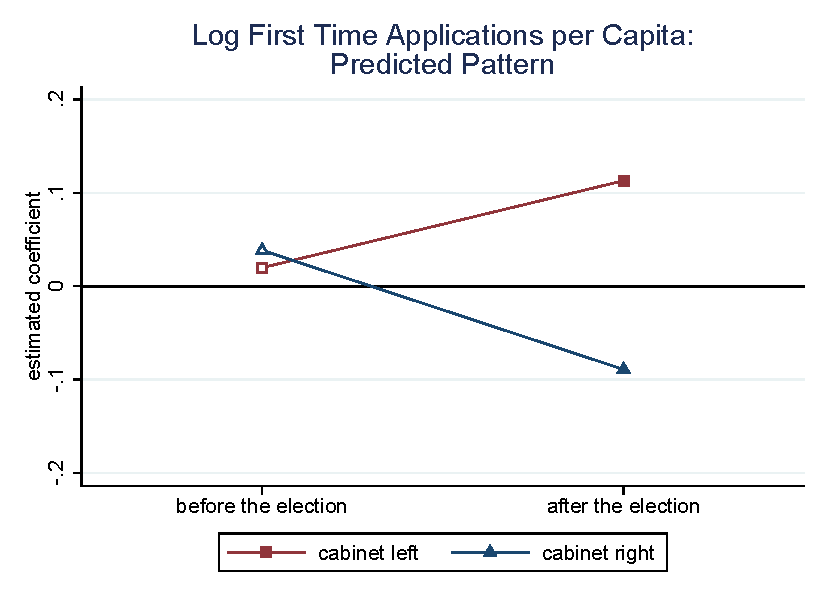
\includegraphics[width=1\textwidth]{figures_edited/app_graph1_baseline.pdf}
	\caption{log First Time Asylum Applications per Capita: Predicted Pattern}
\end{figure}

\begin{table}[!ht]\centering
\renewcommand{\arraystretch}{1.25}
\def\sym#1{\ifmmode^{#1}\else\(^{#1}\)\fi}
\caption{Log First Time Applications per Capita: Predicted Pattern}
\begin{tabular}[]{l*{2}{c}}
	\hline\hline
	                    &\multicolumn{1}{c}{(1)}&\multicolumn{1}{c}{(2)}\\
                    &\multicolumn{1}{c}{left}&\multicolumn{1}{c}{right}\\
\hline
before              &      0.0199         &      0.0385         \\
                    &    (0.0296)         &    (0.0231)         \\
after               &       0.113\sym{***}&     -0.0891\sym{***}\\
                    &    (0.0227)         &    (0.0237)         \\
\hline
Observations        &       23248         &       23248         \\

	\hline\hline
	\multicolumn{3}{c}{\footnotesize Standard errors in parentheses} \\
	\multicolumn{3}{c}{\footnotesize (\sym{*} \(p<0.05\), \sym{**} \(p<0.01\), \sym{***} \(p<0.001\))}\\
\end{tabular}
\end{table}

\clearpage
\textbf{Baseline Specification - Model 2}
\begin{table}[!ht]\centering
	\scriptsize
	\renewcommand{\arraystretch}{1.1}
	\def\sym#1{\ifmmode^{#1}\else\(^{#1}\)\fi}
	\caption{Determinants of log(First time asylum applications per capita)}
	\begin{tabular}{l*{3}{c}}
		\hline\hline
		                    &\multicolumn{1}{c}{(1)}         &\multicolumn{1}{c}{(2)}         &\multicolumn{1}{c}{(3)}         \\
\hline
Political Terror Scale&       0.407\sym{***}&       0.407\sym{***}&                     \\
                    &    (0.0712)         &    (0.0707)         &                     \\
Civic Liberty (FHI) &       0.189         &       0.188         &                     \\
                    &     (0.140)         &     (0.138)         &                     \\
Political Rights (FHI)&      0.0408         &      0.0429         &                     \\
                    &    (0.0759)         &    (0.0759)         &                     \\
Quarterly civil war battle death (000s)&       0.188\sym{***}&       0.186\sym{***}&                     \\
                    &    (0.0238)         &    (0.0236)         &                     \\
Log origin country real GDP per capita&      -0.655\sym{***}&      -0.656\sym{***}&                     \\
                    &     (0.165)         &     (0.163)         &                     \\
Log destination country real GDP per capita&      -1.475\sym{**} &      -1.555\sym{***}&      -1.211\sym{*}  \\
                    &     (0.490)         &     (0.440)         &     (0.465)         \\
Quarterly unemployment rate at destination&     -0.0732\sym{***}&     -0.0744\sym{***}&     -0.0713\sym{***}\\
                    &    (0.0117)         &    (0.0111)         &    (0.0120)         \\
Cabinet position left * 6 quarters before the election&      0.0634         &      0.0580         &      0.0507         \\
                    &    (0.0411)         &    (0.0388)         &    (0.0420)         \\
Cabinet position left * 5 quarters before the election&     -0.0149         &     -0.0165         &     -0.0223         \\
                    &    (0.0391)         &    (0.0391)         &    (0.0398)         \\
Cabinet position left * 4 quarters before the election&      0.0442         &      0.0432         &      0.0370         \\
                    &    (0.0384)         &    (0.0397)         &    (0.0398)         \\
Cabinet position left * 3 quarters before the election&      0.0516         &      0.0515         &      0.0367         \\
                    &    (0.0435)         &    (0.0428)         &    (0.0458)         \\
Cabinet position left * 2 quarters before the election&      0.0251         &      0.0230         &    -0.00134         \\
                    &    (0.0338)         &    (0.0344)         &    (0.0351)         \\
Cabinet position left * 1 quarters before the election&      0.0158         &      0.0144         &   -0.000607         \\
                    &    (0.0382)         &    (0.0380)         &    (0.0386)         \\
Cabinet position left * election quarter&      0.0547         &      0.0512         &      0.0443         \\
                    &    (0.0390)         &    (0.0386)         &    (0.0401)         \\
Cabinet position left * 1 quarters after the election&       0.101\sym{*}  &      0.0944\sym{*}  &      0.0982\sym{*}  \\
                    &    (0.0412)         &    (0.0412)         &    (0.0425)         \\
Cabinet position left * 2 quarters after the election&      0.0928\sym{**} &      0.0883\sym{**} &      0.0838\sym{*}  \\
                    &    (0.0321)         &    (0.0313)         &    (0.0320)         \\
Cabinet position left * 3 quarters after the election&       0.104\sym{**} &      0.0941\sym{**} &       0.103\sym{**} \\
                    &    (0.0336)         &    (0.0328)         &    (0.0338)         \\
Cabinet position left * 4 quarters after the election&       0.161\sym{***}&       0.150\sym{***}&       0.153\sym{***}\\
                    &    (0.0300)         &    (0.0287)         &    (0.0307)         \\
Cabinet position left * 5 quarters after the election&       0.205\sym{***}&       0.195\sym{***}&       0.190\sym{***}\\
                    &    (0.0311)         &    (0.0286)         &    (0.0313)         \\
Cabinet position left * 6 quarters after the election&       0.116\sym{**} &       0.106\sym{**} &       0.110\sym{**} \\
                    &    (0.0343)         &    (0.0315)         &    (0.0344)         \\
Cabinet position right * 6 quarters before the election&      0.0449         &      0.0486         &      0.0471         \\
                    &    (0.0420)         &    (0.0414)         &    (0.0415)         \\
Cabinet position right * 5 quarters before the election&      0.0818\sym{*}  &      0.0859\sym{*}  &      0.0891\sym{**} \\
                    &    (0.0340)         &    (0.0327)         &    (0.0323)         \\
Cabinet position right * 4 quarters before the election&    -0.00316         &     0.00270         &  -0.0000381         \\
                    &    (0.0381)         &    (0.0377)         &    (0.0371)         \\
Cabinet position right * 3 quarters before the election&      0.0104         &      0.0174         &     0.00903         \\
                    &    (0.0310)         &    (0.0295)         &    (0.0308)         \\
Cabinet position right * 2 quarters before the election&      0.0632         &      0.0666         &      0.0627         \\
                    &    (0.0394)         &    (0.0386)         &    (0.0397)         \\
Cabinet position right * 1 quarters before the election&      0.0754\sym{*}  &      0.0727\sym{*}  &      0.0708\sym{*}  \\
                    &    (0.0350)         &    (0.0350)         &    (0.0346)         \\
Cabinet position right * election quarter&      0.0300         &      0.0299         &      0.0302         \\
                    &    (0.0386)         &    (0.0376)         &    (0.0382)         \\
Cabinet position right * 1 quarters after the election&     -0.0769\sym{*}  &     -0.0722\sym{*}  &     -0.0780\sym{*}  \\
                    &    (0.0320)         &    (0.0322)         &    (0.0313)         \\
Cabinet position right * 2 quarters after the election&      -0.136\sym{***}&      -0.131\sym{***}&      -0.142\sym{***}\\
                    &    (0.0370)         &    (0.0366)         &    (0.0383)         \\
Cabinet position right * 3 quarters after the election&      -0.132\sym{**} &      -0.126\sym{**} &      -0.133\sym{**} \\
                    &    (0.0406)         &    (0.0397)         &    (0.0388)         \\
Cabinet position right * 4 quarters after the election&     -0.0662         &     -0.0606         &     -0.0680         \\
                    &    (0.0360)         &    (0.0349)         &    (0.0368)         \\
Cabinet position right * 5 quarters after the election&     -0.0919\sym{*}  &     -0.0861\sym{*}  &     -0.0929\sym{*}  \\
                    &    (0.0359)         &    (0.0361)         &    (0.0358)         \\
Cabinet position right * 6 quarters after the election&    -0.00540         &     0.00115         &    -0.00750         \\
                    &    (0.0328)         &    (0.0301)         &    (0.0320)         \\
\hline
Observations        &       23248         &       23248         &       23248         \\
Adjusted \(R^{2}\)  &       0.447         &       0.176         &       0.451         \\
Fixed Effects       &           O         &       D x O         &       O x T         \\
Destination dummies &         Yes         &          No         &         Yes         \\
Quarter-Year dummies&         Yes         &         Yes         &          No         \\

		\hline\hline
		\multicolumn{4}{c}{\footnotesize Standard errors in parentheses (\sym{*} \(p<0.05\), \sym{**} \(p<0.01\), \sym{***} \(p<0.001\))}\\
	\end{tabular}
\end{table}


\clearpage
\textbf{Baseline Specification - Model 2}
\begin{figure}[!ht]
	\centering
	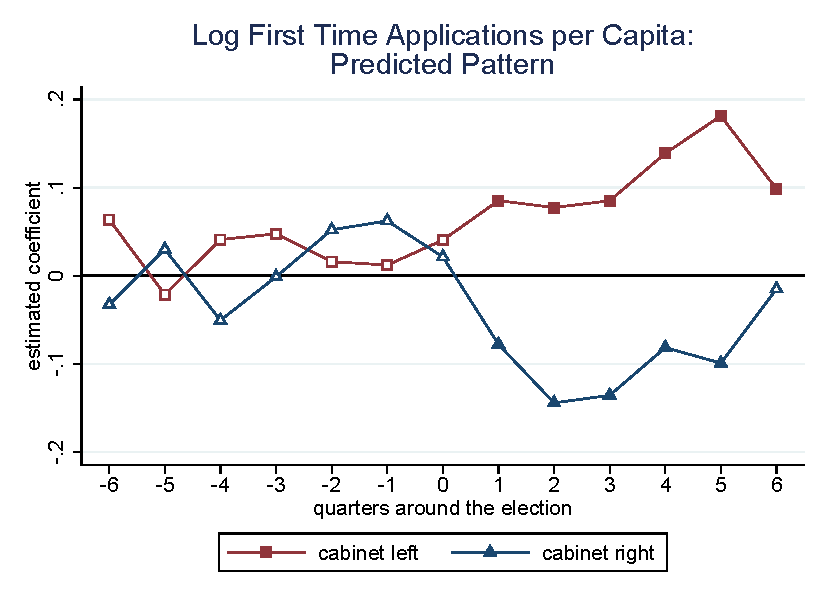
\includegraphics[width=0.7\textwidth]{figures_edited/app_graph2_baseline.pdf}
	\caption{log First Time Asylum Applications per Capita: Predicted Pattern}
\end{figure}

\begin{table}[!ht]\centering
	\footnotesize
	\renewcommand{\arraystretch}{1.2}
	\def\sym#1{\ifmmode^{#1}\else\(^{#1}\)\fi}
	\caption{Log First Time Applications per Capita: Predicted Pattern}
	\begin{tabular}{l*{2}{c}}
		\hline\hline
		                    &\multicolumn{1}{c}{(1)}&\multicolumn{1}{c}{(2)}\\
                    &\multicolumn{1}{c}{left}&\multicolumn{1}{c}{right}\\
\hline
 6 quarters before the election&      0.0580         &      0.0486         \\
                    &    (0.0388)         &    (0.0414)         \\
 5 quarters before the election&     -0.0165         &      0.0859\sym{**} \\
                    &    (0.0391)         &    (0.0327)         \\
 4 quarters before the election&      0.0432         &     0.00270         \\
                    &    (0.0397)         &    (0.0377)         \\
 3 quarters before the election&      0.0515         &      0.0174         \\
                    &    (0.0428)         &    (0.0295)         \\
 2 quarters before the election&      0.0230         &      0.0666         \\
                    &    (0.0344)         &    (0.0386)         \\
 1 quarters before the election&      0.0144         &      0.0727\sym{*}  \\
                    &    (0.0380)         &    (0.0350)         \\
Quarter of the election&      0.0512         &      0.0299         \\
                    &    (0.0386)         &    (0.0376)         \\
 1 quarters after the election&      0.0944\sym{*}  &     -0.0722\sym{*}  \\
                    &    (0.0412)         &    (0.0322)         \\
 2 quarters after the election&      0.0883\sym{**} &      -0.131\sym{***}\\
                    &    (0.0313)         &    (0.0366)         \\
 3 quarters after the election&      0.0941\sym{**} &      -0.126\sym{**} \\
                    &    (0.0328)         &    (0.0397)         \\
 4 quarters after the election&       0.150\sym{***}&     -0.0606         \\
                    &    (0.0287)         &    (0.0349)         \\
 5 quarters after the election&       0.195\sym{***}&     -0.0861\sym{*}  \\
                    &    (0.0286)         &    (0.0361)         \\
 6 quarters after the election&       0.106\sym{***}&     0.00115         \\
                    &    (0.0315)         &    (0.0301)         \\
\hline
Observations        &       23248         &       23248         \\

		\hline\hline
		\multicolumn{3}{c}{\footnotesize Standard errors in parentheses} \\
		\multicolumn{3}{c}{\footnotesize (\sym{*} \(p<0.05\), \sym{**} \(p<0.01\), \sym{***} \(p<0.001\))}\\
	\end{tabular}
\end{table}

% ===============================================================================================================


\FloatBarrier
\clearpage
\section{Robustness}

\subsection{Use destination, origin and time fixed effects}
\textbf{ R1: Use destination, origin and time fixed effects - Model 1}

\begin{figure}[!ht]
	\centering
	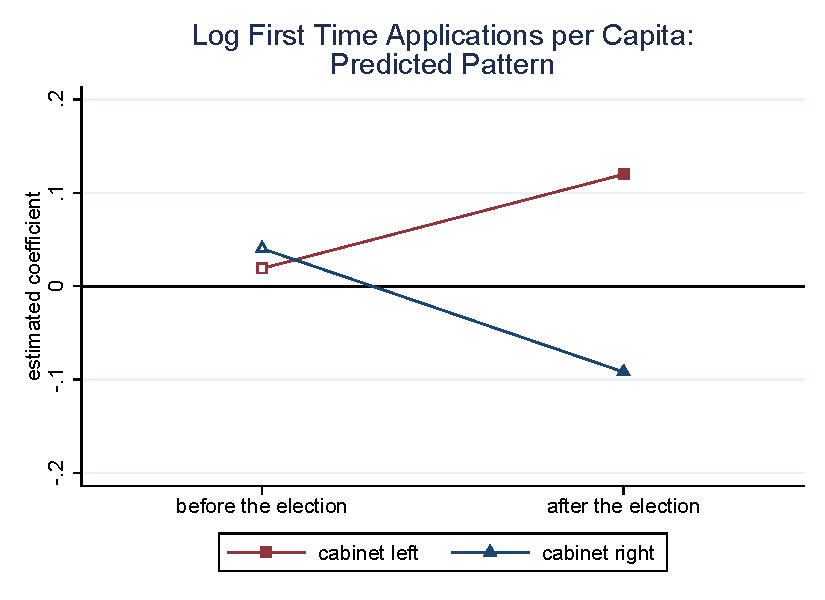
\includegraphics[width=1\textwidth]{figures_edited/app_graph1_R1.pdf}
	\caption{R1: log First Time Asylum Applications per Capita: Predicted Pattern}
\end{figure}

\begin{table}[!ht]\centering
	\renewcommand{\arraystretch}{1.25}
	\def\sym#1{\ifmmode^{#1}\else\(^{#1}\)\fi}
	\caption{R1: Log First Time Applications per Capita: Predicted Pattern}
	\begin{tabular}{l*{2}{c}}
		\hline\hline
		                    &\multicolumn{1}{c}{(1)}&\multicolumn{1}{c}{(2)}\\
                    &\multicolumn{1}{c}{left}&\multicolumn{1}{c}{right}\\
\hline
before              &      0.0190         &      0.0403         \\
                    &    (0.0297)         &    (0.0230)         \\
after               &       0.120\sym{***}&     -0.0912\sym{***}\\
                    &    (0.0236)         &    (0.0246)         \\
\hline
Observations        &       23248         &       23248         \\

		\hline\hline
		\multicolumn{3}{c}{\footnotesize Standard errors in parentheses} \\
		\multicolumn{3}{c}{\footnotesize (\sym{*} \(p<0.05\), \sym{**} \(p<0.01\), \sym{***} \(p<0.001\))}\\
	\end{tabular}
\end{table}

\clearpage
\textbf{ R1: Use destination, origin and time fixed effects - Model 2}
\begin{figure}[!ht]
	\centering
	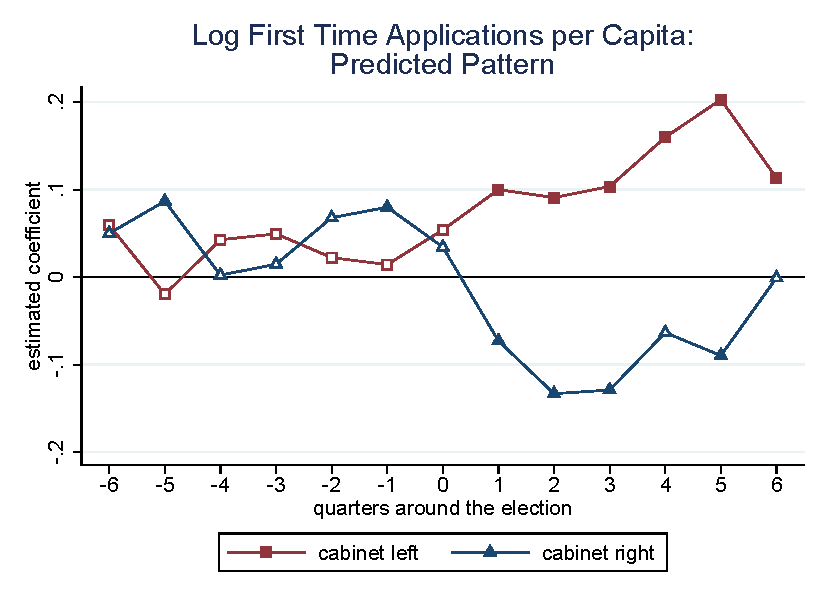
\includegraphics[width=0.7\textwidth]{figures_edited/app_graph2_R1.pdf}
	\caption{R1: log First Time Asylum Applications per Capita: Predicted Pattern}
\end{figure}

\begin{table}[!ht]\centering
	\footnotesize
	\renewcommand{\arraystretch}{1.2}
	\def\sym#1{\ifmmode^{#1}\else\(^{#1}\)\fi}
	\caption{R1: Log First Time Applications per Capita: Predicted Pattern}
	\begin{tabular}{l*{2}{c}}
		\hline\hline
		                    &\multicolumn{1}{c}{(1)}&\multicolumn{1}{c}{(2)}\\
                    &\multicolumn{1}{c}{left}&\multicolumn{1}{c}{right}\\
\hline
 6 quarters before the election&      0.0594         &      0.0500         \\
                    &    (0.0394)         &    (0.0410)         \\
 5 quarters before the election&     -0.0196         &      0.0868\sym{**} \\
                    &    (0.0391)         &    (0.0321)         \\
 4 quarters before the election&      0.0427         &     0.00226         \\
                    &    (0.0398)         &    (0.0376)         \\
 3 quarters before the election&      0.0494         &      0.0147         \\
                    &    (0.0431)         &    (0.0299)         \\
 2 quarters before the election&      0.0223         &      0.0679         \\
                    &    (0.0352)         &    (0.0384)         \\
 1 quarters before the election&      0.0143         &      0.0799\sym{*}  \\
                    &    (0.0379)         &    (0.0350)         \\
Quarter of the election&      0.0540         &      0.0343         \\
                    &    (0.0381)         &    (0.0378)         \\
 1 quarters after the election&       0.100\sym{*}  &     -0.0730\sym{*}  \\
                    &    (0.0411)         &    (0.0319)         \\
 2 quarters after the election&      0.0909\sym{**} &      -0.133\sym{***}\\
                    &    (0.0314)         &    (0.0366)         \\
 3 quarters after the election&       0.103\sym{**} &      -0.129\sym{**} \\
                    &    (0.0334)         &    (0.0404)         \\
 4 quarters after the election&       0.160\sym{***}&     -0.0634         \\
                    &    (0.0297)         &    (0.0358)         \\
 5 quarters after the election&       0.203\sym{***}&     -0.0897\sym{*}  \\
                    &    (0.0304)         &    (0.0362)         \\
 6 quarters after the election&       0.113\sym{***}&   -0.000866         \\
                    &    (0.0332)         &    (0.0317)         \\
\hline
Observations        &       23248         &       23248         \\

		\hline\hline
		\multicolumn{3}{c}{\footnotesize Standard errors in parentheses} \\
		\multicolumn{3}{c}{\footnotesize (\sym{*} \(p<0.05\), \sym{**} \(p<0.01\), \sym{***} \(p<0.001\))}\\
	\end{tabular}
\end{table}

% ===============================================================================================================

\FloatBarrier
\clearpage
\subsection{Use destination and origin*time fixed effects}
\textbf{R2: Use destination and origin*time fixed effects - Model 1}

\begin{figure}[!ht]
	\centering
	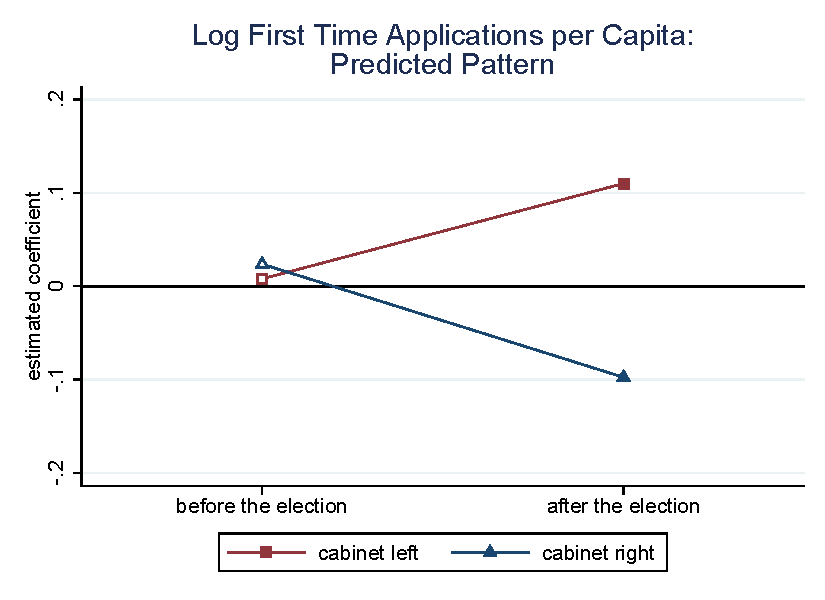
\includegraphics[width=1\textwidth]{figures_edited/app_graph1_R2.pdf}
	\caption{R2: log First Time Asylum Applications per Capita: Predicted Pattern}
\end{figure}

\begin{table}[!ht]\centering
	\renewcommand{\arraystretch}{1.25}
	\def\sym#1{\ifmmode^{#1}\else\(^{#1}\)\fi}
	\caption{R2: Log First Time Applications per Capita: Predicted Pattern}
	\begin{tabular}{l*{2}{c}}
		\hline\hline
		                    &\multicolumn{1}{c}{(1)}&\multicolumn{1}{c}{(2)}\\
                    &\multicolumn{1}{c}{left}&\multicolumn{1}{c}{right}\\
\hline
before              &     0.00604         &      0.0417         \\
                    &    (0.0309)         &    (0.0232)         \\
after               &       0.114\sym{***}&     -0.0929\sym{***}\\
                    &    (0.0238)         &    (0.0242)         \\
\hline
Observations        &       23248         &       23248         \\

		\hline\hline
		\multicolumn{3}{c}{\footnotesize Standard errors in parentheses} \\
		\multicolumn{3}{c}{\footnotesize (\sym{*} \(p<0.05\), \sym{**} \(p<0.01\), \sym{***} \(p<0.001\))}\\
	\end{tabular}
\end{table}

\clearpage
\textbf{R2: Use destination and origin*time fixed effects - Model 2}
\begin{figure}[!ht]
	\centering
	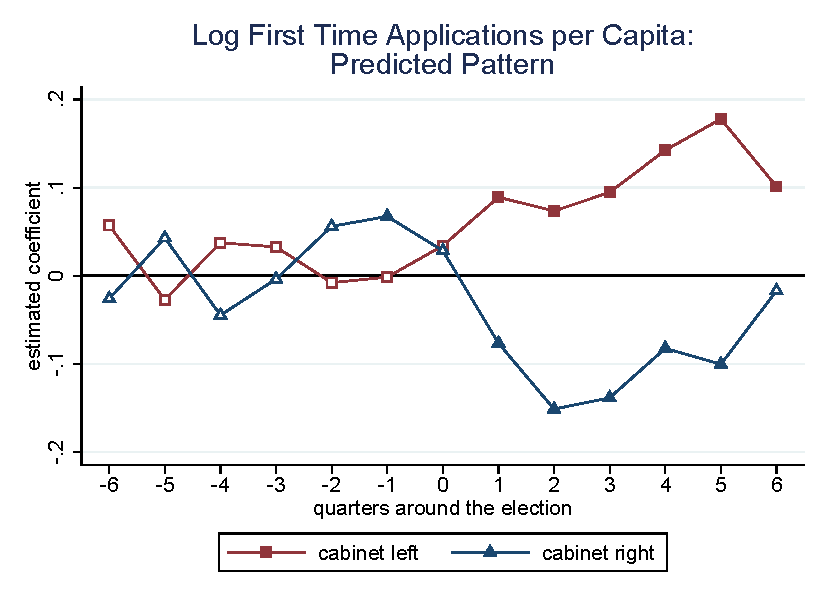
\includegraphics[width=0.7\textwidth]{figures_edited/app_graph2_R2.pdf}
	\caption{R2: log First Time Asylum Applications per Capita: Predicted Pattern}
\end{figure}

\begin{table}[!ht]\centering
	\footnotesize
	\renewcommand{\arraystretch}{1.2}
	\def\sym#1{\ifmmode^{#1}\else\(^{#1}\)\fi}
	\caption{R2: Log First Time Applications per Capita: Predicted Pattern}
	\begin{tabular}{l*{2}{c}}
		\hline\hline
		                    &\multicolumn{1}{c}{(1)}&\multicolumn{1}{c}{(2)}\\
                    &\multicolumn{1}{c}{left}&\multicolumn{1}{c}{right}\\
\hline
 6 quarters before the election&      0.0553         &       0.133\sym{***}\\
                    &    (0.0380)         &    (0.0379)         \\
 5 quarters before the election&     -0.0630         &       0.135\sym{***}\\
                    &    (0.0373)         &    (0.0373)         \\
 4 quarters before the election&     -0.0326         &      0.0727         \\
                    &    (0.0393)         &    (0.0393)         \\
 3 quarters before the election&      0.0300         &       0.138\sym{***}\\
                    &    (0.0442)         &    (0.0314)         \\
 2 quarters before the election&      0.0137         &       0.120\sym{***}\\
                    &    (0.0332)         &    (0.0344)         \\
 1 quarters before the election&     -0.0362         &       0.100\sym{**} \\
                    &    (0.0362)         &    (0.0323)         \\
Quarter of the election&    -0.00979         &      0.0518         \\
                    &    (0.0360)         &    (0.0334)         \\
 1 quarters after the election&       0.147\sym{***}&     -0.0318         \\
                    &    (0.0361)         &    (0.0311)         \\
 2 quarters after the election&       0.132\sym{***}&     -0.0873\sym{**} \\
                    &    (0.0258)         &    (0.0331)         \\
 3 quarters after the election&      0.0660\sym{*}  &      -0.129\sym{***}\\
                    &    (0.0294)         &    (0.0366)         \\
 4 quarters after the election&       0.140\sym{***}&     -0.0418         \\
                    &    (0.0253)         &    (0.0321)         \\
 5 quarters after the election&       0.223\sym{***}&     -0.0439         \\
                    &    (0.0279)         &    (0.0332)         \\
 6 quarters after the election&      0.0948\sym{***}&      0.0409         \\
                    &    (0.0267)         &    (0.0314)         \\
\hline
Observations        &       23248         &       23248         \\

		\hline\hline
		\multicolumn{3}{c}{\footnotesize Standard errors in parentheses} \\
		\multicolumn{3}{c}{\footnotesize (\sym{*} \(p<0.05\), \sym{**} \(p<0.01\), \sym{***} \(p<0.001\))}\\
	\end{tabular}
\end{table}


% ===============================================================================================================


\clearpage
\FloatBarrier
\subsection{Control for past asylum applications}
\begin{table}[!ht]\centering
	\renewcommand{\arraystretch}{1.25}
	\small
	\def\sym#1{\ifmmode^{#1}\else\(^{#1}\)\fi}
	\caption{R3: Determinants of log(First time asylum applications per capita)}
	\begin{tabular}{l*{3}{c}}
		\hline\hline
		                                        &\multicolumn{1}{c}{(1)}         &\multicolumn{1}{c}{(2)}         &\multicolumn{1}{c}{(3)}         \\
\hline
Political Terror Scale                  &     0.412\sym{***}&     0.412\sym{***}&                   \\
                                        &  (0.0743)         &  (0.0739)         &                   \\
Civic Liberty (FHI)                     &     0.182         &     0.181         &                   \\
                                        &   (0.137)         &   (0.135)         &                   \\
Political Rights (FHI)                  &    0.0333         &    0.0354         &                   \\
                                        &  (0.0744)         &  (0.0746)         &                   \\
Quarterly civil war battle death (000s) &     0.131\sym{***}&     0.130\sym{***}&                   \\
                                        &  (0.0144)         &  (0.0142)         &                   \\
Log origin country real GDP per capita  &    -0.619\sym{***}&    -0.619\sym{***}&                   \\
                                        &   (0.168)         &   (0.166)         &                   \\
Log migrant stock in 2000/1             &     0.263\sym{***}&                   &     0.263\sym{***}\\
                                        &  (0.0215)         &                   &  (0.0215)         \\
Log distance from origin to destination &    -0.550         &                   &    -0.555         \\
                                        &   (0.295)         &                   &   (0.294)         \\
Log destination country real GDP per capita&    -1.486\sym{**} &    -1.590\sym{***}&    -1.295\sym{**} \\
                                        &   (0.503)         &   (0.446)         &   (0.477)         \\
Quarterly unemployment rate at destination&   -0.0469\sym{***}&   -0.0481\sym{***}&   -0.0462\sym{***}\\
                                        &  (0.0102)         & (0.00996)         &  (0.0102)         \\
Log average past asylum applications at destination&     0.638\sym{***}&     0.639\sym{***}&     0.621\sym{***}\\
                                        &  (0.0695)         &  (0.0598)         &  (0.0733)         \\
Cabinet position left * Before the election&   -0.0182         &   -0.0197         &   -0.0307         \\
                                        &  (0.0280)         &  (0.0284)         &  (0.0293)         \\
Cabinet position left * After the election&    0.0934\sym{***}&    0.0855\sym{***}&    0.0880\sym{***}\\
                                        &  (0.0225)         &  (0.0211)         &  (0.0227)         \\
Cabinet position right * Before the election&  -0.00112         &   0.00203         &   0.00221         \\
                                        &  (0.0249)         &  (0.0231)         &  (0.0245)         \\
Cabinet position right * After the election&    -0.125\sym{***}&    -0.119\sym{***}&    -0.125\sym{***}\\
                                        &  (0.0253)         &  (0.0240)         &  (0.0248)         \\
\hline
Observations                            &     23248         &     23248         &     23248         \\
Adjusted \(R^{2}\)                      &     0.459         &     0.211         &     0.464         \\
Fixed Effects                           &         O         &     D x O         &     O x T         \\
Destination dummies                     &       Yes         &        No         &       Yes         \\
Quarter-Year dummies                    &       Yes         &       Yes         &        No         \\

		\hline\hline
		\multicolumn{4}{l}{\footnotesize Standard errors in parentheses (\sym{*} \(p<0.05\), \sym{**} \(p<0.01\), \sym{***} \(p<0.001\))}\\
	\end{tabular}
\end{table}

\clearpage
\textbf{R3: Control for past asylum applications - Model 1}
\begin{figure}[!ht]
	\centering
	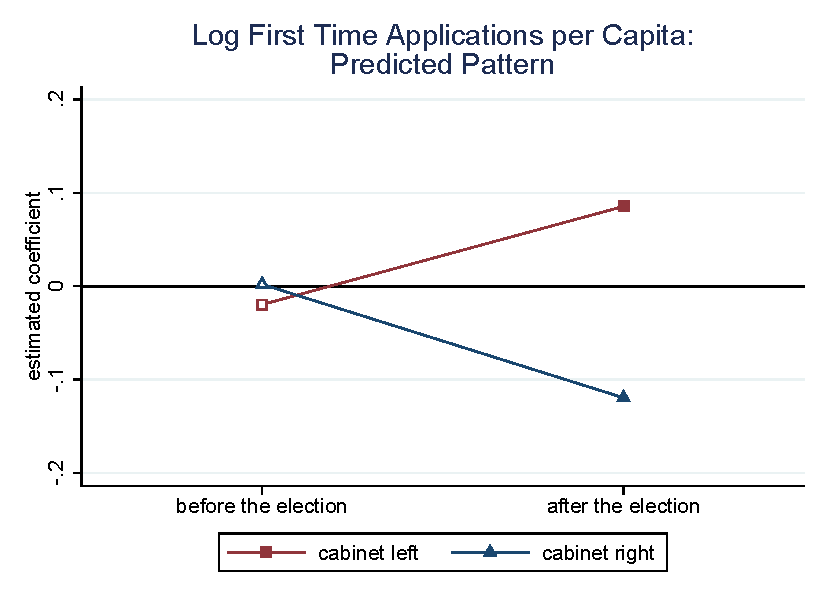
\includegraphics[width=1\textwidth]{figures_edited/app_graph1_R3.pdf}
	\caption{R3: log First Time Asylum Applications per Capita: Predicted Pattern}
\end{figure}

\begin{table}[!ht]\centering
	\renewcommand{\arraystretch}{1.25}
	\def\sym#1{\ifmmode^{#1}\else\(^{#1}\)\fi}
	\caption{R3: Log First Time Applications per Capita: Predicted Pattern}
	\begin{tabular}{l*{2}{c}}
		\hline\hline
		                    &\multicolumn{1}{c}{(1)}&\multicolumn{1}{c}{(2)}\\
                    &\multicolumn{1}{c}{left}&\multicolumn{1}{c}{right}\\
\hline
before              &     -0.0196         &     0.00209         \\
                    &    (0.0285)         &    (0.0231)         \\
after               &      0.0855\sym{***}&      -0.120\sym{***}\\
                    &    (0.0211)         &    (0.0239)         \\
\hline
Observations        &       23248         &       23248         \\

		\hline\hline
		\multicolumn{3}{c}{\footnotesize Standard errors in parentheses} \\
	    \multicolumn{3}{c}{\footnotesize (\sym{*} \(p<0.05\), \sym{**} \(p<0.01\), \sym{***} \(p<0.001\))}\\
	\end{tabular}
\end{table}

\clearpage
\textbf{R3: Control for past asylum applications - Model 2}
\begin{figure}[!ht]
	\centering
	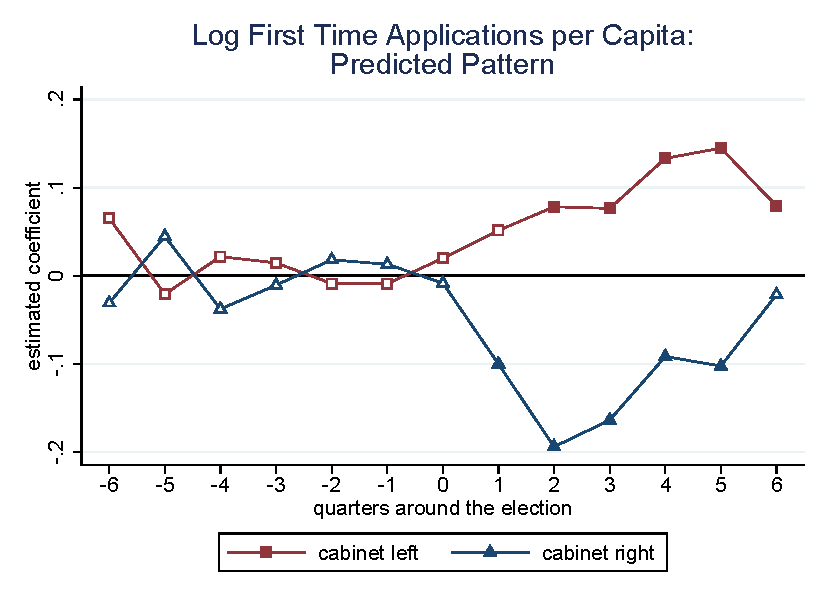
\includegraphics[width=0.7\textwidth]{figures_edited/app_graph2_R3.pdf}
	\caption{R3: log First Time Asylum Applications per Capita: Predicted Pattern}
\end{figure}

\begin{table}[!ht]\centering
	\footnotesize
	\renewcommand{\arraystretch}{1.2}
	\def\sym#1{\ifmmode^{#1}\else\(^{#1}\)\fi}
	\caption{R3: Log First Time Applications per Capita: Predicted Pattern}
	\begin{tabular}{l*{2}{c}}
		\hline\hline
		                    &\multicolumn{1}{c}{(1)}&\multicolumn{1}{c}{(2)}\\
                    &\multicolumn{1}{c}{left}&\multicolumn{1}{c}{right}\\
\hline
 6 quarters before the election&      0.0204         &    0.000299         \\
                    &    (0.0384)         &    (0.0411)         \\
 5 quarters before the election&     -0.0554         &      0.0542         \\
                    &    (0.0389)         &    (0.0329)         \\
 4 quarters before the election&     -0.0140         &     -0.0322         \\
                    &    (0.0388)         &    (0.0372)         \\
 3 quarters before the election&     -0.0122         &    -0.00977         \\
                    &    (0.0412)         &    (0.0294)         \\
 2 quarters before the election&     -0.0268         &      0.0152         \\
                    &    (0.0337)         &    (0.0375)         \\
 1 quarters before the election&     -0.0260         &     0.00784         \\
                    &    (0.0372)         &    (0.0357)         \\
Quarter of the election&      0.0116         &     -0.0148         \\
                    &    (0.0368)         &    (0.0382)         \\
 1 quarters after the election&      0.0413         &      -0.112\sym{***}\\
                    &    (0.0392)         &    (0.0325)         \\
 2 quarters after the election&      0.0693\sym{*}  &      -0.199\sym{***}\\
                    &    (0.0298)         &    (0.0361)         \\
 3 quarters after the election&      0.0657\sym{*}  &      -0.172\sym{***}\\
                    &    (0.0318)         &    (0.0402)         \\
 4 quarters after the election&       0.127\sym{***}&     -0.0870\sym{*}  \\
                    &    (0.0274)         &    (0.0348)         \\
 5 quarters after the election&       0.140\sym{***}&      -0.106\sym{**} \\
                    &    (0.0268)         &    (0.0363)         \\
 6 quarters after the election&      0.0711\sym{*}  &     -0.0221         \\
                    &    (0.0300)         &    (0.0300)         \\
\hline
Observations        &       23248         &       23248         \\

		\hline\hline
		\multicolumn{3}{c}{\footnotesize Standard errors in parentheses} \\
		\multicolumn{3}{c}{\footnotesize (\sym{*} \(p<0.05\), \sym{**} \(p<0.01\), \sym{***} \(p<0.001\))} \\
	\end{tabular}
\end{table}


% ===============================================================================================================


\clearpage
\FloatBarrier
\subsection{Include cabinet right dummy}
\begin{table}[!ht]\centering
	\renewcommand{\arraystretch}{1.25}
	\small
	\def\sym#1{\ifmmode^{#1}\else\(^{#1}\)\fi}
	\caption{R4: Determinants of log(First time asylum applications per capita)}
	\begin{tabular}{l*{3}{c}}
		\hline\hline
		                                        &\multicolumn{1}{c}{(1)}         &\multicolumn{1}{c}{(2)}         &\multicolumn{1}{c}{(3)}         \\
\hline
Political Terror Scale                  &     0.416\sym{***}&     0.416\sym{***}&                   \\
                                        &  (0.0711)         &  (0.0706)         &                   \\
Civic Liberty (FHI)                     &     0.191         &     0.190         &                   \\
                                        &   (0.138)         &   (0.136)         &                   \\
Political Rights (FHI)                  &    0.0370         &    0.0391         &                   \\
                                        &  (0.0756)         &  (0.0758)         &                   \\
Quarterly civil war battle death (000s) &     0.126\sym{***}&     0.125\sym{***}&                   \\
                                        &  (0.0141)         &  (0.0140)         &                   \\
Log origin country real GDP per capita  &    -0.648\sym{***}&    -0.650\sym{***}&                   \\
                                        &   (0.169)         &   (0.167)         &                   \\
Log migrant stock in 2000/1             &     0.264\sym{***}&                   &     0.263\sym{***}\\
                                        &  (0.0215)         &                   &  (0.0215)         \\
Log distance from origin to destination &    -0.547         &                   &    -0.552         \\
                                        &   (0.296)         &                   &   (0.295)         \\
Log destination country real GDP per capita&    -1.393\sym{**} &    -1.480\sym{**} &    -1.144\sym{*}  \\
                                        &   (0.492)         &   (0.446)         &   (0.466)         \\
Quarterly unemployment rate at destination&   -0.0729\sym{***}&   -0.0740\sym{***}&   -0.0710\sym{***}\\
                                        &  (0.0118)         &  (0.0111)         &  (0.0120)         \\
Weighted cabinet position right         &   -0.0587         &   -0.0441         &   -0.0481         \\
                                        &  (0.0499)         &  (0.0443)         &  (0.0511)         \\
Cabinet position left * Before the election&  -0.00571         & -0.000400         &   -0.0139         \\
                                        &  (0.0318)         &  (0.0318)         &  (0.0325)         \\
Cabinet position left * After the election&    0.0938\sym{***}&    0.0924\sym{***}&    0.0928\sym{***}\\
                                        &  (0.0228)         &  (0.0231)         &  (0.0234)         \\
Cabinet position right * Before the election&    0.0626\sym{*}  &    0.0585\sym{*}  &    0.0592\sym{*}  \\
                                        &  (0.0239)         &  (0.0234)         &  (0.0248)         \\
Cabinet position right * After the election&   -0.0666\sym{*}  &   -0.0678\sym{*}  &   -0.0734\sym{*}  \\
                                        &  (0.0284)         &  (0.0278)         &  (0.0275)         \\
\hline
Observations                            &     23248         &     23248         &     23248         \\
Adjusted \(R^{2}\)                      &     0.447         &     0.177         &     0.451         \\
Fixed Effects                           &         O         &     D x O         &     O x T         \\
Destination dummies                     &       Yes         &        No         &       Yes         \\
Quarter-Year dummies                    &       Yes         &       Yes         &        No         \\

		\hline\hline
		\multicolumn{4}{l}{\footnotesize Standard errors in parentheses (\sym{*} \(p<0.05\), \sym{**} \(p<0.01\), \sym{***} \(p<0.001\))}\\
	\end{tabular}
\end{table}

\clearpage
\textbf{R4: Include cabinet right dummy - Model 1}
\begin{figure}[!ht]
	\centering
	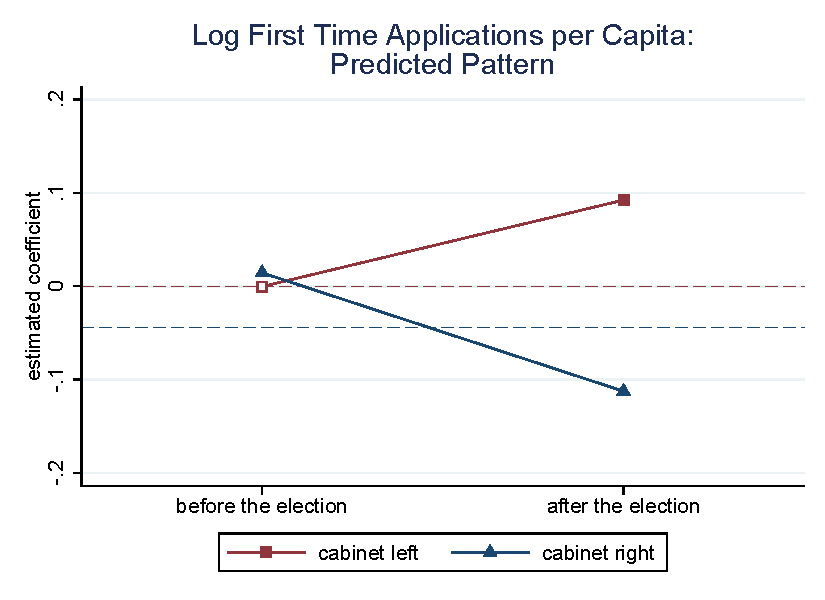
\includegraphics[width=1\textwidth]{figures_edited/app_graph1_R4.pdf}
	\caption{R4: log First Time Asylum Applications per Capita: Predicted Pattern}
\end{figure}

\begin{table}[!ht]\centering
	\renewcommand{\arraystretch}{1.25}
	\def\sym#1{\ifmmode^{#1}\else\(^{#1}\)\fi}
	\caption{R4: Log First Time Applications per Capita: Predicted Pattern}
	\begin{tabular}{l*{2}{c}}
		\hline\hline
		                    &\multicolumn{1}{c}{(1)}&\multicolumn{1}{c}{(2)}\\
                    &\multicolumn{1}{c}{left}&\multicolumn{1}{c}{right}\\
\hline
before              &   -0.000400         &      0.0585\sym{*}  \\
                    &    (0.0318)         &    (0.0234)         \\
after               &      0.0924\sym{***}&     -0.0678\sym{*}  \\
                    &    (0.0231)         &    (0.0278)         \\
\hline
Observations        &       23248         &       23248         \\

		\hline\hline
		\multicolumn{3}{c}{\footnotesize Standard errors in parentheses} \\
		\multicolumn{3}{c}{\footnotesize (\sym{*} \(p<0.05\), \sym{**} \(p<0.01\), \sym{***} \(p<0.001\))}\\
	\end{tabular}
\end{table}

\clearpage
\textbf{R4: Include cabinet right dummy - Model 2}
\begin{figure}[!ht]
	\centering
	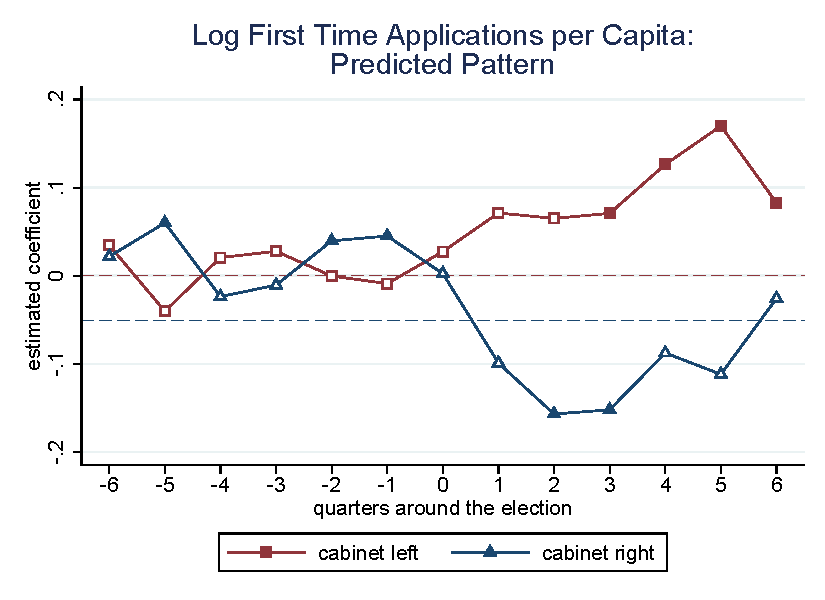
\includegraphics[width=0.7\textwidth]{figures_edited/app_graph2_R4.pdf}
	\caption{R4: log First Time Asylum Applications per Capita: Predicted Pattern}
\end{figure}

\begin{table}[!ht]\centering
	\footnotesize
	\renewcommand{\arraystretch}{1.2}
	\def\sym#1{\ifmmode^{#1}\else\(^{#1}\)\fi}
	\caption{R4: Log First Time Applications per Capita: Predicted Pattern}
	\begin{tabular}{l*{2}{c}}
		\hline\hline
		                    &\multicolumn{1}{c}{(1)}&\multicolumn{1}{c}{(2)}\\
                    &\multicolumn{1}{c}{left}&\multicolumn{1}{c}{right}\\
\hline
 6 quarters before the election&      0.0338         &      0.0718         \\
                    &    (0.0319)         &    (0.0390)         \\
 5 quarters before the election&     -0.0407         &       0.110\sym{***}\\
                    &    (0.0343)         &    (0.0294)         \\
 4 quarters before the election&      0.0203         &      0.0265         \\
                    &    (0.0421)         &    (0.0411)         \\
 3 quarters before the election&      0.0275         &      0.0398         \\
                    &    (0.0449)         &    (0.0314)         \\
 2 quarters before the election&   -0.000354         &      0.0902\sym{*}  \\
                    &    (0.0361)         &    (0.0396)         \\
 1 quarters before the election&    -0.00878         &      0.0956\sym{**} \\
                    &    (0.0443)         &    (0.0368)         \\
Quarter of the election&      0.0276         &      0.0528         \\
                    &    (0.0413)         &    (0.0359)         \\
 1 quarters after the election&      0.0711         &     -0.0484         \\
                    &    (0.0397)         &    (0.0365)         \\
 2 quarters after the election&      0.0647         &      -0.106\sym{**} \\
                    &    (0.0356)         &    (0.0357)         \\
 3 quarters after the election&      0.0705\sym{*}  &      -0.101\sym{*}  \\
                    &    (0.0336)         &    (0.0464)         \\
 4 quarters after the election&       0.126\sym{***}&     -0.0362         \\
                    &    (0.0317)         &    (0.0399)         \\
 5 quarters after the election&       0.170\sym{***}&     -0.0606         \\
                    &    (0.0279)         &    (0.0366)         \\
 6 quarters after the election&      0.0832\sym{**} &      0.0254         \\
                    &    (0.0277)         &    (0.0315)         \\
\hline
Observations        &       23248         &       23248         \\

		\hline\hline
		\multicolumn{3}{c}{\footnotesize Standard errors in parentheses} \\
		\multicolumn{3}{c}{\footnotesize (\sym{*} \(p<0.05\), \sym{**} \(p<0.01\), \sym{***} \(p<0.001\))} \\
	\end{tabular}
\end{table}


% ===============================================================================================================


\clearpage
\FloatBarrier
\subsection{Use log first time applications per capita in origin country as dependent variable}
\begin{table}[!ht]\centering
	\renewcommand{\arraystretch}{1.25}
	\small
	\def\sym#1{\ifmmode^{#1}\else\(^{#1}\)\fi}
	\caption{R5: Determinants of log(First time asylum applications per capita)}
	\begin{tabular}{l*{3}{c}}
		\hline\hline
		                                        &\multicolumn{1}{c}{(1)}         &\multicolumn{1}{c}{(2)}         &\multicolumn{1}{c}{(3)}         \\
\hline
Political Terror Scale                  &     0.406\sym{***}&     0.406\sym{***}&                   \\
                                        &  (0.0714)         &  (0.0709)         &                   \\
Civic Liberty (FHI)                     &     0.153         &     0.153         &                   \\
                                        &   (0.137)         &   (0.135)         &                   \\
Political Rights (FHI)                  &    0.0555         &    0.0576         &                   \\
                                        &  (0.0720)         &  (0.0720)         &                   \\
Quarterly civil war battle death (000s) &     0.193\sym{***}&     0.191\sym{***}&                   \\
                                        &  (0.0228)         &  (0.0227)         &                   \\
Log origin country real GDP per capita  &    -0.631\sym{***}&    -0.633\sym{***}&                   \\
                                        &   (0.161)         &   (0.159)         &                   \\
Log migrant stock in 2000/1             &     0.263\sym{***}&                   &     0.263\sym{***}\\
                                        &  (0.0215)         &                   &  (0.0214)         \\
Log distance from origin to destination &    -0.549         &                   &    -0.552         \\
                                        &   (0.296)         &                   &   (0.295)         \\
Log destination country real GDP per capita&    -1.449\sym{**} &    -1.527\sym{**} &    -1.239\sym{*}  \\
                                        &   (0.500)         &   (0.448)         &   (0.469)         \\
Quarterly unemployment rate at destination&   -0.0695\sym{***}&   -0.0707\sym{***}&   -0.0671\sym{***}\\
                                        &  (0.0117)         &  (0.0110)         &  (0.0119)         \\
Cabinet position left * Before the election&    0.0306         &    0.0290         &    0.0161         \\
                                        &  (0.0297)         &  (0.0298)         &  (0.0309)         \\
Cabinet position left * After the election&     0.126\sym{***}&     0.117\sym{***}&     0.119\sym{***}\\
                                        &  (0.0244)         &  (0.0227)         &  (0.0245)         \\
Cabinet position right * Before the election&    0.0325         &    0.0352         &    0.0335         \\
                                        &  (0.0242)         &  (0.0229)         &  (0.0242)         \\
Cabinet position right * After the election&   -0.0955\sym{***}&   -0.0898\sym{***}&   -0.0957\sym{***}\\
                                        &  (0.0247)         &  (0.0237)         &  (0.0246)         \\
\hline
Observations                            &     23248         &     23248         &     23248         \\
Adjusted \(R^{2}\)                      &     0.471         &     0.182         &     0.474         \\
Fixed Effects                           &         O         &     D x O         &     O x T         \\
Destination dummies                     &       Yes         &        No         &       Yes         \\
Quarter-Year dummies                    &       Yes         &       Yes         &        No         \\

		\hline\hline
		\multicolumn{4}{l}{\footnotesize Standard errors in parentheses (\sym{*} \(p<0.05\), \sym{**} \(p<0.01\), \sym{***} \(p<0.001\))}\\
	\end{tabular}
\end{table}

\clearpage
\textbf{R5: Use log first time applications per capita in origin country as dependent variable - Model 1}
\begin{figure}[!ht]
	\centering
	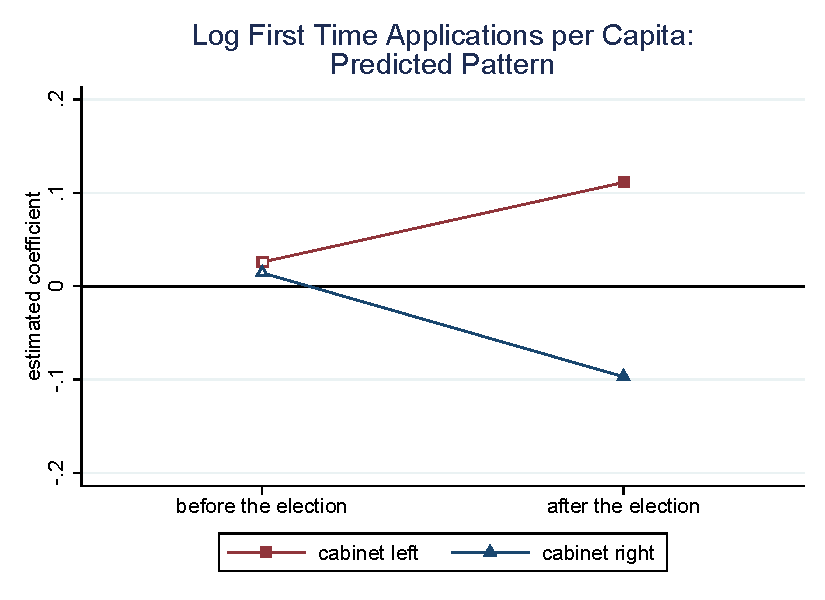
\includegraphics[width=1\textwidth]{figures_edited/app_graph1_R5.pdf}
	\caption{R5: log First Time Asylum Applications per Capita: Predicted Pattern}
\end{figure}

\begin{table}[!ht]\centering
	\renewcommand{\arraystretch}{1.25}
	\def\sym#1{\ifmmode^{#1}\else\(^{#1}\)\fi}
	\caption{R5: Log First Time Applications per Capita: Predicted Pattern}
	\begin{tabular}{l*{2}{c}}
		\hline\hline
		                    &\multicolumn{1}{c}{(1)}&\multicolumn{1}{c}{(2)}\\
                    &\multicolumn{1}{c}{left}&\multicolumn{1}{c}{right}\\
\hline
before              &      0.0290         &      0.0352         \\
                    &    (0.0298)         &    (0.0229)         \\
after               &       0.117\sym{***}&     -0.0898\sym{***}\\
                    &    (0.0227)         &    (0.0237)         \\
\hline
Observations        &       23248         &       23248         \\

		\hline\hline
		\multicolumn{3}{c}{\footnotesize Standard errors in parentheses} \\
		\multicolumn{3}{c}{\footnotesize (\sym{*} \(p<0.05\), \sym{**} \(p<0.01\), \sym{***} \(p<0.001\))}\\
	\end{tabular}
\end{table}

\clearpage
\textbf{R5: Use log first time applications per capita in origin country as dependent variable - Model 2}
\begin{figure}[!ht]
	\centering
	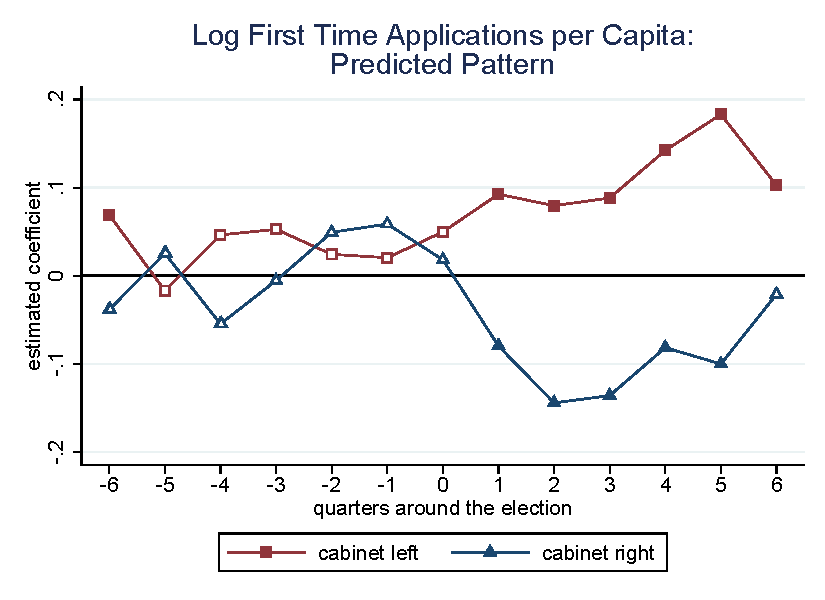
\includegraphics[width=0.7\textwidth]{figures_edited/app_graph2_R5.pdf}
	\caption{R5: log First Time Asylum Applications per Capita: Predicted Pattern}
\end{figure}

\begin{table}[!ht]\centering
	\footnotesize
	\renewcommand{\arraystretch}{1.2}
	\def\sym#1{\ifmmode^{#1}\else\(^{#1}\)\fi}
	\caption{R5: Log First Time Applications per Capita: Predicted Pattern}
	\begin{tabular}{l*{2}{c}}
		\hline\hline
		                    &\multicolumn{1}{c}{(1)}&\multicolumn{1}{c}{(2)}\\
                    &\multicolumn{1}{c}{left}&\multicolumn{1}{c}{right}\\
\hline
 6 quarters before the election&      0.0658         &      0.0433         \\
                    &    (0.0388)         &    (0.0414)         \\
 5 quarters before the election&    -0.00810         &      0.0815\sym{*}  \\
                    &    (0.0393)         &    (0.0326)         \\
 4 quarters before the election&      0.0524         &    -0.00134         \\
                    &    (0.0398)         &    (0.0376)         \\
 3 quarters before the election&      0.0599         &      0.0140         \\
                    &    (0.0427)         &    (0.0294)         \\
 2 quarters before the election&      0.0337         &      0.0646         \\
                    &    (0.0345)         &    (0.0386)         \\
 1 quarters before the election&      0.0238         &      0.0699\sym{*}  \\
                    &    (0.0381)         &    (0.0347)         \\
Quarter of the election&      0.0615         &      0.0274         \\
                    &    (0.0388)         &    (0.0375)         \\
 1 quarters after the election&       0.103\sym{*}  &     -0.0732\sym{*}  \\
                    &    (0.0411)         &    (0.0320)         \\
 2 quarters after the election&      0.0914\sym{**} &      -0.130\sym{***}\\
                    &    (0.0312)         &    (0.0365)         \\
 3 quarters after the election&      0.0984\sym{**} &      -0.125\sym{**} \\
                    &    (0.0328)         &    (0.0397)         \\
 4 quarters after the election&       0.155\sym{***}&     -0.0596         \\
                    &    (0.0287)         &    (0.0349)         \\
 5 quarters after the election&       0.197\sym{***}&     -0.0861\sym{*}  \\
                    &    (0.0286)         &    (0.0360)         \\
 6 quarters after the election&       0.111\sym{***}&    -0.00390         \\
                    &    (0.0314)         &    (0.0302)         \\
\hline
Observations        &       23248         &       23248         \\

		\hline\hline
		\multicolumn{3}{c}{\footnotesize Standard errors in parentheses} \\
		\multicolumn{3}{c}{\footnotesize (\sym{*} \(p<0.05\), \sym{**} \(p<0.01\), \sym{***} \(p<0.001\))} \\
	\end{tabular}
\end{table}



% ===============================================================================================================


\clearpage
\FloatBarrier
\subsection{Do not use lags for origin country variables}
\begin{table}[!ht]\centering
	\renewcommand{\arraystretch}{1.25}
	\small
	\def\sym#1{\ifmmode^{#1}\else\(^{#1}\)\fi}
	\caption{R6: Determinants of log(First time asylum applications per capita)}
	\begin{tabular}{l*{3}{c}}
		\hline\hline
		                                        &\multicolumn{1}{c}{(1)}         &\multicolumn{1}{c}{(2)}         &\multicolumn{1}{c}{(3)}         \\
\hline
Political Terror Scale                  &     0.343\sym{***}&     0.344\sym{***}&                   \\
                                        &  (0.0630)         &  (0.0625)         &                   \\
Civic Liberty (FHI)                     &     0.152         &     0.151         &                   \\
                                        &   (0.131)         &   (0.129)         &                   \\
Political Rights (FHI)                  &    0.0484         &    0.0510         &                   \\
                                        &  (0.0673)         &  (0.0675)         &                   \\
Quarterly civil war battle death (000s) &     0.160\sym{***}&     0.158\sym{***}&                   \\
                                        &  (0.0223)         &  (0.0221)         &                   \\
Log origin country real GDP per capita  &    -0.685\sym{***}&    -0.685\sym{***}&                   \\
                                        &   (0.150)         &   (0.148)         &                   \\
Log migrant stock in 2000/1             &     0.263\sym{***}&                   &     0.263\sym{***}\\
                                        &  (0.0215)         &                   &  (0.0214)         \\
Log distance from origin to destination &    -0.549         &                   &    -0.552         \\
                                        &   (0.296)         &                   &   (0.295)         \\
Log destination country real GDP per capita&    -1.412\sym{**} &    -1.488\sym{**} &    -1.175\sym{*}  \\
                                        &   (0.494)         &   (0.445)         &   (0.470)         \\
Quarterly unemployment rate at destination&   -0.0722\sym{***}&   -0.0733\sym{***}&   -0.0707\sym{***}\\
                                        &  (0.0117)         &  (0.0110)         &  (0.0119)         \\
Cabinet position left * Before the election&    0.0226         &    0.0211         &   0.00821         \\
                                        &  (0.0295)         &  (0.0296)         &  (0.0309)         \\
Cabinet position left * After the election&     0.122\sym{***}&     0.114\sym{***}&     0.115\sym{***}\\
                                        &  (0.0244)         &  (0.0228)         &  (0.0245)         \\
Cabinet position right * Before the election&    0.0366         &    0.0393         &    0.0372         \\
                                        &  (0.0244)         &  (0.0231)         &  (0.0243)         \\
Cabinet position right * After the election&   -0.0957\sym{***}&   -0.0900\sym{***}&   -0.0961\sym{***}\\
                                        &  (0.0247)         &  (0.0236)         &  (0.0246)         \\
\hline
Observations                            &     23248         &     23248         &     23248         \\
Adjusted \(R^{2}\)                      &     0.444         &     0.169         &     0.451         \\
Fixed Effects                           &         O         &     D x O         &     O x T         \\
Destination dummies                     &       Yes         &        No         &       Yes         \\
Quarter-Year dummies                    &       Yes         &       Yes         &        No         \\

		\hline\hline
		\multicolumn{4}{l}{\footnotesize Standard errors in parentheses (\sym{*} \(p<0.05\), \sym{**} \(p<0.01\), \sym{***} \(p<0.001\))}\\
	\end{tabular}
\end{table}

\clearpage
\textbf{R6: Do not use lags for origin country variables - Model 1}
\begin{figure}[!ht]
	\centering
	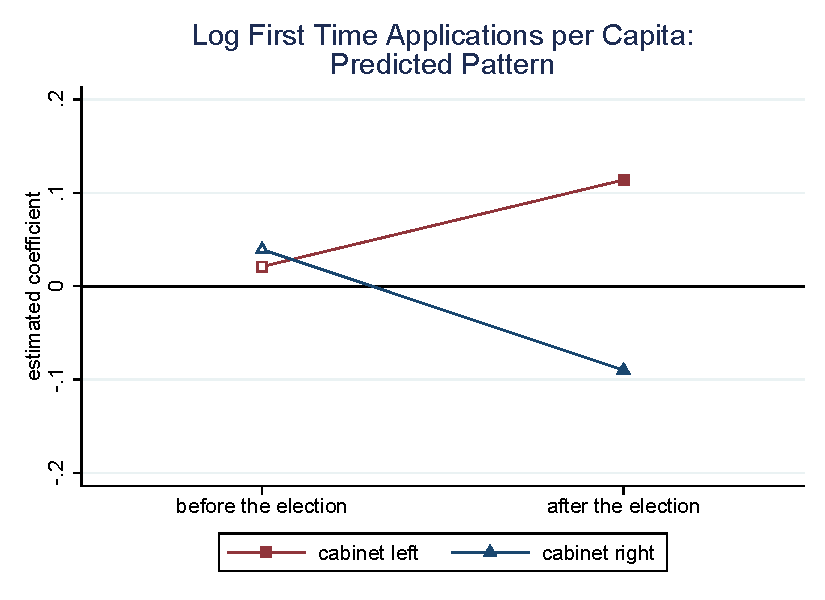
\includegraphics[width=1\textwidth]{figures_edited/app_graph1_R6.pdf}
	\caption{R6: log First Time Asylum Applications per Capita: Predicted Pattern}
\end{figure}

\begin{table}[!ht]\centering
	\renewcommand{\arraystretch}{1.25}
	\def\sym#1{\ifmmode^{#1}\else\(^{#1}\)\fi}
	\caption{R6: Log First Time Applications per Capita: Predicted Pattern}
	\begin{tabular}{l*{2}{c}}
		\hline\hline
		                    &\multicolumn{1}{c}{(1)}&\multicolumn{1}{c}{(2)}\\
                    &\multicolumn{1}{c}{left}&\multicolumn{1}{c}{right}\\
\hline
before              &      0.0211         &      0.0393         \\
                    &    (0.0296)         &    (0.0231)         \\
after               &       0.114\sym{***}&     -0.0900\sym{***}\\
                    &    (0.0228)         &    (0.0236)         \\
\hline
Observations        &       23248         &       23248         \\

		\hline\hline
		\multicolumn{3}{c}{\footnotesize Standard errors in parentheses} \\
		\multicolumn{3}{c}{\footnotesize (\sym{*} \(p<0.05\), \sym{**} \(p<0.01\), \sym{***} \(p<0.001\))}\\
	\end{tabular}
\end{table}

\clearpage
\textbf{R6: Do not use lags for origin country variables - Model 2}
\begin{figure}[!ht]
	\centering
	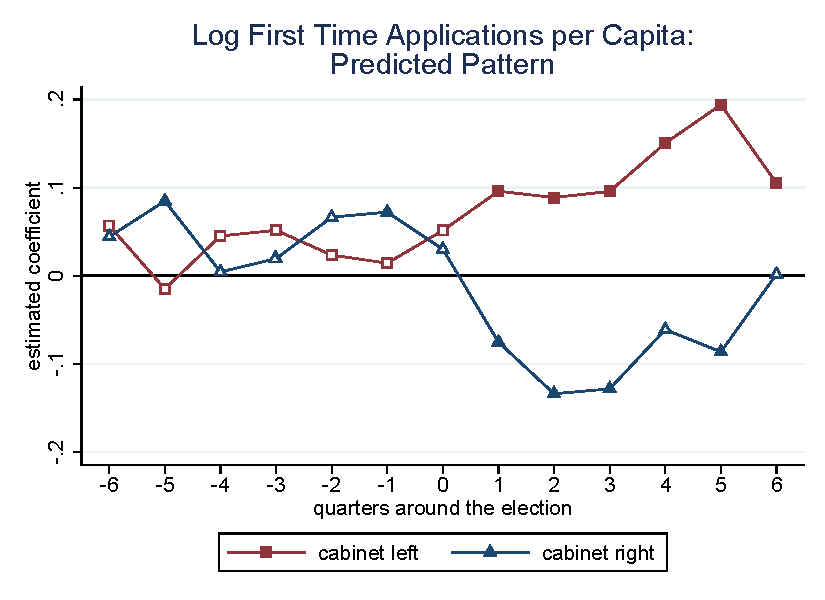
\includegraphics[width=0.7\textwidth]{figures_edited/app_graph2_R6.pdf}
	\caption{R6: log First Time Asylum Applications per Capita: Predicted Pattern}
\end{figure}

\begin{table}[!ht]\centering
	\footnotesize
	\renewcommand{\arraystretch}{1.2}
	\def\sym#1{\ifmmode^{#1}\else\(^{#1}\)\fi}
	\caption{R6: Log First Time Applications per Capita: Predicted Pattern}
	\begin{tabular}{l*{2}{c}}
		\hline\hline
		                    &\multicolumn{1}{c}{(1)}&\multicolumn{1}{c}{(2)}\\
                    &\multicolumn{1}{c}{left}&\multicolumn{1}{c}{right}\\
\hline
 6 quarters before the election&      0.0570         &      0.0444         \\
                    &    (0.0396)         &    (0.0413)         \\
 5 quarters before the election&     -0.0145         &      0.0854\sym{**} \\
                    &    (0.0395)         &    (0.0329)         \\
 4 quarters before the election&      0.0453         &     0.00466         \\
                    &    (0.0395)         &    (0.0378)         \\
 3 quarters before the election&      0.0520         &      0.0196         \\
                    &    (0.0428)         &    (0.0300)         \\
 2 quarters before the election&      0.0243         &      0.0678         \\
                    &    (0.0343)         &    (0.0383)         \\
 1 quarters before the election&      0.0151         &      0.0730\sym{*}  \\
                    &    (0.0381)         &    (0.0349)         \\
Quarter of the election&      0.0522         &      0.0304         \\
                    &    (0.0390)         &    (0.0378)         \\
 1 quarters after the election&      0.0958\sym{*}  &     -0.0745\sym{*}  \\
                    &    (0.0411)         &    (0.0320)         \\
 2 quarters after the election&      0.0892\sym{**} &      -0.133\sym{***}\\
                    &    (0.0317)         &    (0.0365)         \\
 3 quarters after the election&      0.0965\sym{**} &      -0.127\sym{**} \\
                    &    (0.0326)         &    (0.0397)         \\
 4 quarters after the election&       0.151\sym{***}&     -0.0597         \\
                    &    (0.0290)         &    (0.0348)         \\
 5 quarters after the election&       0.195\sym{***}&     -0.0862\sym{*}  \\
                    &    (0.0290)         &    (0.0356)         \\
 6 quarters after the election&       0.106\sym{***}&     0.00226         \\
                    &    (0.0318)         &    (0.0301)         \\
\hline
Observations        &       23248         &       23248         \\

		\hline\hline
		\multicolumn{3}{c}{\footnotesize Standard errors in parentheses} \\
		\multicolumn{3}{c}{\footnotesize (\sym{*} \(p<0.05\), \sym{**} \(p<0.01\), \sym{***} \(p<0.001\))} \\
	\end{tabular}
\end{table}


% ===============================================================================================================


\clearpage
\FloatBarrier
\subsection{Use Syrian battle death data from UCDP}
\begin{table}[!ht]\centering
	\renewcommand{\arraystretch}{1.25}
	\small
	\def\sym#1{\ifmmode^{#1}\else\(^{#1}\)\fi}
	\caption{R7: Determinants of log(First time asylum applications per capita)}
	\begin{tabular}{l*{3}{c}}
		\hline\hline
		                                        &\multicolumn{1}{c}{(1)}         &\multicolumn{1}{c}{(2)}         &\multicolumn{1}{c}{(3)}         \\
\hline
Political Terror Scale                  &     0.416\sym{***}&     0.416\sym{***}&                   \\
                                        &  (0.0712)         &  (0.0707)         &                   \\
Civic Liberty (FHI)                     &     0.191         &     0.190         &                   \\
                                        &   (0.138)         &   (0.136)         &                   \\
Political Rights (FHI)                  &    0.0369         &    0.0390         &                   \\
                                        &  (0.0756)         &  (0.0758)         &                   \\
Quarterly civil war battle death (000s) &     0.126\sym{***}&     0.125\sym{***}&                   \\
                                        &  (0.0141)         &  (0.0139)         &                   \\
Log origin country real GDP per capita  &    -0.649\sym{***}&    -0.650\sym{***}&                   \\
                                        &   (0.169)         &   (0.167)         &                   \\
Log migrant stock in 2000/1             &     0.264\sym{***}&                   &     0.263\sym{***}\\
                                        &  (0.0215)         &                   &  (0.0214)         \\
Log distance from origin to destination &    -0.547         &                   &    -0.552         \\
                                        &   (0.296)         &                   &   (0.295)         \\
Log destination country real GDP per capita&    -1.430\sym{**} &    -1.508\sym{**} &    -1.175\sym{*}  \\
                                        &   (0.496)         &   (0.446)         &   (0.470)         \\
Quarterly unemployment rate at destination&   -0.0726\sym{***}&   -0.0738\sym{***}&   -0.0707\sym{***}\\
                                        &  (0.0117)         &  (0.0110)         &  (0.0119)         \\
Cabinet position left * Before the election&    0.0213         &    0.0198         &   0.00821         \\
                                        &  (0.0295)         &  (0.0296)         &  (0.0309)         \\
Cabinet position left * After the election&     0.121\sym{***}&     0.113\sym{***}&     0.115\sym{***}\\
                                        &  (0.0243)         &  (0.0227)         &  (0.0245)         \\
Cabinet position right * Before the election&    0.0358         &    0.0384         &    0.0372         \\
                                        &  (0.0243)         &  (0.0231)         &  (0.0243)         \\
Cabinet position right * After the election&   -0.0942\sym{***}&   -0.0885\sym{***}&   -0.0961\sym{***}\\
                                        &  (0.0249)         &  (0.0238)         &  (0.0246)         \\
\hline
Observations                            &     23248         &     23248         &     23248         \\
Adjusted \(R^{2}\)                      &     0.447         &     0.177         &     0.451         \\
Fixed Effects                           &         O         &     D x O         &     O x T         \\
Destination dummies                     &       Yes         &        No         &       Yes         \\
Quarter-Year dummies                    &       Yes         &       Yes         &        No         \\

		\hline\hline
		\multicolumn{4}{l}{\footnotesize Standard errors in parentheses (\sym{*} \(p<0.05\), \sym{**} \(p<0.01\), \sym{***} \(p<0.001\))}\\
	\end{tabular}
\end{table}

\clearpage
\textbf{R7: Use Syrian battle death data from UCDP - Model 1}
\begin{figure}[!ht]
	\centering
	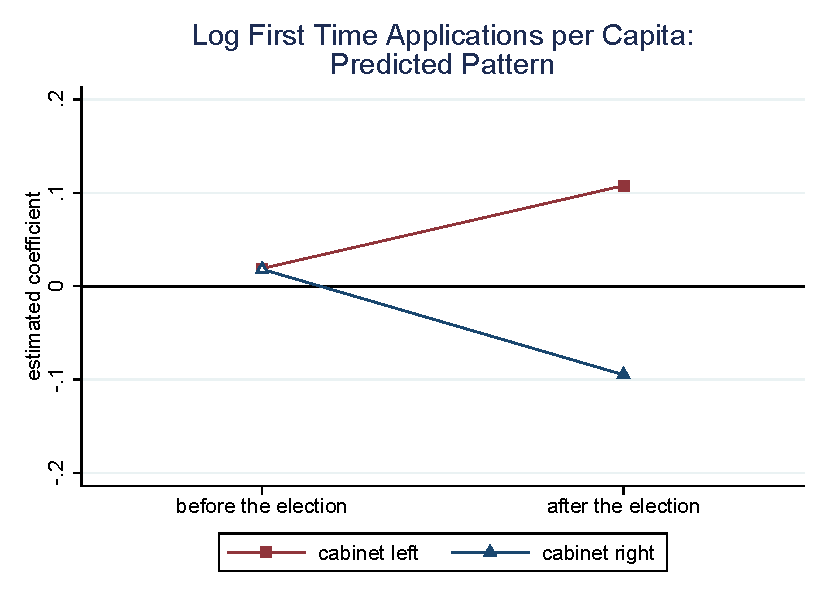
\includegraphics[width=1\textwidth]{figures_edited/app_graph1_R7.pdf}
	\caption{R7: log First Time Asylum Applications per Capita: Predicted Pattern}
\end{figure}

\begin{table}[!ht]\centering
	\renewcommand{\arraystretch}{1.25}
	\def\sym#1{\ifmmode^{#1}\else\(^{#1}\)\fi}
	\caption{R7: Log First Time Applications per Capita: Predicted Pattern}
	\begin{tabular}{l*{2}{c}}
		\hline\hline
		                    &\multicolumn{1}{c}{(1)}&\multicolumn{1}{c}{(2)}\\
                    &\multicolumn{1}{c}{left}&\multicolumn{1}{c}{right}\\
\hline
before              &      0.0199         &      0.0385         \\
                    &    (0.0296)         &    (0.0231)         \\
after               &       0.113\sym{***}&     -0.0891\sym{***}\\
                    &    (0.0227)         &    (0.0237)         \\
\hline
Observations        &       23248         &       23248         \\

		\hline\hline
		\multicolumn{3}{c}{\footnotesize Standard errors in parentheses} \\
		\multicolumn{3}{c}{\footnotesize (\sym{*} \(p<0.05\), \sym{**} \(p<0.01\), \sym{***} \(p<0.001\))}\\
	\end{tabular}
\end{table}

\clearpage
\textbf{R7: Use Syrian battle death data from UCDP - Model 2}
\begin{figure}[!ht]
	\centering
	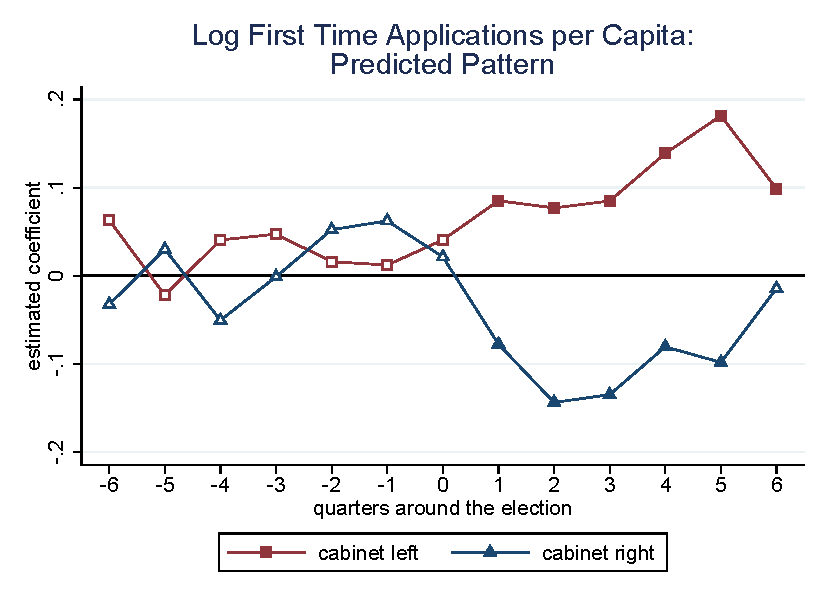
\includegraphics[width=0.7\textwidth]{figures_edited/app_graph2_R7.pdf}
	\caption{R7: log First Time Asylum Applications per Capita: Predicted Pattern}
\end{figure}

\begin{table}[!ht]\centering
	\footnotesize
	\renewcommand{\arraystretch}{1.2}
	\def\sym#1{\ifmmode^{#1}\else\(^{#1}\)\fi}
	\caption{R7: Log First Time Applications per Capita: Predicted Pattern}
	\begin{tabular}{l*{2}{c}}
		\hline\hline
		                    &\multicolumn{1}{c}{(1)}&\multicolumn{1}{c}{(2)}\\
                    &\multicolumn{1}{c}{left}&\multicolumn{1}{c}{right}\\
\hline
 6 quarters before the election&      0.0580         &      0.0486         \\
                    &    (0.0388)         &    (0.0414)         \\
 5 quarters before the election&     -0.0165         &      0.0859\sym{**} \\
                    &    (0.0391)         &    (0.0327)         \\
 4 quarters before the election&      0.0432         &     0.00270         \\
                    &    (0.0397)         &    (0.0377)         \\
 3 quarters before the election&      0.0515         &      0.0174         \\
                    &    (0.0428)         &    (0.0295)         \\
 2 quarters before the election&      0.0230         &      0.0666         \\
                    &    (0.0344)         &    (0.0386)         \\
 1 quarters before the election&      0.0144         &      0.0727\sym{*}  \\
                    &    (0.0380)         &    (0.0350)         \\
Quarter of the election&      0.0512         &      0.0299         \\
                    &    (0.0386)         &    (0.0376)         \\
 1 quarters after the election&      0.0944\sym{*}  &     -0.0722\sym{*}  \\
                    &    (0.0412)         &    (0.0322)         \\
 2 quarters after the election&      0.0883\sym{**} &      -0.131\sym{***}\\
                    &    (0.0313)         &    (0.0366)         \\
 3 quarters after the election&      0.0941\sym{**} &      -0.126\sym{**} \\
                    &    (0.0328)         &    (0.0397)         \\
 4 quarters after the election&       0.150\sym{***}&     -0.0606         \\
                    &    (0.0287)         &    (0.0349)         \\
 5 quarters after the election&       0.195\sym{***}&     -0.0861\sym{*}  \\
                    &    (0.0286)         &    (0.0361)         \\
 6 quarters after the election&       0.106\sym{***}&     0.00115         \\
                    &    (0.0315)         &    (0.0301)         \\
\hline
Observations        &       23248         &       23248         \\

		\hline\hline
		\multicolumn{3}{c}{\footnotesize Standard errors in parentheses} \\
		\multicolumn{3}{c}{\footnotesize (\sym{*} \(p<0.05\), \sym{**} \(p<0.01\), \sym{***} \(p<0.001\))} \\
	\end{tabular}
\end{table}


% ===============================================================================================================


\clearpage
\FloatBarrier
\subsection{Include a post 2007 dummy}
\begin{table}[!ht]\centering
	\renewcommand{\arraystretch}{1.25}
	\small
	\def\sym#1{\ifmmode^{#1}\else\(^{#1}\)\fi}
	\caption{R8: Determinants of log(First time asylum applications per capita)}
	\begin{tabular}{l*{2}{c}}
		\hline\hline
		                                        &\multicolumn{1}{c}{(1)}         &\multicolumn{1}{c}{(2)}         \\
\hline
Political Terror Scale                  &     0.407\sym{***}&     0.407\sym{***}\\
                                        &  (0.0712)         &  (0.0707)         \\
Civic Liberty (FHI)                     &     0.189         &     0.189         \\
                                        &   (0.140)         &   (0.138)         \\
Political Rights (FHI)                  &    0.0406         &    0.0427         \\
                                        &  (0.0758)         &  (0.0759)         \\
Quarterly civil war battle death (000s) &     0.188\sym{***}&     0.186\sym{***}\\
                                        &  (0.0238)         &  (0.0236)         \\
Log origin country real GDP per capita  &    -0.655\sym{***}&    -0.657\sym{***}\\
                                        &   (0.165)         &   (0.163)         \\
Log migrant stock in 2000/1             &     0.264\sym{***}&                   \\
                                        &  (0.0215)         &                   \\
Log distance from origin to destination &    -0.547         &                   \\
                                        &   (0.296)         &                   \\
Log destination country real GDP per capita&    -1.437\sym{**} &    -1.514\sym{**} \\
                                        &   (0.495)         &   (0.445)         \\
Quarterly unemployment rate at destination&   -0.0726\sym{***}&   -0.0738\sym{***}\\
                                        &  (0.0117)         &  (0.0110)         \\
after 2007                              &     0.208         &    -0.518\sym{**} \\
                                        &   (0.220)         &   (0.159)         \\
Cabinet position left * Before the election&    0.0214         &    0.0199         \\
                                        &  (0.0295)         &  (0.0296)         \\
Cabinet position left * After the election&     0.121\sym{***}&     0.113\sym{***}\\
                                        &  (0.0243)         &  (0.0227)         \\
Cabinet position right * Before the election&    0.0358         &    0.0385         \\
                                        &  (0.0243)         &  (0.0231)         \\
Cabinet position right * After the election&   -0.0949\sym{***}&   -0.0891\sym{***}\\
                                        &  (0.0248)         &  (0.0237)         \\
\hline
Observations                            &     23248         &     23248         \\
Adjusted \(R^{2}\)                      &     0.447         &     0.176         \\
Fixed Effects                           &         O         &     D x O         \\
Destination dummies                     &       Yes         &        No         \\
Quarter-Year dummies                    &       Yes         &       Yes         \\

		\hline\hline
		\multicolumn{3}{l}{\footnotesize Standard errors in parentheses (\sym{*} \(p<0.05\), \sym{**} \(p<0.01\), \sym{***} \(p<0.001\))}\\
	\end{tabular}
\end{table}

\clearpage
\textbf{R8: Include a post 2007 dummy - Model 1}
\begin{figure}[!ht]
	\centering
	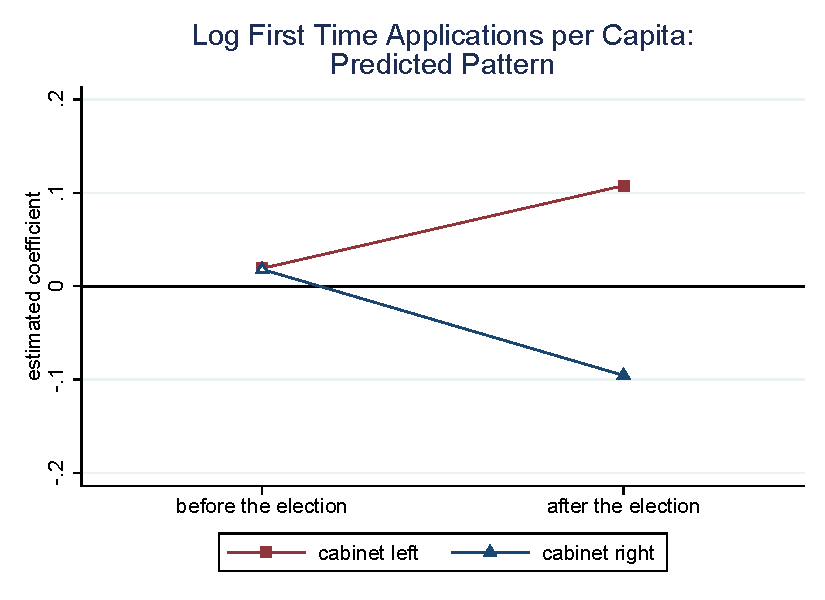
\includegraphics[width=1\textwidth]{figures_edited/app_graph1_R8.pdf}
	\caption{R8: log First Time Asylum Applications per Capita: Predicted Pattern}
\end{figure}

\begin{table}[!ht]\centering
	\renewcommand{\arraystretch}{1.25}
	\def\sym#1{\ifmmode^{#1}\else\(^{#1}\)\fi}
	\caption{R8: Log First Time Applications per Capita: Predicted Pattern}
	\begin{tabular}{l*{2}{c}}
		\hline\hline
		                    &\multicolumn{1}{c}{(1)}&\multicolumn{1}{c}{(2)}\\
                    &\multicolumn{1}{c}{left}&\multicolumn{1}{c}{right}\\
\hline
before              &      0.0199         &      0.0385         \\
                    &    (0.0296)         &    (0.0231)         \\
after               &       0.113\sym{***}&     -0.0891\sym{***}\\
                    &    (0.0227)         &    (0.0237)         \\
\hline
Observations        &       23248         &       23248         \\

		\hline\hline
		\multicolumn{3}{c}{\footnotesize Standard errors in parentheses} \\
		\multicolumn{3}{c}{\footnotesize (\sym{*} \(p<0.05\), \sym{**} \(p<0.01\), \sym{***} \(p<0.001\))}\\
	\end{tabular}
\end{table}

\clearpage
\textbf{R8: Include a post 2007 dummy - Model 2}
\begin{figure}[!ht]
	\centering
	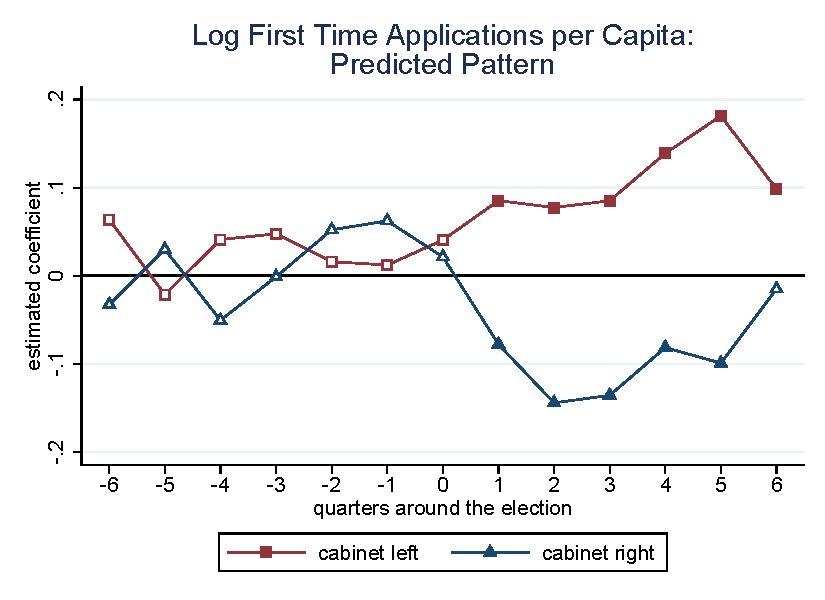
\includegraphics[width=0.7\textwidth]{figures_edited/app_graph2_R8.pdf}
	\caption{R8: log First Time Asylum Applications per Capita: Predicted Pattern}
\end{figure}

\begin{table}[!ht]\centering
	\footnotesize
	\renewcommand{\arraystretch}{1.2}
	\def\sym#1{\ifmmode^{#1}\else\(^{#1}\)\fi}
	\caption{R8: Log First Time Applications per Capita: Predicted Pattern}
	\begin{tabular}{l*{2}{c}}
		\hline\hline
		                    &\multicolumn{1}{c}{(1)}&\multicolumn{1}{c}{(2)}\\
                    &\multicolumn{1}{c}{left}&\multicolumn{1}{c}{right}\\
\hline
 6 quarters before the election&      0.0580         &      0.0486         \\
                    &    (0.0388)         &    (0.0414)         \\
 5 quarters before the election&     -0.0165         &      0.0859\sym{**} \\
                    &    (0.0391)         &    (0.0327)         \\
 4 quarters before the election&      0.0432         &     0.00270         \\
                    &    (0.0397)         &    (0.0377)         \\
 3 quarters before the election&      0.0515         &      0.0174         \\
                    &    (0.0428)         &    (0.0295)         \\
 2 quarters before the election&      0.0230         &      0.0666         \\
                    &    (0.0344)         &    (0.0386)         \\
 1 quarters before the election&      0.0144         &      0.0727\sym{*}  \\
                    &    (0.0380)         &    (0.0350)         \\
Quarter of the election&      0.0512         &      0.0299         \\
                    &    (0.0386)         &    (0.0376)         \\
 1 quarters after the election&      0.0944\sym{*}  &     -0.0722\sym{*}  \\
                    &    (0.0412)         &    (0.0322)         \\
 2 quarters after the election&      0.0883\sym{**} &      -0.131\sym{***}\\
                    &    (0.0313)         &    (0.0366)         \\
 3 quarters after the election&      0.0941\sym{**} &      -0.126\sym{**} \\
                    &    (0.0328)         &    (0.0397)         \\
 4 quarters after the election&       0.150\sym{***}&     -0.0606         \\
                    &    (0.0287)         &    (0.0349)         \\
 5 quarters after the election&       0.195\sym{***}&     -0.0861\sym{*}  \\
                    &    (0.0286)         &    (0.0361)         \\
 6 quarters after the election&       0.106\sym{***}&     0.00115         \\
                    &    (0.0315)         &    (0.0301)         \\
\hline
Observations        &       23248         &       23248         \\

		\hline\hline
		\multicolumn{3}{c}{\footnotesize Standard errors in parentheses} \\
		\multicolumn{3}{c}{\footnotesize (\sym{*} \(p<0.05\), \sym{**} \(p<0.01\), \sym{***} \(p<0.001\))} \\
	\end{tabular}
\end{table}


% ===============================================================================================================


\clearpage
\FloatBarrier
\subsection{Cluster standard errors on destination*origin level}
\textbf{R9: Cluster standard errors on destination*origin level - Model 1}
\begin{figure}[!ht]
	\centering
	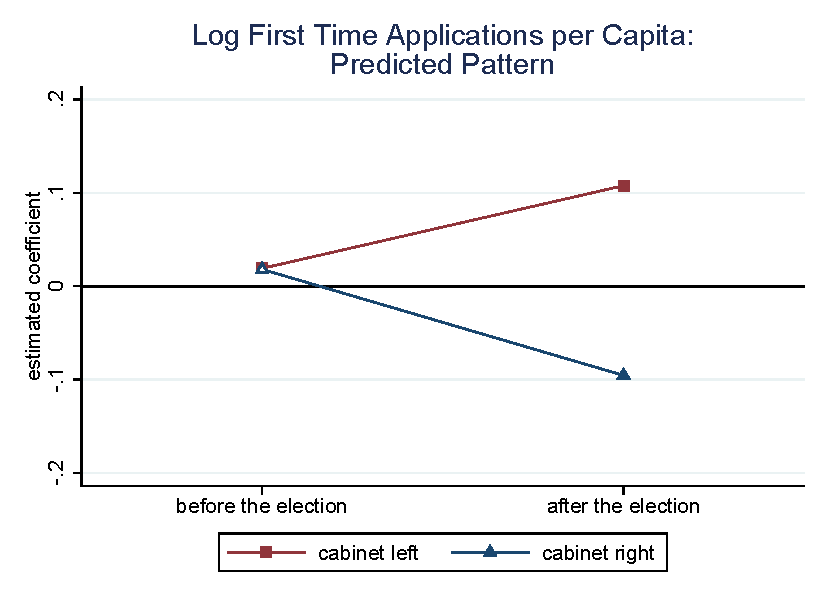
\includegraphics[width=1\textwidth]{figures_edited/app_graph1_R9.pdf}
	\caption{R9: log First Time Asylum Applications per Capita: Predicted Pattern}
\end{figure}

\begin{table}[!ht]\centering
	\renewcommand{\arraystretch}{1.25}
	\def\sym#1{\ifmmode^{#1}\else\(^{#1}\)\fi}
	\caption{R9: Log First Time Applications per Capita: Predicted Pattern}
	\begin{tabular}{l*{2}{c}}
		\hline\hline
		                    &\multicolumn{1}{c}{(1)}&\multicolumn{1}{c}{(2)}\\
                    &\multicolumn{1}{c}{left}&\multicolumn{1}{c}{right}\\
\hline
before              &      0.0198         &      0.0384         \\
                    &    (0.0326)         &    (0.0294)         \\
after               &       0.113\sym{***}&     -0.0885\sym{**} \\
                    &    (0.0285)         &    (0.0307)         \\
\hline
Observations        &       23248         &       23248         \\

		\hline\hline
		\multicolumn{3}{c}{\footnotesize Standard errors in parentheses} \\
		\multicolumn{3}{c}{\footnotesize (\sym{*} \(p<0.05\), \sym{**} \(p<0.01\), \sym{***} \(p<0.001\))}\\
	\end{tabular}
\end{table}

\clearpage
\textbf{R9: Cluster standard errors on destination*origin level - Model 2}
\begin{figure}[!ht]
	\centering
	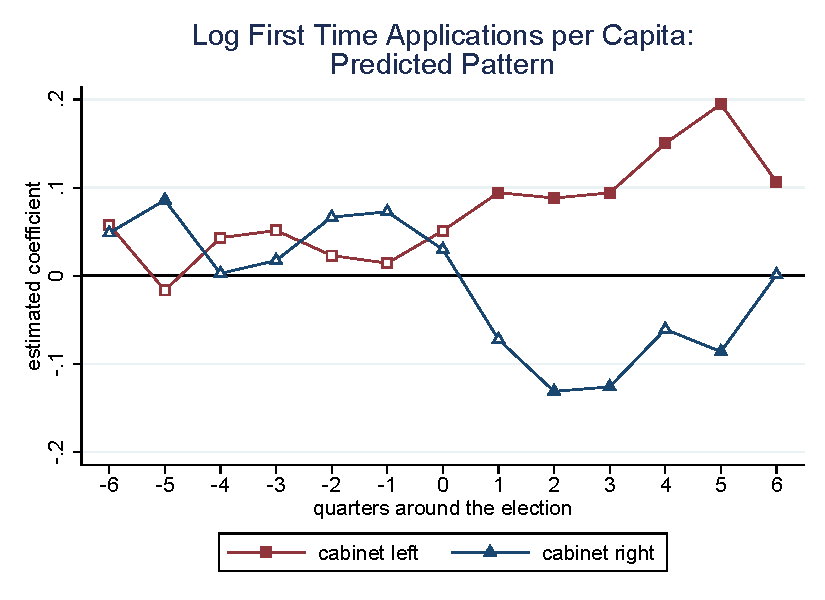
\includegraphics[width=0.7\textwidth]{figures_edited/app_graph2_R9.pdf}
	\caption{R9: log First Time Asylum Applications per Capita: Predicted Pattern}
\end{figure}

\begin{table}[!ht]\centering
	\footnotesize
	\renewcommand{\arraystretch}{1.2}
	\def\sym#1{\ifmmode^{#1}\else\(^{#1}\)\fi}
	\caption{R9: Log First Time Applications per Capita: Predicted Pattern}
	\begin{tabular}{l*{2}{c}}
		\hline\hline
		                    &\multicolumn{1}{c}{(1)}&\multicolumn{1}{c}{(2)}\\
                    &\multicolumn{1}{c}{left}&\multicolumn{1}{c}{right}\\
\hline
 6 quarters before the election&      0.0580         &      0.0486         \\
                    &    (0.0425)         &    (0.0419)         \\
 5 quarters before the election&     -0.0165         &      0.0859\sym{*}  \\
                    &    (0.0423)         &    (0.0411)         \\
 4 quarters before the election&      0.0432         &     0.00270         \\
                    &    (0.0465)         &    (0.0441)         \\
 3 quarters before the election&      0.0515         &      0.0174         \\
                    &    (0.0485)         &    (0.0466)         \\
 2 quarters before the election&      0.0230         &      0.0666         \\
                    &    (0.0437)         &    (0.0465)         \\
 1 quarters before the election&      0.0144         &      0.0727         \\
                    &    (0.0412)         &    (0.0424)         \\
Quarter of the election&      0.0512         &      0.0299         \\
                    &    (0.0388)         &    (0.0400)         \\
 1 quarters after the election&      0.0944\sym{*}  &     -0.0722         \\
                    &    (0.0384)         &    (0.0391)         \\
 2 quarters after the election&      0.0883\sym{*}  &      -0.131\sym{**} \\
                    &    (0.0378)         &    (0.0415)         \\
 3 quarters after the election&      0.0941\sym{*}  &      -0.126\sym{**} \\
                    &    (0.0394)         &    (0.0433)         \\
 4 quarters after the election&       0.150\sym{***}&     -0.0606         \\
                    &    (0.0389)         &    (0.0437)         \\
 5 quarters after the election&       0.195\sym{***}&     -0.0861\sym{*}  \\
                    &    (0.0389)         &    (0.0418)         \\
 6 quarters after the election&       0.106\sym{**} &     0.00115         \\
                    &    (0.0390)         &    (0.0377)         \\
\hline
Observations        &       23248         &       23248         \\

		\hline\hline
		\multicolumn{3}{c}{\footnotesize Standard errors in parentheses} \\
		\multicolumn{3}{c}{\footnotesize (\sym{*} \(p<0.05\), \sym{**} \(p<0.01\), \sym{***} \(p<0.001\))} \\
	\end{tabular}
\end{table}



% ===============================================================================================================


\clearpage
\FloatBarrier
\subsection{Drop country pairs with less than one first-time application per quarter on average}
\begin{table}[!ht]\centering
	\renewcommand{\arraystretch}{1.25}
	\small
	\def\sym#1{\ifmmode^{#1}\else\(^{#1}\)\fi}
	\caption{R10: Determinants of log(First time asylum applications per capita)}
	\begin{tabular}{l*{3}{c}}
		\hline\hline
		                                        &\multicolumn{1}{c}{(1)}         &\multicolumn{1}{c}{(2)}         &\multicolumn{1}{c}{(3)}         \\
\hline
Political Terror Scale                  &     0.381\sym{***}&     0.380\sym{***}&                   \\
                                        &  (0.0668)         &  (0.0665)         &                   \\
Civic Liberty (FHI)                     &     0.182         &     0.178         &                   \\
                                        &   (0.133)         &   (0.132)         &                   \\
Political Rights (FHI)                  &    0.0324         &    0.0345         &                   \\
                                        &  (0.0696)         &  (0.0697)         &                   \\
Quarterly civil war battle death (000s) &     0.190\sym{***}&     0.189\sym{***}&                   \\
                                        &  (0.0228)         &  (0.0227)         &                   \\
Log origin country real GDP per capita  &    -0.636\sym{***}&    -0.634\sym{***}&                   \\
                                        &   (0.151)         &   (0.150)         &                   \\
Log migrant stock in 2000/1             &     0.260\sym{***}&                   &     0.259\sym{***}\\
                                        &  (0.0222)         &                   &  (0.0222)         \\
Log distance from origin to destination &    -0.686\sym{*}  &                   &    -0.690\sym{*}  \\
                                        &   (0.282)         &                   &   (0.280)         \\
Log destination country real GDP per capita&    -1.291\sym{**} &    -1.254\sym{**} &    -1.231\sym{*}  \\
                                        &   (0.469)         &   (0.419)         &   (0.461)         \\
Quarterly unemployment rate at destination&   -0.0632\sym{***}&   -0.0620\sym{***}&   -0.0648\sym{***}\\
                                        &  (0.0106)         & (0.00970)         &  (0.0110)         \\
Cabinet position left * Before the election&    0.0234         &    0.0245         &    0.0145         \\
                                        &  (0.0279)         &  (0.0277)         &  (0.0277)         \\
Cabinet position left * After the election&     0.114\sym{***}&     0.110\sym{***}&     0.114\sym{***}\\
                                        &  (0.0221)         &  (0.0211)         &  (0.0223)         \\
Cabinet position right * Before the election&    0.0313         &    0.0348         &    0.0315         \\
                                        &  (0.0228)         &  (0.0215)         &  (0.0235)         \\
Cabinet position right * After the election&   -0.0757\sym{**} &   -0.0706\sym{**} &   -0.0764\sym{**} \\
                                        &  (0.0253)         &  (0.0241)         &  (0.0243)         \\
\hline
Observations                            &     24957         &     24957         &     24957         \\
Adjusted \(R^{2}\)                      &     0.472         &     0.162         &     0.479         \\
Fixed Effects                           &         O         &     D x O         &     O x T         \\
Destination dummies                     &       Yes         &        No         &       Yes         \\
Quarter-Year dummies                    &       Yes         &       Yes         &        No         \\

		\hline\hline
		\multicolumn{4}{l}{\footnotesize Standard errors in parentheses (\sym{*} \(p<0.05\), \sym{**} \(p<0.01\), \sym{***} \(p<0.001\))}\\
	\end{tabular}
\end{table}

\clearpage
\textbf{R10: Drop country pairs with less than one first-time application per quarter on average - Model 1}
\begin{figure}[!ht]
	\centering
	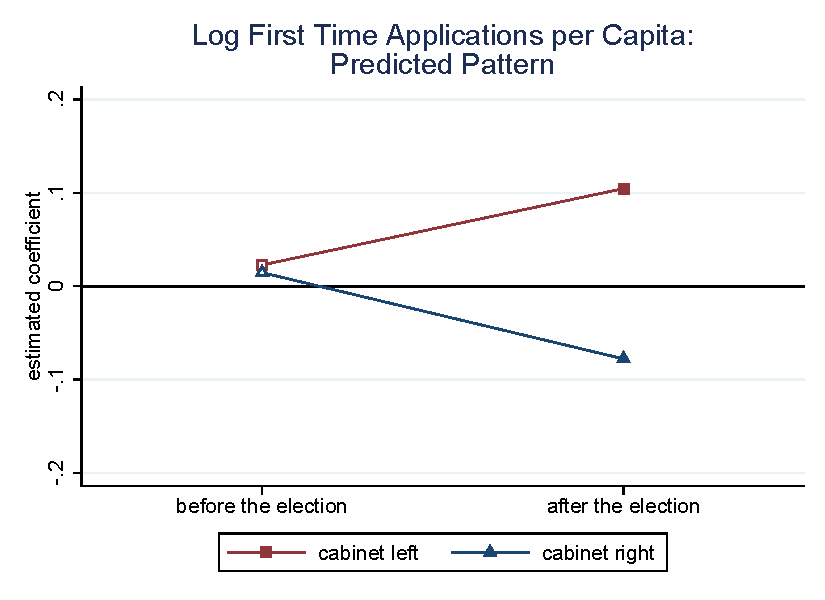
\includegraphics[width=1\textwidth]{figures_edited/app_graph1_R10.pdf}
	\caption{R10: log First Time Asylum Applications per Capita: Predicted Pattern}
\end{figure}

\begin{table}[!ht]\centering
	\renewcommand{\arraystretch}{1.25}
	\def\sym#1{\ifmmode^{#1}\else\(^{#1}\)\fi}
	\caption{R10: Log First Time Applications per Capita: Predicted Pattern}
	\begin{tabular}{l*{2}{c}}
		\hline\hline
		                    &\multicolumn{1}{c}{(1)}&\multicolumn{1}{c}{(2)}\\
                    &\multicolumn{1}{c}{left}&\multicolumn{1}{c}{right}\\
\hline
before              &      0.0245         &      0.0348         \\
                    &    (0.0277)         &    (0.0215)         \\
after               &       0.110\sym{***}&     -0.0706\sym{**} \\
                    &    (0.0211)         &    (0.0241)         \\
\hline
Observations        &       24957         &       24957         \\

		\hline\hline
		\multicolumn{3}{c}{\footnotesize Standard errors in parentheses} \\
		\multicolumn{3}{c}{\footnotesize (\sym{*} \(p<0.05\), \sym{**} \(p<0.01\), \sym{***} \(p<0.001\))}\\
	\end{tabular}
\end{table}

\clearpage
\textbf{R10: Drop country pairs with less than one first-time application per quarter on average - Model 2}
\begin{figure}[!ht]
	\centering
	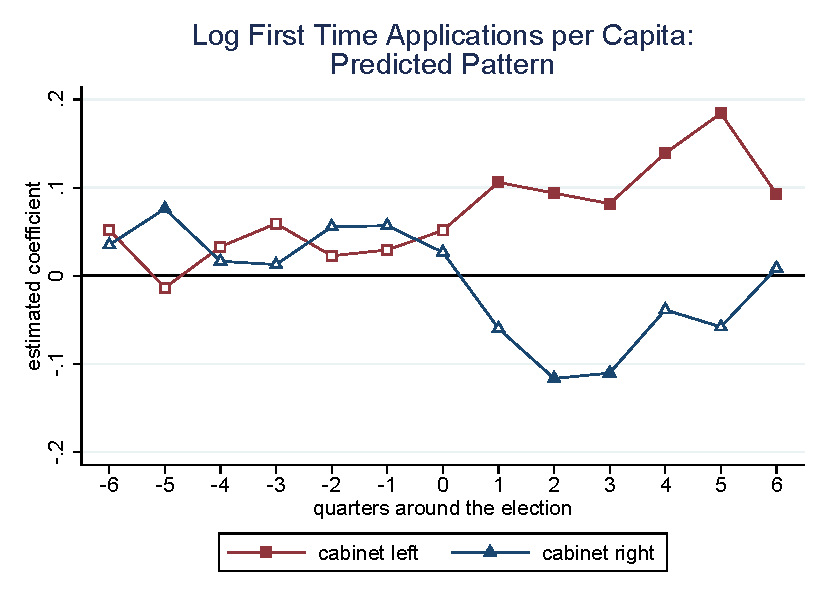
\includegraphics[width=0.7\textwidth]{figures_edited/app_graph2_R10.pdf}
	\caption{R10: log First Time Asylum Applications per Capita: Predicted Pattern}
\end{figure}

\begin{table}[!ht]\centering
	\footnotesize
	\renewcommand{\arraystretch}{1.2}
	\def\sym#1{\ifmmode^{#1}\else\(^{#1}\)\fi}
	\caption{R10: Log First Time Applications per Capita: Predicted Pattern}
	\begin{tabular}{l*{2}{c}}
		\hline\hline
		                    &\multicolumn{1}{c}{(1)}&\multicolumn{1}{c}{(2)}\\
                    &\multicolumn{1}{c}{left}&\multicolumn{1}{c}{right}\\
\hline
 6 quarters before the election&      0.0515         &      0.0348         \\
                    &    (0.0362)         &    (0.0390)         \\
 5 quarters before the election&     -0.0138         &      0.0759\sym{*}  \\
                    &    (0.0382)         &    (0.0300)         \\
 4 quarters before the election&      0.0326         &      0.0165         \\
                    &    (0.0371)         &    (0.0355)         \\
 3 quarters before the election&      0.0589         &      0.0129         \\
                    &    (0.0410)         &    (0.0292)         \\
 2 quarters before the election&      0.0226         &      0.0559         \\
                    &    (0.0326)         &    (0.0397)         \\
 1 quarters before the election&      0.0292         &      0.0570         \\
                    &    (0.0367)         &    (0.0321)         \\
Quarter of the election&      0.0515         &      0.0267         \\
                    &    (0.0354)         &    (0.0353)         \\
 1 quarters after the election&       0.106\sym{**} &     -0.0597         \\
                    &    (0.0375)         &    (0.0330)         \\
 2 quarters after the election&      0.0934\sym{**} &      -0.116\sym{***}\\
                    &    (0.0308)         &    (0.0336)         \\
 3 quarters after the election&      0.0817\sym{**} &      -0.110\sym{**} \\
                    &    (0.0302)         &    (0.0377)         \\
 4 quarters after the election&       0.139\sym{***}&     -0.0380         \\
                    &    (0.0290)         &    (0.0358)         \\
 5 quarters after the election&       0.184\sym{***}&     -0.0575         \\
                    &    (0.0290)         &    (0.0341)         \\
 6 quarters after the election&      0.0931\sym{**} &     0.00917         \\
                    &    (0.0297)         &    (0.0330)         \\
\hline
Observations        &       24957         &       24957         \\

		\hline\hline
		\multicolumn{3}{c}{\footnotesize Standard errors in parentheses} \\
		\multicolumn{3}{c}{\footnotesize (\sym{*} \(p<0.05\), \sym{**} \(p<0.01\), \sym{***} \(p<0.001\))} \\
	\end{tabular}
\end{table}



% ===============================================================================================================


\clearpage
\FloatBarrier
\subsection{Drop country pairs with less than three first-time application per quarter on average}
\begin{table}[!ht]\centering
	\renewcommand{\arraystretch}{1.25}
	\small
	\def\sym#1{\ifmmode^{#1}\else\(^{#1}\)\fi}
	\caption{R11: Determinants of log(First time asylum applications per capita)}
	\begin{tabular}{l*{3}{c}}
		\hline\hline
		                                        &\multicolumn{1}{c}{(1)}         &\multicolumn{1}{c}{(2)}         &\multicolumn{1}{c}{(3)}         \\
\hline
Political Terror Scale                  &     0.421\sym{***}&     0.423\sym{***}&                   \\
                                        &  (0.0766)         &  (0.0762)         &                   \\
Civic Liberty (FHI)                     &     0.213         &     0.211         &                   \\
                                        &   (0.143)         &   (0.141)         &                   \\
Political Rights (FHI)                  &    0.0344         &    0.0351         &                   \\
                                        &  (0.0802)         &  (0.0803)         &                   \\
Quarterly civil war battle death (000s) &     0.201\sym{***}&     0.199\sym{***}&                   \\
                                        &  (0.0253)         &  (0.0251)         &                   \\
Log origin country real GDP per capita  &    -0.642\sym{***}&    -0.635\sym{***}&                   \\
                                        &   (0.162)         &   (0.161)         &                   \\
Log migrant stock in 2000/1             &     0.264\sym{***}&                   &     0.263\sym{***}\\
                                        &  (0.0221)         &                   &  (0.0220)         \\
Log distance from origin to destination &    -0.555         &                   &    -0.563         \\
                                        &   (0.299)         &                   &   (0.297)         \\
Log destination country real GDP per capita&    -1.193\sym{*}  &    -1.402\sym{*}  &    -0.833         \\
                                        &   (0.583)         &   (0.531)         &   (0.527)         \\
Quarterly unemployment rate at destination&   -0.0708\sym{***}&   -0.0731\sym{***}&   -0.0678\sym{***}\\
                                        &  (0.0124)         &  (0.0117)         &  (0.0125)         \\
Cabinet position left * Before the election&   0.00134         &   0.00124         &  -0.00872         \\
                                        &  (0.0299)         &  (0.0301)         &  (0.0322)         \\
Cabinet position left * After the election&     0.115\sym{***}&     0.107\sym{***}&     0.107\sym{***}\\
                                        &  (0.0234)         &  (0.0217)         &  (0.0245)         \\
Cabinet position right * Before the election&    0.0465         &    0.0480         &    0.0496         \\
                                        &  (0.0270)         &  (0.0260)         &  (0.0271)         \\
Cabinet position right * After the election&   -0.0997\sym{***}&   -0.0953\sym{***}&   -0.0950\sym{***}\\
                                        &  (0.0262)         &  (0.0251)         &  (0.0254)         \\
\hline
Observations                            &     21989         &     21989         &     21989         \\
Adjusted \(R^{2}\)                      &     0.427         &     0.186         &     0.427         \\
Fixed Effects                           &         O         &     D x O         &     O x T         \\
Destination dummies                     &       Yes         &        No         &       Yes         \\
Quarter-Year dummies                    &       Yes         &       Yes         &        No         \\

		\hline\hline
		\multicolumn{4}{l}{\footnotesize Standard errors in parentheses (\sym{*} \(p<0.05\), \sym{**} \(p<0.01\), \sym{***} \(p<0.001\))}\\
	\end{tabular}
\end{table}

\clearpage
\textbf{R11: Drop country pairs with less than three first-time application per quarter on average - Model 1}
\begin{figure}[!ht]
	\centering
	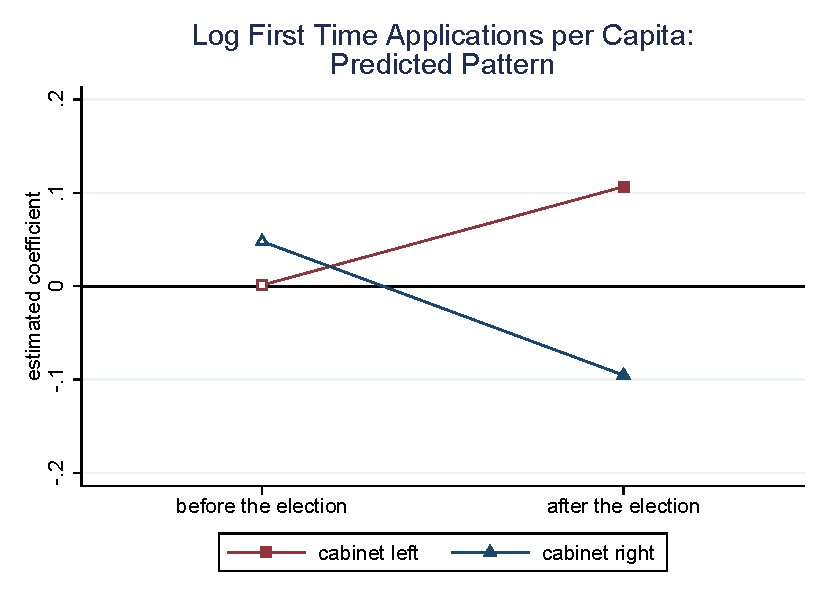
\includegraphics[width=1\textwidth]{figures_edited/app_graph1_R11.pdf}
	\caption{R11: log First Time Asylum Applications per Capita: Predicted Pattern}
\end{figure}

\begin{table}[!ht]\centering
	\renewcommand{\arraystretch}{1.25}
	\def\sym#1{\ifmmode^{#1}\else\(^{#1}\)\fi}
	\caption{R11: Log First Time Applications per Capita: Predicted Pattern}
	\begin{tabular}{l*{2}{c}}
		\hline\hline
		                    &\multicolumn{1}{c}{(1)}&\multicolumn{1}{c}{(2)}\\
                    &\multicolumn{1}{c}{left}&\multicolumn{1}{c}{right}\\
\hline
before              &     0.00144         &      0.0473         \\
                    &    (0.0300)         &    (0.0260)         \\
after               &       0.106\sym{***}&     -0.0949\sym{***}\\
                    &    (0.0217)         &    (0.0251)         \\
\hline
Observations        &       21989         &       21989         \\

		\hline\hline
		\multicolumn{3}{c}{\footnotesize Standard errors in parentheses} \\
		\multicolumn{3}{c}{\footnotesize (\sym{*} \(p<0.05\), \sym{**} \(p<0.01\), \sym{***} \(p<0.001\))}\\
	\end{tabular}
\end{table}

\clearpage
\textbf{R11: Drop country pairs with less than three first-time application per quarter on average - Model 2}
\begin{figure}[!ht]
	\centering
	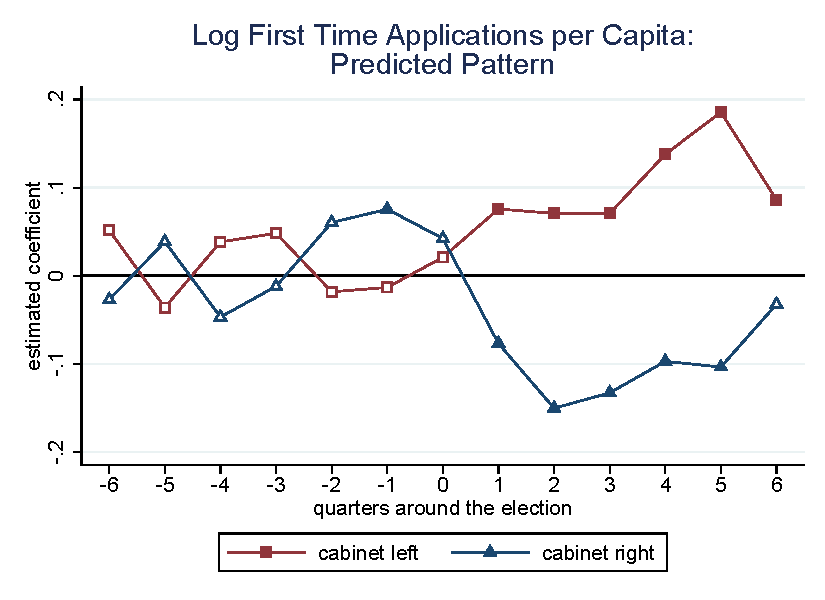
\includegraphics[width=0.7\textwidth]{figures_edited/app_graph2_R11.pdf}
	\caption{R11: log First Time Asylum Applications per Capita: Predicted Pattern}
\end{figure}

\begin{table}[!ht]\centering
	\footnotesize
	\renewcommand{\arraystretch}{1.2}
	\def\sym#1{\ifmmode^{#1}\else\(^{#1}\)\fi}
	\caption{R11: Log First Time Applications per Capita: Predicted Pattern}
	\begin{tabular}{l*{2}{c}}
		\hline\hline
		                    &\multicolumn{1}{c}{(1)}&\multicolumn{1}{c}{(2)}\\
                    &\multicolumn{1}{c}{left}&\multicolumn{1}{c}{right}\\
\hline
 6 quarters before the election&      0.0407         &      0.0492         \\
                    &    (0.0403)         &    (0.0426)         \\
 5 quarters before the election&     -0.0351         &      0.0899\sym{**} \\
                    &    (0.0401)         &    (0.0324)         \\
 4 quarters before the election&      0.0344         &      0.0104         \\
                    &    (0.0403)         &    (0.0411)         \\
 3 quarters before the election&      0.0486         &     0.00502         \\
                    &    (0.0454)         &    (0.0306)         \\
 2 quarters before the election&     -0.0125         &      0.0737         \\
                    &    (0.0340)         &    (0.0403)         \\
 1 quarters before the election&     -0.0129         &      0.0849\sym{*}  \\
                    &    (0.0373)         &    (0.0379)         \\
Quarter of the election&      0.0300         &      0.0496         \\
                    &    (0.0384)         &    (0.0454)         \\
 1 quarters after the election&      0.0827\sym{*}  &     -0.0727\sym{*}  \\
                    &    (0.0404)         &    (0.0347)         \\
 2 quarters after the election&      0.0796\sym{*}  &      -0.138\sym{***}\\
                    &    (0.0317)         &    (0.0358)         \\
 3 quarters after the election&      0.0776\sym{*}  &      -0.124\sym{**} \\
                    &    (0.0320)         &    (0.0432)         \\
 4 quarters after the election&       0.148\sym{***}&     -0.0765\sym{*}  \\
                    &    (0.0286)         &    (0.0339)         \\
 5 quarters after the election&       0.198\sym{***}&     -0.0915\sym{*}  \\
                    &    (0.0278)         &    (0.0381)         \\
 6 quarters after the election&      0.0936\sym{**} &     -0.0167         \\
                    &    (0.0305)         &    (0.0323)         \\
\hline
Observations        &       21989         &       21989         \\

		\hline\hline
		\multicolumn{3}{c}{\footnotesize Standard errors in parentheses} \\
		\multicolumn{3}{c}{\footnotesize (\sym{*} \(p<0.05\), \sym{**} \(p<0.01\), \sym{***} \(p<0.001\))} \\
	\end{tabular}
\end{table}



% ===============================================================================================================


\clearpage
\FloatBarrier
\subsection{Use normalized cabinet position to determine cabinet left-right dummies}
\begin{table}[!ht]\centering
	\renewcommand{\arraystretch}{1.25}
	\small
	\def\sym#1{\ifmmode^{#1}\else\(^{#1}\)\fi}
	\caption{R12: Determinants of log(First time asylum applications per capita)}
	\begin{tabular}{l*{3}{c}}
		\hline\hline
		                                        &\multicolumn{1}{c}{(1)}         &\multicolumn{1}{c}{(2)}         &\multicolumn{1}{c}{(3)}         \\
\hline
Political Terror Scale                  &     0.407\sym{***}&     0.407\sym{***}&                   \\
                                        &  (0.0713)         &  (0.0708)         &                   \\
Civic Liberty (FHI)                     &     0.190         &     0.189         &                   \\
                                        &   (0.139)         &   (0.138)         &                   \\
Political Rights (FHI)                  &    0.0402         &    0.0423         &                   \\
                                        &  (0.0757)         &  (0.0757)         &                   \\
Quarterly civil war battle death (000s) &     0.188\sym{***}&     0.186\sym{***}&                   \\
                                        &  (0.0237)         &  (0.0235)         &                   \\
Log origin country real GDP per capita  &    -0.656\sym{***}&    -0.657\sym{***}&                   \\
                                        &   (0.165)         &   (0.163)         &                   \\
Log migrant stock in 2000/1             &     0.263\sym{***}&                   &     0.263\sym{***}\\
                                        &  (0.0215)         &                   &  (0.0214)         \\
Log distance from origin to destination &    -0.547         &                   &    -0.552         \\
                                        &   (0.296)         &                   &   (0.295)         \\
Log destination country real GDP per capita&    -1.409\sym{**} &    -1.486\sym{**} &    -1.146\sym{*}  \\
                                        &   (0.501)         &   (0.450)         &   (0.477)         \\
Quarterly unemployment rate at destination&   -0.0709\sym{***}&   -0.0721\sym{***}&   -0.0691\sym{***}\\
                                        &  (0.0116)         &  (0.0110)         &  (0.0118)         \\
Cabinet position left * Before the election&    0.0104         &   0.00976         &  -0.00337         \\
                                        &  (0.0290)         &  (0.0291)         &  (0.0306)         \\
Cabinet position left * After the election&     0.114\sym{***}&     0.106\sym{***}&     0.107\sym{***}\\
                                        &  (0.0243)         &  (0.0230)         &  (0.0251)         \\
Cabinet position right * Before the election&    0.0495\sym{*}  &    0.0513\sym{*}  &    0.0519\sym{*}  \\
                                        &  (0.0240)         &  (0.0231)         &  (0.0238)         \\
Cabinet position right * After the election&   -0.0830\sym{***}&   -0.0777\sym{***}&   -0.0836\sym{***}\\
                                        &  (0.0225)         &  (0.0217)         &  (0.0223)         \\
\hline
Observations                            &     23248         &     23248         &     23248         \\
Adjusted \(R^{2}\)                      &     0.447         &     0.176         &     0.451         \\
Fixed Effects                           &         O         &     D x O         &     O x T         \\
Destination dummies                     &       Yes         &        No         &       Yes         \\
Quarter-Year dummies                    &       Yes         &       Yes         &        No         \\

		\hline\hline
		\multicolumn{4}{l}{\footnotesize Standard errors in parentheses (\sym{*} \(p<0.05\), \sym{**} \(p<0.01\), \sym{***} \(p<0.001\))}\\
	\end{tabular}
\end{table}

\clearpage
\textbf{R12: Use normalized cabinet position to determine cabinet left-right dummies - Model 1}
\begin{figure}[!ht]
	\centering
	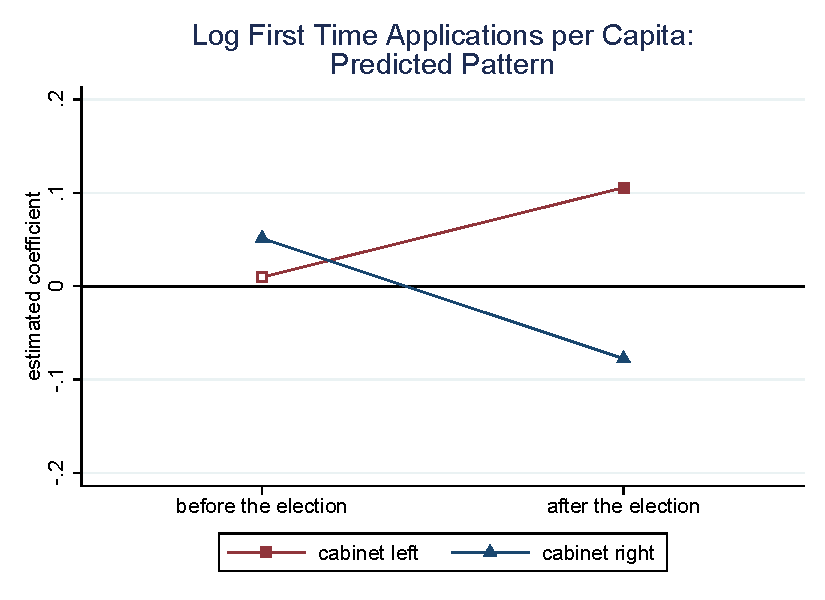
\includegraphics[width=1\textwidth]{figures_edited/app_graph1_R12.pdf}
	\caption{R12: log First Time Asylum Applications per Capita: Predicted Pattern}
\end{figure}

\begin{table}[!ht]\centering
	\renewcommand{\arraystretch}{1.25}
	\def\sym#1{\ifmmode^{#1}\else\(^{#1}\)\fi}
	\caption{R12: Log First Time Applications per Capita: Predicted Pattern}
	\begin{tabular}{l*{2}{c}}
		\hline\hline
		                    &\multicolumn{1}{c}{(1)}&\multicolumn{1}{c}{(2)}\\
                    &\multicolumn{1}{c}{left}&\multicolumn{1}{c}{right}\\
\hline
before              &     0.00976         &      0.0513\sym{*}  \\
                    &    (0.0291)         &    (0.0231)         \\
after               &       0.106\sym{***}&     -0.0777\sym{***}\\
                    &    (0.0230)         &    (0.0217)         \\
\hline
Observations        &       23248         &       23248         \\

		\hline\hline
		\multicolumn{3}{c}{\footnotesize Standard errors in parentheses} \\
		\multicolumn{3}{c}{\footnotesize (\sym{*} \(p<0.05\), \sym{**} \(p<0.01\), \sym{***} \(p<0.001\))}\\
	\end{tabular}
\end{table}

\clearpage
\textbf{R12: Use normalized cabinet position to determine cabinet left-right dummies - Model 2}
\begin{figure}[!ht]
	\centering
	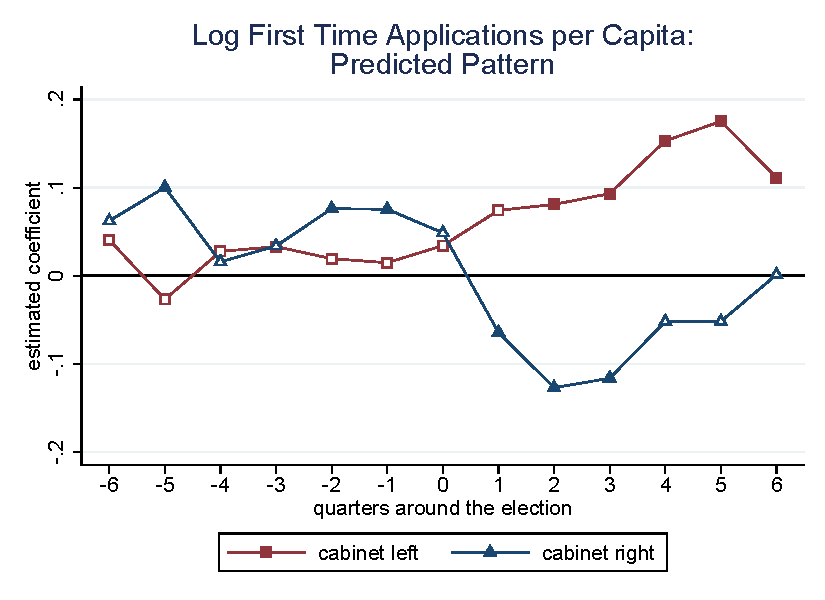
\includegraphics[width=0.7\textwidth]{figures_edited/app_graph2_R12.pdf}
	\caption{R12: log First Time Asylum Applications per Capita: Predicted Pattern}
\end{figure}

\begin{table}[!ht]\centering
	\footnotesize
	\renewcommand{\arraystretch}{1.2}
	\def\sym#1{\ifmmode^{#1}\else\(^{#1}\)\fi}
	\caption{R12: Log First Time Applications per Capita: Predicted Pattern}
	\begin{tabular}{l*{2}{c}}
		\hline\hline
		                    &\multicolumn{1}{c}{(1)}&\multicolumn{1}{c}{(2)}\\
                    &\multicolumn{1}{c}{left}&\multicolumn{1}{c}{right}\\
\hline
 6 quarters before the election&      0.0409         &      0.0623         \\
                    &    (0.0379)         &    (0.0421)         \\
 5 quarters before the election&     -0.0268         &       0.100\sym{**} \\
                    &    (0.0385)         &    (0.0321)         \\
 4 quarters before the election&      0.0277         &      0.0158         \\
                    &    (0.0390)         &    (0.0371)         \\
 3 quarters before the election&      0.0332         &      0.0338         \\
                    &    (0.0411)         &    (0.0308)         \\
 2 quarters before the election&      0.0195         &      0.0761\sym{*}  \\
                    &    (0.0344)         &    (0.0386)         \\
 1 quarters before the election&      0.0149         &      0.0755\sym{*}  \\
                    &    (0.0378)         &    (0.0357)         \\
Quarter of the election&      0.0343         &      0.0487         \\
                    &    (0.0382)         &    (0.0377)         \\
 1 quarters after the election&      0.0742         &     -0.0643\sym{*}  \\
                    &    (0.0392)         &    (0.0298)         \\
 2 quarters after the election&      0.0810\sym{*}  &      -0.127\sym{***}\\
                    &    (0.0318)         &    (0.0364)         \\
 3 quarters after the election&      0.0933\sym{**} &      -0.116\sym{**} \\
                    &    (0.0338)         &    (0.0356)         \\
 4 quarters after the election&       0.153\sym{***}&     -0.0519         \\
                    &    (0.0301)         &    (0.0333)         \\
 5 quarters after the election&       0.175\sym{***}&     -0.0517         \\
                    &    (0.0277)         &    (0.0328)         \\
 6 quarters after the election&       0.112\sym{***}&     0.00126         \\
                    &    (0.0324)         &    (0.0306)         \\
\hline
Observations        &       23248         &       23248         \\

		\hline\hline
		\multicolumn{3}{c}{\footnotesize Standard errors in parentheses} \\
		\multicolumn{3}{c}{\footnotesize (\sym{*} \(p<0.05\), \sym{**} \(p<0.01\), \sym{***} \(p<0.001\))} \\
	\end{tabular}
\end{table}



% ===============================================================================================================


\clearpage
\FloatBarrier
\subsection{Split cabinet position at 5 to determine cabinet left-right dummies}
\begin{table}[!ht]\centering
	\renewcommand{\arraystretch}{1.25}
	\small
	\def\sym#1{\ifmmode^{#1}\else\(^{#1}\)\fi}
	\caption{R13: Determinants of log(First time asylum applications per capita)}
	\begin{tabular}{l*{3}{c}}
		\hline\hline
		                                        &\multicolumn{1}{c}{(1)}         &\multicolumn{1}{c}{(2)}         &\multicolumn{1}{c}{(3)}         \\
\hline
Political Terror Scale                  &     0.407\sym{***}&     0.407\sym{***}&                   \\
                                        &  (0.0713)         &  (0.0707)         &                   \\
Civic Liberty (FHI)                     &     0.190         &     0.189         &                   \\
                                        &   (0.140)         &   (0.138)         &                   \\
Political Rights (FHI)                  &    0.0397         &    0.0418         &                   \\
                                        &  (0.0758)         &  (0.0758)         &                   \\
Quarterly civil war battle death (000s) &     0.187\sym{***}&     0.185\sym{***}&                   \\
                                        &  (0.0237)         &  (0.0236)         &                   \\
Log origin country real GDP per capita  &    -0.657\sym{***}&    -0.659\sym{***}&                   \\
                                        &   (0.165)         &   (0.163)         &                   \\
Log migrant stock in 2000/1             &     0.263\sym{***}&                   &     0.263\sym{***}\\
                                        &  (0.0215)         &                   &  (0.0214)         \\
Log distance from origin to destination &    -0.547         &                   &    -0.553         \\
                                        &   (0.296)         &                   &   (0.295)         \\
Log destination country real GDP per capita&    -1.472\sym{**} &    -1.546\sym{**} &    -1.224\sym{*}  \\
                                        &   (0.492)         &   (0.445)         &   (0.467)         \\
Quarterly unemployment rate at destination&   -0.0718\sym{***}&   -0.0731\sym{***}&   -0.0701\sym{***}\\
                                        &  (0.0115)         &  (0.0109)         &  (0.0118)         \\
Cabinet position left * Before the election&   0.00818         &   0.00882         &   -0.0100         \\
                                        &  (0.0321)         &  (0.0319)         &  (0.0334)         \\
Cabinet position left * After the election&     0.120\sym{***}&     0.110\sym{***}&     0.109\sym{***}\\
                                        &  (0.0264)         &  (0.0245)         &  (0.0270)         \\
Cabinet position right * Before the election&    0.0507\sym{*}  &    0.0505\sym{*}  &    0.0548\sym{*}  \\
                                        &  (0.0214)         &  (0.0202)         &  (0.0214)         \\
Cabinet position right * After the election&   -0.0422         &   -0.0388         &   -0.0408         \\
                                        &  (0.0226)         &  (0.0218)         &  (0.0227)         \\
\hline
Observations                            &     23248         &     23248         &     23248         \\
Adjusted \(R^{2}\)                      &     0.446         &     0.175         &     0.450         \\
Fixed Effects                           &         O         &     D x O         &     O x T         \\
Destination dummies                     &       Yes         &        No         &       Yes         \\
Quarter-Year dummies                    &       Yes         &       Yes         &        No         \\

		\hline\hline
		\multicolumn{4}{l}{\footnotesize Standard errors in parentheses (\sym{*} \(p<0.05\), \sym{**} \(p<0.01\), \sym{***} \(p<0.001\))}\\
	\end{tabular}
\end{table}

\clearpage
\textbf{R13: Split cabinet position at 5 to determine cabinet left-right dummies - Model 1}
\begin{figure}[!ht]
	\centering
	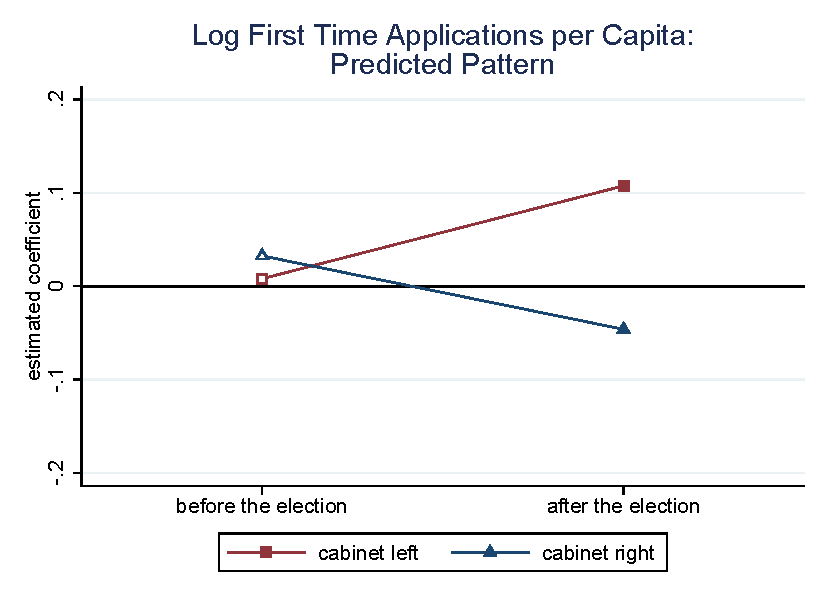
\includegraphics[width=1\textwidth]{figures_edited/app_graph1_R13.pdf}
	\caption{R13: log First Time Asylum Applications per Capita: Predicted Pattern}
\end{figure}

\begin{table}[!ht]\centering
	\renewcommand{\arraystretch}{1.25}
	\def\sym#1{\ifmmode^{#1}\else\(^{#1}\)\fi}
	\caption{R13: Log First Time Applications per Capita: Predicted Pattern}
	\begin{tabular}{l*{2}{c}}
		\hline\hline
		                    &\multicolumn{1}{c}{(1)}&\multicolumn{1}{c}{(2)}\\
                    &\multicolumn{1}{c}{left}&\multicolumn{1}{c}{right}\\
\hline
before              &     0.00882         &      0.0505\sym{*}  \\
                    &    (0.0319)         &    (0.0202)         \\
after               &       0.110\sym{***}&     -0.0388         \\
                    &    (0.0245)         &    (0.0218)         \\
\hline
Observations        &       23248         &       23248         \\

		\hline\hline
		\multicolumn{3}{c}{\footnotesize Standard errors in parentheses} \\
		\multicolumn{3}{c}{\footnotesize (\sym{*} \(p<0.05\), \sym{**} \(p<0.01\), \sym{***} \(p<0.001\))}\\
	\end{tabular}
\end{table}

\clearpage
\textbf{R13: Split cabinet position at 5 to determine cabinet left-right dummies - Model 2}
\begin{figure}[!ht]
	\centering
	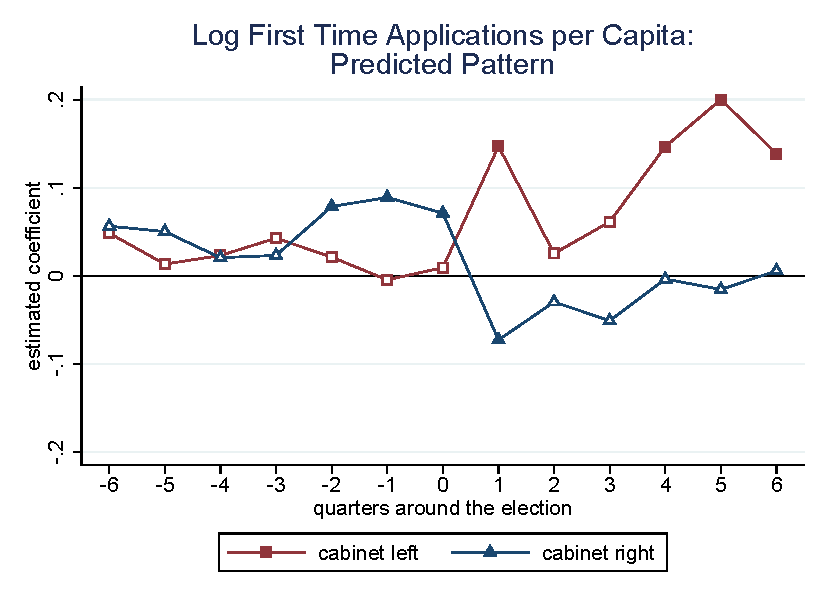
\includegraphics[width=0.7\textwidth]{figures_edited/app_graph2_R13.pdf}
	\caption{R13: log First Time Asylum Applications per Capita: Predicted Pattern}
\end{figure}

\begin{table}[!ht]\centering
	\footnotesize
	\renewcommand{\arraystretch}{1.2}
	\def\sym#1{\ifmmode^{#1}\else\(^{#1}\)\fi}
	\caption{R13: Log First Time Applications per Capita: Predicted Pattern}
	\begin{tabular}{l*{2}{c}}
		\hline\hline
		                    &\multicolumn{1}{c}{(1)}&\multicolumn{1}{c}{(2)}\\
                    &\multicolumn{1}{c}{left}&\multicolumn{1}{c}{right}\\
\hline
 6 quarters before the election&      0.0486         &      0.0566         \\
                    &    (0.0409)         &    (0.0320)         \\
 5 quarters before the election&      0.0135         &      0.0504         \\
                    &    (0.0412)         &    (0.0271)         \\
 4 quarters before the election&      0.0233         &      0.0208         \\
                    &    (0.0408)         &    (0.0350)         \\
 3 quarters before the election&      0.0430         &      0.0234         \\
                    &    (0.0458)         &    (0.0281)         \\
 2 quarters before the election&      0.0214         &      0.0788\sym{*}  \\
                    &    (0.0362)         &    (0.0381)         \\
 1 quarters before the election&    -0.00435         &      0.0892\sym{*}  \\
                    &    (0.0392)         &    (0.0361)         \\
Quarter of the election&     0.00948         &      0.0713\sym{*}  \\
                    &    (0.0441)         &    (0.0359)         \\
 1 quarters after the election&       0.147\sym{***}&     -0.0726\sym{*}  \\
                    &    (0.0412)         &    (0.0323)         \\
 2 quarters after the election&      0.0256         &     -0.0295         \\
                    &    (0.0344)         &    (0.0314)         \\
 3 quarters after the election&      0.0614         &     -0.0507         \\
                    &    (0.0375)         &    (0.0345)         \\
 4 quarters after the election&       0.147\sym{***}&    -0.00350         \\
                    &    (0.0373)         &    (0.0308)         \\
 5 quarters after the election&       0.200\sym{***}&     -0.0153         \\
                    &    (0.0345)         &    (0.0318)         \\
 6 quarters after the election&       0.139\sym{***}&     0.00590         \\
                    &    (0.0315)         &    (0.0292)         \\
\hline
Observations        &       23248         &       23248         \\

		\hline\hline
		\multicolumn{3}{c}{\footnotesize Standard errors in parentheses} \\
		\multicolumn{3}{c}{\footnotesize (\sym{*} \(p<0.05\), \sym{**} \(p<0.01\), \sym{***} \(p<0.001\))} \\
	\end{tabular}
\end{table}



% ===============================================================================================================


\clearpage
\FloatBarrier
\subsection{Use only 5 quarters around the election}
\begin{table}[!ht]\centering
	\renewcommand{\arraystretch}{1.25}
	\small
	\def\sym#1{\ifmmode^{#1}\else\(^{#1}\)\fi}
	\caption{R14: Determinants of log(First time asylum applications per capita)}
	\begin{tabular}{l*{3}{c}}
		\hline\hline
		                                        &\multicolumn{1}{c}{(1)}         &\multicolumn{1}{c}{(2)}         &\multicolumn{1}{c}{(3)}         \\
\hline
Political Terror Scale                  &     0.416\sym{***}&     0.416\sym{***}&                   \\
                                        &  (0.0712)         &  (0.0707)         &                   \\
Civic Liberty (FHI)                     &     0.191         &     0.190         &                   \\
                                        &   (0.138)         &   (0.136)         &                   \\
Political Rights (FHI)                  &    0.0369         &    0.0391         &                   \\
                                        &  (0.0756)         &  (0.0758)         &                   \\
Quarterly civil war battle death (000s) &     0.126\sym{***}&     0.125\sym{***}&                   \\
                                        &  (0.0141)         &  (0.0139)         &                   \\
Log origin country real GDP per capita  &    -0.649\sym{***}&    -0.651\sym{***}&                   \\
                                        &   (0.169)         &   (0.167)         &                   \\
Log migrant stock in 2000/1             &     0.264\sym{***}&                   &     0.263\sym{***}\\
                                        &  (0.0215)         &                   &  (0.0214)         \\
Log distance from origin to destination &    -0.547         &                   &    -0.552         \\
                                        &   (0.296)         &                   &   (0.295)         \\
Log destination country real GDP per capita&    -1.465\sym{**} &    -1.538\sym{**} &    -1.205\sym{*}  \\
                                        &   (0.501)         &   (0.449)         &   (0.476)         \\
Quarterly unemployment rate at destination&   -0.0730\sym{***}&   -0.0741\sym{***}&   -0.0711\sym{***}\\
                                        &  (0.0117)         &  (0.0110)         &  (0.0119)         \\
Cabinet position left * Before the election&    0.0186         &    0.0173         &   0.00469         \\
                                        &  (0.0302)         &  (0.0303)         &  (0.0312)         \\
Cabinet position left * After the election&     0.112\sym{***}&     0.104\sym{***}&     0.107\sym{***}\\
                                        &  (0.0241)         &  (0.0227)         &  (0.0243)         \\
Cabinet position right * Before the election&    0.0162         &    0.0186         &    0.0166         \\
                                        &  (0.0245)         &  (0.0236)         &  (0.0241)         \\
Cabinet position right * After the election&    -0.121\sym{***}&    -0.115\sym{***}&    -0.123\sym{***}\\
                                        &  (0.0246)         &  (0.0241)         &  (0.0240)         \\
\hline
Observations                            &     23248         &     23248         &     23248         \\
Adjusted \(R^{2}\)                      &     0.447         &     0.177         &     0.451         \\
Fixed Effects                           &         O         &     D x O         &     O x T         \\
Destination dummies                     &       Yes         &        No         &       Yes         \\
Quarter-Year dummies                    &       Yes         &       Yes         &        No         \\

		\hline\hline
		\multicolumn{4}{l}{\footnotesize Standard errors in parentheses (\sym{*} \(p<0.05\), \sym{**} \(p<0.01\), \sym{***} \(p<0.001\))}\\
	\end{tabular}
\end{table}

\clearpage
\textbf{R14: Use only 5 quarters around the election - Model 1}
\begin{figure}[!ht]
	\centering
	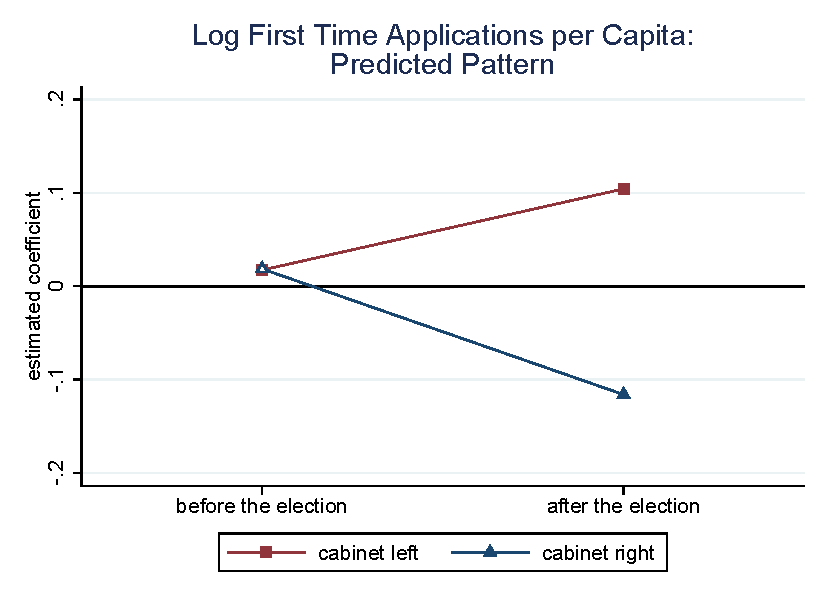
\includegraphics[width=1\textwidth]{figures_edited/app_graph1_R14.pdf}
	\caption{R14: log First Time Asylum Applications per Capita: Predicted Pattern}
\end{figure}

\begin{table}[!ht]\centering
	\renewcommand{\arraystretch}{1.25}
	\def\sym#1{\ifmmode^{#1}\else\(^{#1}\)\fi}
	\caption{R14: Log First Time Applications per Capita: Predicted Pattern}
	\begin{tabular}{l*{2}{c}}
		\hline\hline
		                    &\multicolumn{1}{c}{(1)}&\multicolumn{1}{c}{(2)}\\
                    &\multicolumn{1}{c}{left}&\multicolumn{1}{c}{right}\\
\hline
before              &      0.0173         &      0.0186         \\
                    &    (0.0303)         &    (0.0236)         \\
after               &       0.104\sym{***}&      -0.115\sym{***}\\
                    &    (0.0227)         &    (0.0241)         \\
\hline
Observations        &       23248         &       23248         \\

		\hline\hline
		\multicolumn{3}{c}{\footnotesize Standard errors in parentheses} \\
		\multicolumn{3}{c}{\footnotesize (\sym{*} \(p<0.05\), \sym{**} \(p<0.01\), \sym{***} \(p<0.001\))}\\
	\end{tabular}
\end{table}

\clearpage
\textbf{R14: Use only 5 quarters around the election - Model 2}
\begin{figure}[!ht]
	\centering
	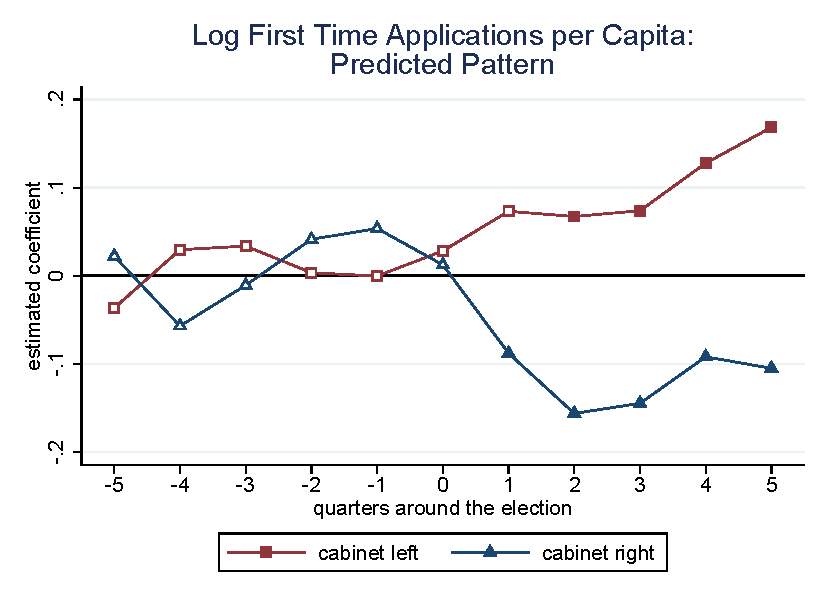
\includegraphics[width=0.7\textwidth]{figures_edited/app_graph2_R14.pdf}
	\caption{R14: log First Time Asylum Applications per Capita: Predicted Pattern}
\end{figure}

\begin{table}[!ht]\centering
	\footnotesize
	\renewcommand{\arraystretch}{1.2}
	\def\sym#1{\ifmmode^{#1}\else\(^{#1}\)\fi}
	\caption{R14: Log First Time Applications per Capita: Predicted Pattern}
	\begin{tabular}{l*{2}{c}}
		\hline\hline
		                    &\multicolumn{1}{c}{(1)}&\multicolumn{1}{c}{(2)}\\
                    &\multicolumn{1}{c}{left}&\multicolumn{1}{c}{right}\\
\hline
 5 quarters before the election&     -0.0383         &      0.0705\sym{*}  \\
                    &    (0.0373)         &    (0.0317)         \\
 4 quarters before the election&      0.0269         &     -0.0115         \\
                    &    (0.0393)         &    (0.0373)         \\
 3 quarters before the election&      0.0301         &    0.000633         \\
                    &    (0.0412)         &    (0.0300)         \\
 2 quarters before the election&     0.00308         &      0.0492         \\
                    &    (0.0332)         &    (0.0384)         \\
 1 quarters before the election&    -0.00248         &      0.0562         \\
                    &    (0.0373)         &    (0.0345)         \\
Quarter of the election&      0.0330         &      0.0139         \\
                    &    (0.0375)         &    (0.0385)         \\
 1 quarters after the election&      0.0743         &     -0.0912\sym{**} \\
                    &    (0.0392)         &    (0.0323)         \\
 2 quarters after the election&      0.0694\sym{*}  &      -0.150\sym{***}\\
                    &    (0.0309)         &    (0.0357)         \\
 3 quarters after the election&      0.0757\sym{*}  &      -0.143\sym{***}\\
                    &    (0.0325)         &    (0.0383)         \\
 4 quarters after the election&       0.134\sym{***}&     -0.0781\sym{*}  \\
                    &    (0.0279)         &    (0.0342)         \\
 5 quarters after the election&       0.176\sym{***}&      -0.100\sym{**} \\
                    &    (0.0272)         &    (0.0358)         \\
\hline
Observations        &       23248         &       23248         \\

		\hline\hline
		\multicolumn{3}{c}{\footnotesize Standard errors in parentheses} \\
		\multicolumn{3}{c}{\footnotesize (\sym{*} \(p<0.05\), \sym{**} \(p<0.01\), \sym{***} \(p<0.001\))} \\
	\end{tabular}
\end{table}



% ===============================================================================================================


\clearpage
\FloatBarrier
\subsection{Use only 4 quarters around the election}
\begin{table}[!ht]\centering
	\renewcommand{\arraystretch}{1.25}
	\small
	\def\sym#1{\ifmmode^{#1}\else\(^{#1}\)\fi}
	\caption{R15: Determinants of log(First time asylum applications per capita)}
	\begin{tabular}{l*{3}{c}}
		\hline\hline
		                                        &\multicolumn{1}{c}{(1)}         &\multicolumn{1}{c}{(2)}         &\multicolumn{1}{c}{(3)}         \\
\hline
Political Terror Scale                  &     0.407\sym{***}&     0.407\sym{***}&                   \\
                                        &  (0.0713)         &  (0.0707)         &                   \\
Civic Liberty (FHI)                     &     0.190         &     0.189         &                   \\
                                        &   (0.140)         &   (0.138)         &                   \\
Political Rights (FHI)                  &    0.0403         &    0.0424         &                   \\
                                        &  (0.0758)         &  (0.0758)         &                   \\
Quarterly civil war battle death (000s) &     0.187\sym{***}&     0.186\sym{***}&                   \\
                                        &  (0.0237)         &  (0.0236)         &                   \\
Log origin country real GDP per capita  &    -0.656\sym{***}&    -0.658\sym{***}&                   \\
                                        &   (0.165)         &   (0.163)         &                   \\
Log migrant stock in 2000/1             &     0.263\sym{***}&                   &     0.263\sym{***}\\
                                        &  (0.0215)         &                   &  (0.0214)         \\
Log distance from origin to destination &    -0.547         &                   &    -0.552         \\
                                        &   (0.296)         &                   &   (0.295)         \\
Log destination country real GDP per capita&    -1.512\sym{**} &    -1.582\sym{**} &    -1.240\sym{*}  \\
                                        &   (0.505)         &   (0.452)         &   (0.479)         \\
Quarterly unemployment rate at destination&   -0.0728\sym{***}&   -0.0740\sym{***}&   -0.0710\sym{***}\\
                                        &  (0.0116)         &  (0.0110)         &  (0.0119)         \\
Cabinet position left * Before the election&   0.00511         &   0.00399         &  -0.00916         \\
                                        &  (0.0285)         &  (0.0283)         &  (0.0294)         \\
Cabinet position left * After the election&    0.0879\sym{***}&    0.0801\sym{**} &    0.0849\sym{***}\\
                                        &  (0.0240)         &  (0.0229)         &  (0.0241)         \\
Cabinet position right * Before the election&    0.0195         &    0.0211         &    0.0196         \\
                                        &  (0.0238)         &  (0.0228)         &  (0.0233)         \\
Cabinet position right * After the election&    -0.132\sym{***}&    -0.126\sym{***}&    -0.132\sym{***}\\
                                        &  (0.0247)         &  (0.0237)         &  (0.0245)         \\
\hline
Observations                            &     23248         &     23248         &     23248         \\
Adjusted \(R^{2}\)                      &     0.446         &     0.175         &     0.450         \\
Fixed Effects                           &         O         &     D x O         &     O x T         \\
Destination dummies                     &       Yes         &        No         &       Yes         \\
Quarter-Year dummies                    &       Yes         &       Yes         &        No         \\

		\hline\hline
		\multicolumn{4}{l}{\footnotesize Standard errors in parentheses (\sym{*} \(p<0.05\), \sym{**} \(p<0.01\), \sym{***} \(p<0.001\))}\\
	\end{tabular}
\end{table}

\clearpage
\textbf{R15: Use only 4 quarters around the election - Model 1}
\begin{figure}[!ht]
	\centering
	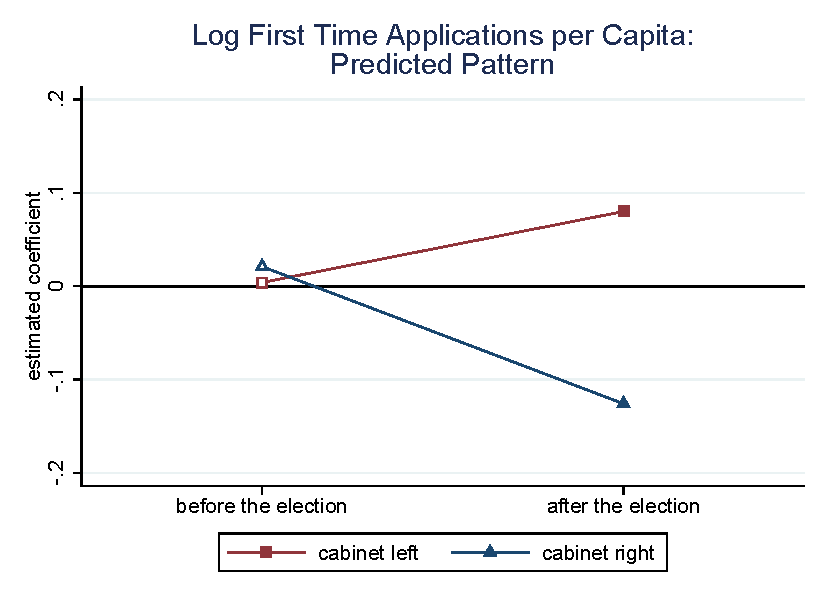
\includegraphics[width=1\textwidth]{figures_edited/app_graph1_R15.pdf}
	\caption{R15: log First Time Asylum Applications per Capita: Predicted Pattern}
\end{figure}

\begin{table}[!ht]\centering
	\renewcommand{\arraystretch}{1.25}
	\def\sym#1{\ifmmode^{#1}\else\(^{#1}\)\fi}
	\caption{R15: Log First Time Applications per Capita: Predicted Pattern}
	\begin{tabular}{l*{2}{c}}
		\hline\hline
		                    &\multicolumn{1}{c}{(1)}&\multicolumn{1}{c}{(2)}\\
                    &\multicolumn{1}{c}{left}&\multicolumn{1}{c}{right}\\
\hline
before              &     0.00401         &      0.0210         \\
                    &    (0.0283)         &    (0.0228)         \\
after               &      0.0799\sym{***}&      -0.125\sym{***}\\
                    &    (0.0229)         &    (0.0238)         \\
\hline
Observations        &       23248         &       23248         \\

		\hline\hline
		\multicolumn{3}{c}{\footnotesize Standard errors in parentheses} \\
		\multicolumn{3}{c}{\footnotesize (\sym{*} \(p<0.05\), \sym{**} \(p<0.01\), \sym{***} \(p<0.001\))}\\
	\end{tabular}
\end{table}

\clearpage
\textbf{R15: Use only 4 quarters around the election - Model 2}
\begin{figure}[!ht]
	\centering
	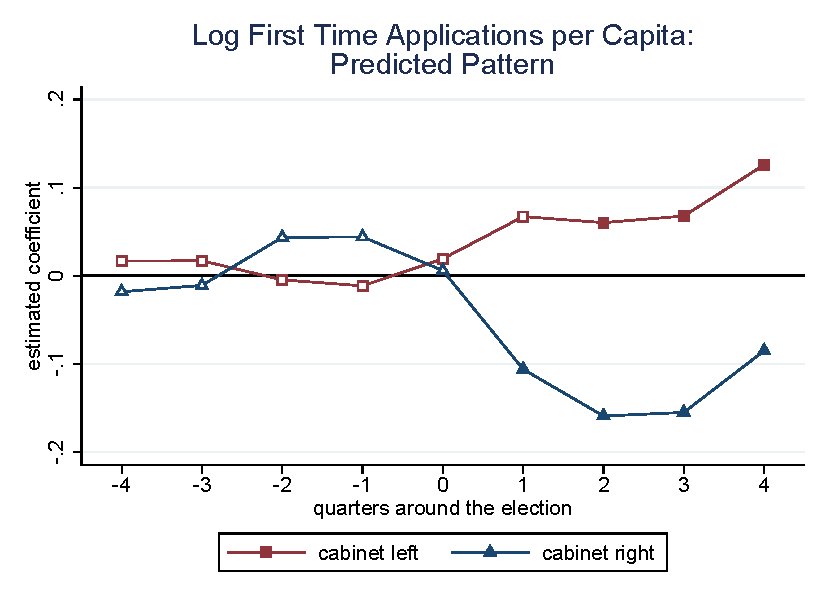
\includegraphics[width=0.7\textwidth]{figures_edited/app_graph2_R15.pdf}
	\caption{R15: log First Time Asylum Applications per Capita: Predicted Pattern}
\end{figure}

\begin{table}[!ht]\centering
	\footnotesize
	\renewcommand{\arraystretch}{1.2}
	\def\sym#1{\ifmmode^{#1}\else\(^{#1}\)\fi}
	\caption{R15: Log First Time Applications per Capita: Predicted Pattern}
	\begin{tabular}{l*{2}{c}}
		\hline\hline
		                    &\multicolumn{1}{c}{(1)}&\multicolumn{1}{c}{(2)}\\
                    &\multicolumn{1}{c}{left}&\multicolumn{1}{c}{right}\\
\hline
 4 quarters before the election&      0.0167         &     -0.0181         \\
                    &    (0.0379)         &    (0.0360)         \\
 3 quarters before the election&      0.0171         &     -0.0109         \\
                    &    (0.0403)         &    (0.0291)         \\
 2 quarters before the election&    -0.00455         &      0.0436         \\
                    &    (0.0312)         &    (0.0377)         \\
 1 quarters before the election&     -0.0114         &      0.0442         \\
                    &    (0.0360)         &    (0.0330)         \\
Quarter of the election&      0.0194         &     0.00599         \\
                    &    (0.0365)         &    (0.0366)         \\
 1 quarters after the election&      0.0672         &      -0.106\sym{***}\\
                    &    (0.0380)         &    (0.0309)         \\
 2 quarters after the election&      0.0603\sym{*}  &      -0.159\sym{***}\\
                    &    (0.0293)         &    (0.0341)         \\
 3 quarters after the election&      0.0679\sym{*}  &      -0.155\sym{***}\\
                    &    (0.0329)         &    (0.0380)         \\
 4 quarters after the election&       0.126\sym{***}&     -0.0851\sym{**} \\
                    &    (0.0276)         &    (0.0325)         \\
\hline
Observations        &       23248         &       23248         \\

		\hline\hline
		\multicolumn{3}{c}{\footnotesize Standard errors in parentheses} \\
		\multicolumn{3}{c}{\footnotesize (\sym{*} \(p<0.05\), \sym{**} \(p<0.01\), \sym{***} \(p<0.001\))} \\
	\end{tabular}
\end{table}



% ===============================================================================================================


\clearpage
\FloatBarrier
\subsection{Do not impute first-time application data for 2008 and 2009}
\begin{table}[!ht]\centering
	\renewcommand{\arraystretch}{1.25}
	\small
	\def\sym#1{\ifmmode^{#1}\else\(^{#1}\)\fi}
	\caption{R16: Determinants of log(First time asylum applications per capita)}
	\begin{tabular}{l*{3}{c}}
		\hline\hline
		                                        &\multicolumn{1}{c}{(1)}         &\multicolumn{1}{c}{(2)}         &\multicolumn{1}{c}{(3)}         \\
\hline
Political Terror Scale                  &     0.426\sym{***}&     0.419\sym{***}&                   \\
                                        &  (0.0723)         &  (0.0716)         &                   \\
Civic Liberty (FHI)                     &     0.182         &     0.184         &                   \\
                                        &   (0.141)         &   (0.140)         &                   \\
Political Rights (FHI)                  &    0.0358         &    0.0389         &                   \\
                                        &  (0.0784)         &  (0.0765)         &                   \\
Quarterly civil war battle death (000s) &     0.124\sym{***}&     0.124\sym{***}&                   \\
                                        &  (0.0141)         &  (0.0139)         &                   \\
Log origin country real GDP per capita  &    -0.620\sym{***}&    -0.642\sym{***}&                   \\
                                        &   (0.169)         &   (0.168)         &                   \\
Log migrant stock in 2000/1             &     0.262\sym{***}&                   &     0.260\sym{***}\\
                                        &  (0.0213)         &                   &  (0.0212)         \\
Log distance from origin to destination &    -0.503         &                   &    -0.527         \\
                                        &   (0.311)         &                   &   (0.311)         \\
Log destination country real GDP per capita&    -1.441\sym{**} &    -1.514\sym{**} &    -1.189\sym{*}  \\
                                        &   (0.498)         &   (0.449)         &   (0.473)         \\
Quarterly unemployment rate at destination&   -0.0694\sym{***}&   -0.0706\sym{***}&   -0.0685\sym{***}\\
                                        &  (0.0117)         &  (0.0110)         &  (0.0118)         \\
Cabinet position left * Before the election&    0.0163         &    0.0148         &   0.00351         \\
                                        &  (0.0292)         &  (0.0292)         &  (0.0310)         \\
Cabinet position left * After the election&     0.110\sym{***}&     0.102\sym{***}&     0.106\sym{***}\\
                                        &  (0.0250)         &  (0.0233)         &  (0.0256)         \\
Cabinet position right * Before the election&    0.0355         &    0.0381         &    0.0381         \\
                                        &  (0.0246)         &  (0.0234)         &  (0.0246)         \\
Cabinet position right * After the election&   -0.0915\sym{**} &   -0.0865\sym{**} &   -0.0981\sym{***}\\
                                        &  (0.0280)         &  (0.0271)         &  (0.0275)         \\
\hline
Observations                            &     22794         &     22794         &     22794         \\
Adjusted \(R^{2}\)                      &     0.437         &     0.176         &     0.442         \\
Fixed Effects                           &         O         &     D x O         &     O x T         \\
Destination dummies                     &       Yes         &        No         &       Yes         \\
Quarter-Year dummies                    &       Yes         &       Yes         &        No         \\

		\hline\hline
		\multicolumn{4}{l}{\footnotesize Standard errors in parentheses (\sym{*} \(p<0.05\), \sym{**} \(p<0.01\), \sym{***} \(p<0.001\))}\\
	\end{tabular}
\end{table}

\clearpage
\textbf{R16: Do not impute first-time application data for 2008 and 2009 - Model 1}
\begin{figure}[!ht]
	\centering
	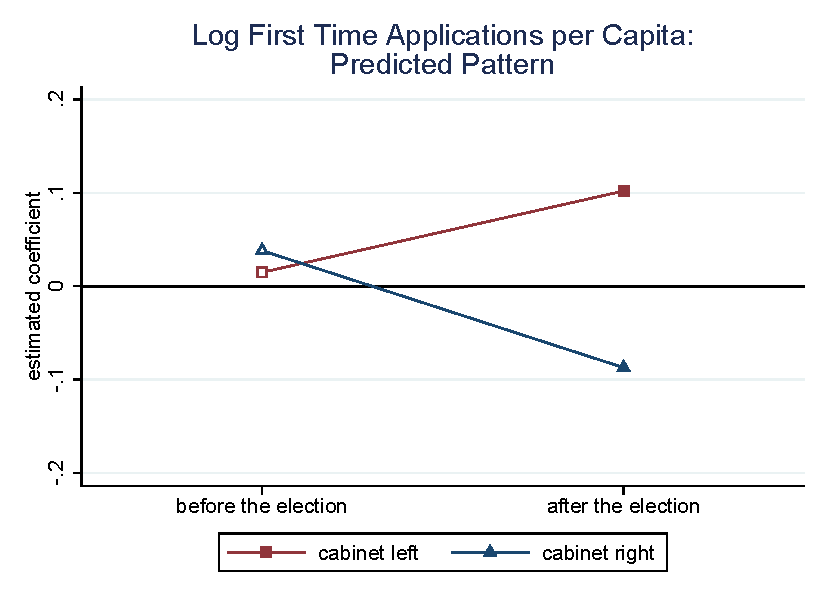
\includegraphics[width=1\textwidth]{figures_edited/app_graph1_R16.pdf}
	\caption{R16: log First Time Asylum Applications per Capita: Predicted Pattern}
\end{figure}

\begin{table}[!ht]\centering
	\renewcommand{\arraystretch}{1.25}
	\def\sym#1{\ifmmode^{#1}\else\(^{#1}\)\fi}
	\caption{R16: Log First Time Applications per Capita: Predicted Pattern}
	\begin{tabular}{l*{2}{c}}
		\hline\hline
		                    &\multicolumn{1}{c}{(1)}&\multicolumn{1}{c}{(2)}\\
                    &\multicolumn{1}{c}{left}&\multicolumn{1}{c}{right}\\
\hline
before              &      0.0149         &      0.0381         \\
                    &    (0.0293)         &    (0.0234)         \\
after               &       0.102\sym{***}&     -0.0872\sym{**} \\
                    &    (0.0233)         &    (0.0270)         \\
\hline
Observations        &       22794         &       22794         \\

		\hline\hline
		\multicolumn{3}{c}{\footnotesize Standard errors in parentheses} \\
		\multicolumn{3}{c}{\footnotesize (\sym{*} \(p<0.05\), \sym{**} \(p<0.01\), \sym{***} \(p<0.001\))}\\
	\end{tabular}
\end{table}

\clearpage
\textbf{R16: Do not impute first-time application data for 2008 and 2009 - Model 2}
\begin{figure}[!ht]
	\centering
	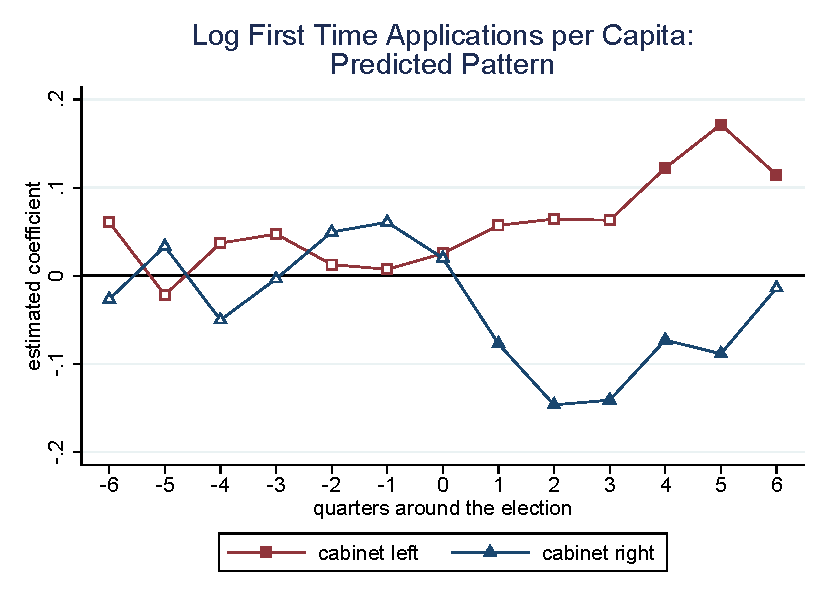
\includegraphics[width=0.7\textwidth]{figures_edited/app_graph2_R16.pdf}
	\caption{R16: log First Time Asylum Applications per Capita: Predicted Pattern}
\end{figure}

\begin{table}[!ht]\centering
	\footnotesize
	\renewcommand{\arraystretch}{1.2}
	\def\sym#1{\ifmmode^{#1}\else\(^{#1}\)\fi}
	\caption{R16: Log First Time Applications per Capita: Predicted Pattern}
	\begin{tabular}{l*{2}{c}}
		\hline\hline
		                    &\multicolumn{1}{c}{(1)}&\multicolumn{1}{c}{(2)}\\
                    &\multicolumn{1}{c}{left}&\multicolumn{1}{c}{right}\\
\hline
 6 quarters before the election&      0.0521         &      0.0549         \\
                    &    (0.0378)         &    (0.0411)         \\
 5 quarters before the election&     -0.0175         &      0.0892\sym{**} \\
                    &    (0.0379)         &    (0.0325)         \\
 4 quarters before the election&      0.0370         &     0.00273         \\
                    &    (0.0394)         &    (0.0376)         \\
 3 quarters before the election&      0.0491         &      0.0148         \\
                    &    (0.0433)         &    (0.0300)         \\
 2 quarters before the election&      0.0185         &      0.0645         \\
                    &    (0.0339)         &    (0.0391)         \\
 1 quarters before the election&     0.00961         &      0.0716\sym{*}  \\
                    &    (0.0384)         &    (0.0352)         \\
Quarter of the election&      0.0373         &      0.0290         \\
                    &    (0.0397)         &    (0.0377)         \\
 1 quarters after the election&      0.0678         &     -0.0709\sym{*}  \\
                    &    (0.0419)         &    (0.0343)         \\
 2 quarters after the election&      0.0765\sym{*}  &      -0.132\sym{***}\\
                    &    (0.0348)         &    (0.0380)         \\
 3 quarters after the election&      0.0728\sym{*}  &      -0.131\sym{**} \\
                    &    (0.0323)         &    (0.0450)         \\
 4 quarters after the election&       0.135\sym{***}&     -0.0491         \\
                    &    (0.0293)         &    (0.0402)         \\
 5 quarters after the election&       0.186\sym{***}&     -0.0733         \\
                    &    (0.0287)         &    (0.0387)         \\
 6 quarters after the election&       0.124\sym{***}&     0.00350         \\
                    &    (0.0320)         &    (0.0333)         \\
\hline
Observations        &       22794         &       22794         \\

		\hline\hline
		\multicolumn{3}{c}{\footnotesize Standard errors in parentheses} \\
		\multicolumn{3}{c}{\footnotesize (\sym{*} \(p<0.05\), \sym{**} \(p<0.01\), \sym{***} \(p<0.001\))} \\
	\end{tabular}
\end{table}




% ===============================================================================================================


\clearpage
\FloatBarrier
\subsection{Include refugee crisis 2015 and 2016}
\begin{table}[!ht]\centering
	\renewcommand{\arraystretch}{1.25}
	\small
	\def\sym#1{\ifmmode^{#1}\else\(^{#1}\)\fi}
	\caption{R17: Determinants of log(First time asylum applications per capita)}
	\begin{tabular}{l*{3}{c}}
		\hline\hline
		                                        &\multicolumn{1}{c}{(1)}         &\multicolumn{1}{c}{(2)}         &\multicolumn{1}{c}{(3)}         \\
\hline
Political Terror Scale                  &     0.407\sym{***}&     0.409\sym{***}&                   \\
                                        &  (0.0755)         &  (0.0757)         &                   \\
Civic Liberty (FHI)                     &     0.182         &     0.181         &                   \\
                                        &   (0.140)         &   (0.139)         &                   \\
Political Rights (FHI)                  & -0.000124         &-0.0000611         &                   \\
                                        &  (0.0752)         &  (0.0746)         &                   \\
Quarterly civil war battle death (000s) &     0.143\sym{***}&     0.142\sym{***}&                   \\
                                        &  (0.0148)         &  (0.0146)         &                   \\
Log origin country real GDP per capita  &    -0.655\sym{***}&    -0.647\sym{***}&                   \\
                                        &   (0.125)         &   (0.123)         &                   \\
Log migrant stock in 2000/1             &     0.253\sym{***}&                   &     0.253\sym{***}\\
                                        &  (0.0223)         &                   &  (0.0223)         \\
Log distance from origin to destination &    -0.679\sym{*}  &                   &    -0.688\sym{*}  \\
                                        &   (0.289)         &                   &   (0.287)         \\
Log destination country real GDP per capita&    -1.675\sym{**} &    -1.836\sym{***}&    -1.424\sym{**} \\
                                        &   (0.488)         &   (0.452)         &   (0.454)         \\
Quarterly unemployment rate at destination&   -0.0739\sym{***}&   -0.0756\sym{***}&   -0.0748\sym{***}\\
                                        &  (0.0128)         &  (0.0125)         &  (0.0132)         \\
Cabinet position left * Before the election&     0.112\sym{***}&     0.114\sym{***}&     0.102\sym{**} \\
                                        &  (0.0282)         &  (0.0275)         &  (0.0298)         \\
Cabinet position left * After the election&     0.131\sym{***}&     0.126\sym{***}&     0.120\sym{***}\\
                                        &  (0.0206)         &  (0.0192)         &  (0.0211)         \\
Cabinet position right * Before the election&   0.00134         &   0.00585         &   0.00524         \\
                                        &  (0.0283)         &  (0.0268)         &  (0.0280)         \\
Cabinet position right * After the election&   -0.0803\sym{**} &   -0.0726\sym{**} &   -0.0853\sym{**} \\
                                        &  (0.0261)         &  (0.0243)         &  (0.0265)         \\
\hline
Observations                            &     24899         &     24899         &     24899         \\
Adjusted \(R^{2}\)                      &     0.451         &     0.176         &     0.453         \\
Fixed Effects                           &         O         &     D x O         &     O x T         \\
Destination dummies                     &       Yes         &        No         &       Yes         \\
Quarter-Year dummies                    &       Yes         &       Yes         &        No         \\

		\hline\hline
		\multicolumn{4}{l}{\footnotesize Standard errors in parentheses (\sym{*} \(p<0.05\), \sym{**} \(p<0.01\), \sym{***} \(p<0.001\))}\\
	\end{tabular}
\end{table}

\clearpage
\textbf{R17: Include refugee crisis 2015 and 2016 - Model 1}
\begin{figure}[!ht]
	\centering
	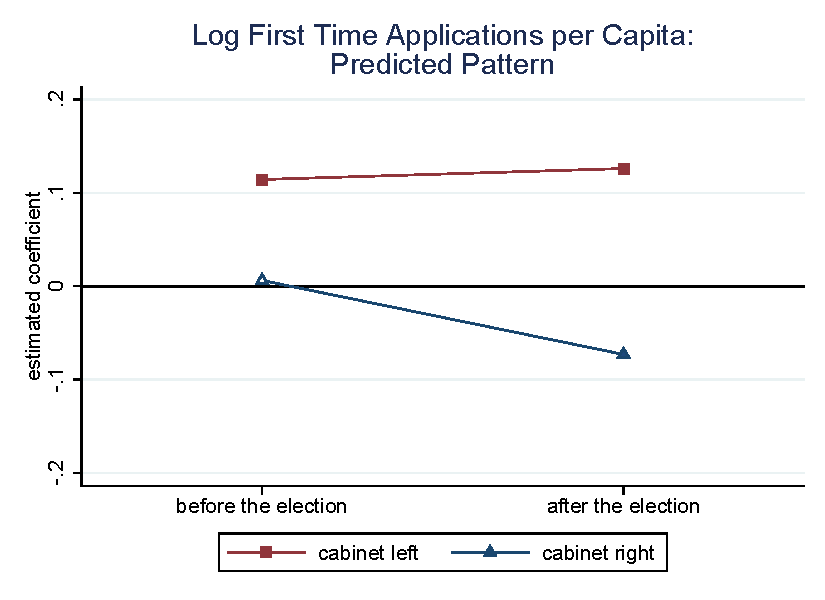
\includegraphics[width=1\textwidth]{figures_edited/app_graph1_R17.pdf}
	\caption{R17: log First Time Asylum Applications per Capita: Predicted Pattern}
\end{figure}

\begin{table}[!ht]\centering
	\renewcommand{\arraystretch}{1.25}
	\def\sym#1{\ifmmode^{#1}\else\(^{#1}\)\fi}
	\caption{R17: Log First Time Applications per Capita: Predicted Pattern}
	\begin{tabular}{l*{2}{c}}
		\hline\hline
		                    &\multicolumn{1}{c}{(1)}&\multicolumn{1}{c}{(2)}\\
                    &\multicolumn{1}{c}{left}&\multicolumn{1}{c}{right}\\
\hline
before              &       0.114\sym{***}&     0.00585         \\
                    &    (0.0275)         &    (0.0268)         \\
after               &       0.126\sym{***}&     -0.0726\sym{**} \\
                    &    (0.0192)         &    (0.0243)         \\
\hline
Observations        &       24899         &       24899         \\

		\hline\hline
		\multicolumn{3}{c}{\footnotesize Standard errors in parentheses} \\
		\multicolumn{3}{c}{\footnotesize (\sym{*} \(p<0.05\), \sym{**} \(p<0.01\), \sym{***} \(p<0.001\))}\\
	\end{tabular}
\end{table}

\clearpage
\textbf{R17: Include refugee crisis 2015 and 2016 - Model 2}
\begin{figure}[!ht]
	\centering
	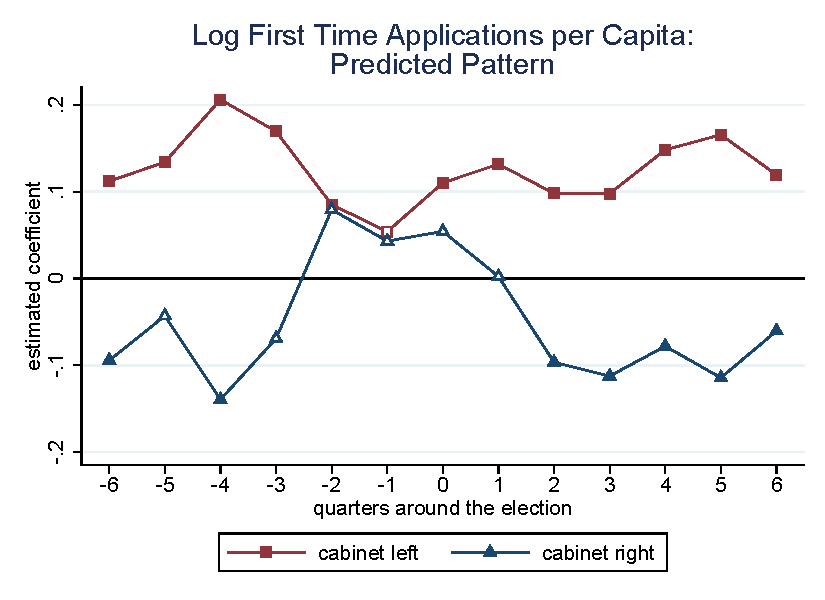
\includegraphics[width=0.7\textwidth]{figures_edited/app_graph2_R17.pdf}
	\caption{R17: log First Time Asylum Applications per Capita: Predicted Pattern}
\end{figure}

\begin{table}[!ht]\centering
	\footnotesize
	\renewcommand{\arraystretch}{1.2}
	\def\sym#1{\ifmmode^{#1}\else\(^{#1}\)\fi}
	\caption{R17: Log First Time Applications per Capita: Predicted Pattern}
	\begin{tabular}{l*{2}{c}}
		\hline\hline
		                    &\multicolumn{1}{c}{(1)}&\multicolumn{1}{c}{(2)}\\
                    &\multicolumn{1}{c}{left}&\multicolumn{1}{c}{right}\\
\hline
 6 quarters before the election&       0.101\sym{**} &     -0.0314         \\
                    &    (0.0336)         &    (0.0421)         \\
 5 quarters before the election&       0.137\sym{***}&    0.000390         \\
                    &    (0.0301)         &    (0.0329)         \\
 4 quarters before the election&       0.199\sym{***}&     -0.0963\sym{**} \\
                    &    (0.0335)         &    (0.0348)         \\
 3 quarters before the election&       0.151\sym{***}&     -0.0593         \\
                    &    (0.0345)         &    (0.0392)         \\
 2 quarters before the election&      0.0778\sym{*}  &      0.0853\sym{*}  \\
                    &    (0.0347)         &    (0.0428)         \\
 1 quarters before the election&      0.0504         &      0.0445         \\
                    &    (0.0415)         &    (0.0412)         \\
Quarter of the election&       0.116\sym{**} &      0.0554         \\
                    &    (0.0387)         &    (0.0362)         \\
 1 quarters after the election&       0.137\sym{***}&    0.000698         \\
                    &    (0.0343)         &    (0.0324)         \\
 2 quarters after the election&       0.103\sym{***}&     -0.0910\sym{**} \\
                    &    (0.0303)         &    (0.0324)         \\
 3 quarters after the election&       0.102\sym{**} &      -0.106\sym{**} \\
                    &    (0.0323)         &    (0.0365)         \\
 4 quarters after the election&       0.153\sym{***}&     -0.0639         \\
                    &    (0.0288)         &    (0.0341)         \\
 5 quarters after the election&       0.172\sym{***}&      -0.108\sym{**} \\
                    &    (0.0260)         &    (0.0338)         \\
 6 quarters after the election&       0.121\sym{***}&     -0.0495\sym{*}  \\
                    &    (0.0269)         &    (0.0248)         \\
\hline
Observations        &       24899         &       24899         \\

		\hline\hline
		\multicolumn{3}{c}{\footnotesize Standard errors in parentheses} \\
		\multicolumn{3}{c}{\footnotesize (\sym{*} \(p<0.05\), \sym{**} \(p<0.01\), \sym{***} \(p<0.001\))} \\
	\end{tabular}
\end{table}




% ===============================================================================================================


\clearpage
\FloatBarrier
\subsection{Use all destination countries with a maximum of two years missing first-time application data}
\begin{table}[!ht]\centering
	\renewcommand{\arraystretch}{1.25}
	\small
	\def\sym#1{\ifmmode^{#1}\else\(^{#1}\)\fi}
	\caption{R18: Determinants of log(First time asylum applications per capita)}
	\begin{tabular}{l*{3}{c}}
		\hline\hline
		                                        &\multicolumn{1}{c}{(1)}         &\multicolumn{1}{c}{(2)}         &\multicolumn{1}{c}{(3)}         \\
\hline
Political Terror Scale                  &     0.381\sym{***}&     0.381\sym{***}&                   \\
                                        &  (0.0710)         &  (0.0704)         &                   \\
Civic Liberty (FHI)                     &     0.132         &     0.130         &                   \\
                                        &   (0.137)         &   (0.136)         &                   \\
Political Rights (FHI)                  &    0.0430         &    0.0443         &                   \\
                                        &  (0.0687)         &  (0.0684)         &                   \\
Quarterly civil war battle death (000s) &     0.190\sym{***}&     0.188\sym{***}&                   \\
                                        &  (0.0223)         &  (0.0221)         &                   \\
Log origin country real GDP per capita  &    -0.614\sym{**} &    -0.611\sym{**} &                   \\
                                        &   (0.189)         &   (0.189)         &                   \\
Log migrant stock in 2000/1             &     0.233\sym{***}&                   &     0.233\sym{***}\\
                                        &  (0.0205)         &                   &  (0.0204)         \\
Log distance from origin to destination &    -0.392         &                   &    -0.393         \\
                                        &   (0.213)         &                   &   (0.212)         \\
Log destination country real GDP per capita&    0.0204         &    0.0389         &   -0.0700         \\
                                        &   (0.837)         &   (0.830)         &   (0.731)         \\
Quarterly unemployment rate at destination&   -0.0595\sym{***}&   -0.0595\sym{***}&   -0.0614\sym{***}\\
                                        &  (0.0127)         &  (0.0120)         &  (0.0116)         \\
Cabinet position left * Before the election&    0.0797\sym{*}  &    0.0804\sym{*}  &    0.0628         \\
                                        &  (0.0305)         &  (0.0310)         &  (0.0316)         \\
Cabinet position left * After the election&     0.140\sym{***}&     0.135\sym{***}&     0.127\sym{***}\\
                                        &  (0.0229)         &  (0.0230)         &  (0.0222)         \\
Cabinet position right * Before the election&    0.0569\sym{**} &    0.0553\sym{**} &    0.0585\sym{**} \\
                                        &  (0.0210)         &  (0.0203)         &  (0.0212)         \\
Cabinet position right * After the election&   -0.0567\sym{*}  &   -0.0528\sym{*}  &   -0.0594\sym{*}  \\
                                        &  (0.0229)         &  (0.0220)         &  (0.0232)         \\
\hline
Observations                            &     26242         &     26242         &     26242         \\
Adjusted \(R^{2}\)                      &     0.451         &     0.138         &     0.459         \\
Fixed Effects                           &         O         &     D x O         &     O x T         \\
Destination dummies                     &       Yes         &        No         &       Yes         \\
Quarter-Year dummies                    &       Yes         &       Yes         &        No         \\

		\hline\hline
		\multicolumn{4}{l}{\footnotesize Standard errors in parentheses (\sym{*} \(p<0.05\), \sym{**} \(p<0.01\), \sym{***} \(p<0.001\))}\\
	\end{tabular}
\end{table}

\clearpage
\textbf{R18: Use all destination countries with a maximum of two years missing first-time application data - Model 1}
\begin{figure}[!ht]
	\centering
	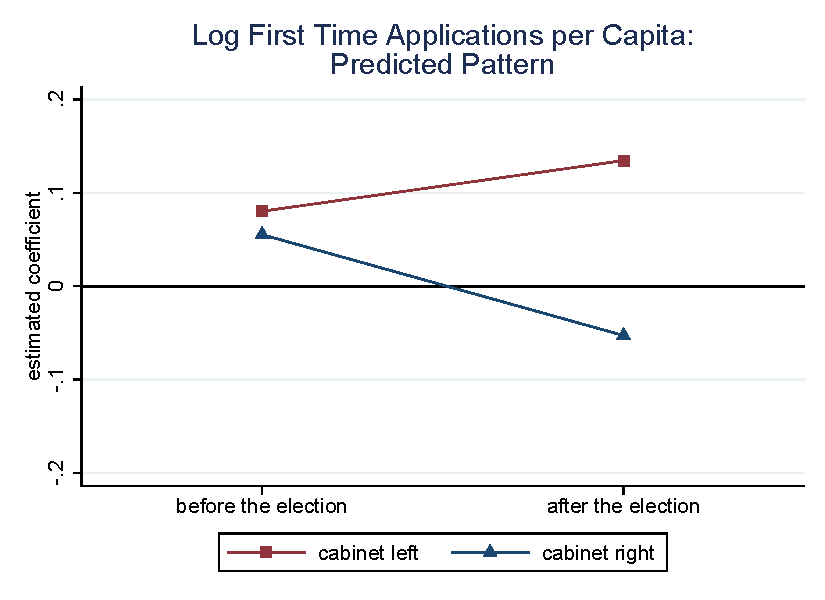
\includegraphics[width=1\textwidth]{figures_edited/app_graph1_R18.pdf}
	\caption{R18: log First Time Asylum Applications per Capita: Predicted Pattern}
\end{figure}

\begin{table}[!ht]\centering
	\renewcommand{\arraystretch}{1.25}
	\def\sym#1{\ifmmode^{#1}\else\(^{#1}\)\fi}
	\caption{R18: Log First Time Applications per Capita: Predicted Pattern}
	\begin{tabular}{l*{2}{c}}
		\hline\hline
		                    &\multicolumn{1}{c}{(1)}&\multicolumn{1}{c}{(2)}\\
                    &\multicolumn{1}{c}{left}&\multicolumn{1}{c}{right}\\
\hline
before              &      0.0804\sym{**} &      0.0553\sym{**} \\
                    &    (0.0310)         &    (0.0203)         \\
after               &       0.135\sym{***}&     -0.0528\sym{*}  \\
                    &    (0.0230)         &    (0.0220)         \\
\hline
Observations        &       26242         &       26242         \\

		\hline\hline
		\multicolumn{3}{c}{\footnotesize Standard errors in parentheses} \\
		\multicolumn{3}{c}{\footnotesize (\sym{*} \(p<0.05\), \sym{**} \(p<0.01\), \sym{***} \(p<0.001\))}\\
	\end{tabular}
\end{table}

\clearpage
\textbf{R18: Use all destination countries with a maximum of two years missing first-time application data - Model 2}
\begin{figure}[!ht]
	\centering
	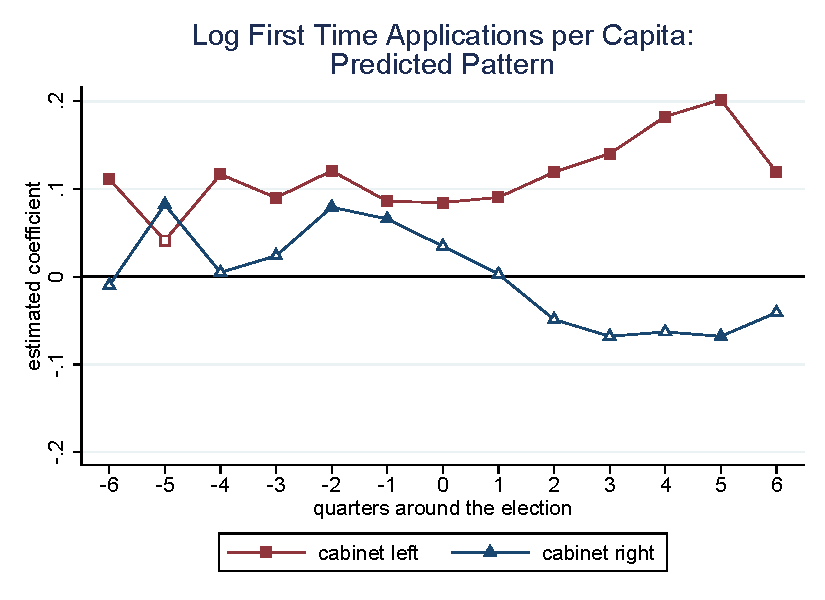
\includegraphics[width=0.7\textwidth]{figures_edited/app_graph2_R18.pdf}
	\caption{R18: log First Time Asylum Applications per Capita: Predicted Pattern}
\end{figure}

\begin{table}[!ht]\centering
	\footnotesize
	\renewcommand{\arraystretch}{1.15}
	\def\sym#1{\ifmmode^{#1}\else\(^{#1}\)\fi}
	\caption{R18: Log First Time Applications per Capita: Predicted Pattern}
	\begin{tabular}{l*{2}{c}}
		\hline\hline
		                    &\multicolumn{1}{c}{(1)}&\multicolumn{1}{c}{(2)}\\
                    &\multicolumn{1}{c}{left}&\multicolumn{1}{c}{right}\\
\hline
 6 quarters before the election&       0.120\sym{**} &      0.0650         \\
                    &    (0.0385)         &    (0.0341)         \\
 5 quarters before the election&      0.0506         &       0.125\sym{***}\\
                    &    (0.0388)         &    (0.0297)         \\
 4 quarters before the election&       0.124\sym{**} &      0.0527         \\
                    &    (0.0411)         &    (0.0374)         \\
 3 quarters before the election&      0.0970\sym{*}  &      0.0389         \\
                    &    (0.0435)         &    (0.0275)         \\
 2 quarters before the election&       0.124\sym{**} &      0.0909\sym{*}  \\
                    &    (0.0413)         &    (0.0359)         \\
 1 quarters before the election&      0.0902\sym{*}  &      0.0729\sym{*}  \\
                    &    (0.0360)         &    (0.0339)         \\
Quarter of the election&      0.0936\sym{*}  &      0.0402         \\
                    &    (0.0387)         &    (0.0339)         \\
 1 quarters after the election&      0.0974\sym{**} &     0.00517         \\
                    &    (0.0374)         &    (0.0306)         \\
 2 quarters after the election&       0.124\sym{***}&     -0.0398         \\
                    &    (0.0331)         &    (0.0356)         \\
 3 quarters after the election&       0.150\sym{***}&     -0.0613         \\
                    &    (0.0379)         &    (0.0349)         \\
 4 quarters after the election&       0.198\sym{***}&     -0.0440         \\
                    &    (0.0315)         &    (0.0344)         \\
 5 quarters after the election&       0.212\sym{***}&     -0.0573         \\
                    &    (0.0240)         &    (0.0347)         \\
 6 quarters after the election&       0.119\sym{***}&     -0.0256         \\
                    &    (0.0314)         &    (0.0273)         \\
\hline
Observations        &       26242         &       26242         \\

		\hline\hline
		\multicolumn{3}{c}{\footnotesize Standard errors in parentheses} \\
		\multicolumn{3}{c}{\footnotesize (\sym{*} \(p<0.05\), \sym{**} \(p<0.01\), \sym{***} \(p<0.001\))} \\
	\end{tabular}
\end{table}




% ===============================================================================================================


\clearpage
\FloatBarrier
\subsection{Use only destination countries that report first-time application data in all years}
\begin{table}[!ht]\centering
	\renewcommand{\arraystretch}{1.25}
	\small
	\def\sym#1{\ifmmode^{#1}\else\(^{#1}\)\fi}
	\caption{R19: Determinants of log(First time asylum applications per capita)}
	\begin{tabular}{l*{3}{c}}
		\hline\hline
		                                        &\multicolumn{1}{c}{(1)}         &\multicolumn{1}{c}{(2)}         &\multicolumn{1}{c}{(3)}         \\
\hline
Political Terror Scale                  &     0.381\sym{***}&     0.381\sym{***}&                   \\
                                        &   (0.106)         &   (0.106)         &                   \\
Civic Liberty (FHI)                     &     0.242         &     0.242         &                   \\
                                        &   (0.136)         &   (0.136)         &                   \\
Political Rights (FHI)                  &   -0.0196         &   -0.0194         &                   \\
                                        &  (0.0645)         &  (0.0644)         &                   \\
Quarterly civil war battle death (000s) &     0.173\sym{***}&     0.173\sym{***}&                   \\
                                        &  (0.0234)         &  (0.0233)         &                   \\
Log origin country real GDP per capita  &    -0.542\sym{*}  &    -0.541\sym{*}  &                   \\
                                        &   (0.207)         &   (0.207)         &                   \\
Log migrant stock in 2000/1             &     0.221\sym{***}&                   &     0.221\sym{***}\\
                                        &  (0.0251)         &                   &  (0.0250)         \\
Log distance from origin to destination &    -0.505         &                   &    -0.505         \\
                                        &   (0.358)         &                   &   (0.358)         \\
Log destination country real GDP per capita&    -1.428         &    -1.464         &    -1.156         \\
                                        &   (0.822)         &   (0.802)         &   (0.670)         \\
Quarterly unemployment rate at destination&   -0.0899\sym{***}&   -0.0893\sym{***}&   -0.0889\sym{***}\\
                                        &  (0.0158)         &  (0.0152)         &  (0.0150)         \\
Cabinet position left * Before the election&     0.157\sym{***}&     0.157\sym{***}&     0.143\sym{***}\\
                                        &  (0.0345)         &  (0.0346)         &  (0.0339)         \\
Cabinet position left * After the election&     0.146\sym{***}&     0.140\sym{***}&     0.135\sym{***}\\
                                        &  (0.0365)         &  (0.0362)         &  (0.0358)         \\
Cabinet position right * Before the election&    0.0550         &    0.0452         &    0.0592         \\
                                        &  (0.0348)         &  (0.0334)         &  (0.0360)         \\
Cabinet position right * After the election&   -0.0580         &   -0.0545         &   -0.0457         \\
                                        &  (0.0401)         &  (0.0376)         &  (0.0384)         \\
\hline
Observations                            &     16128         &     16128         &     16128         \\
Adjusted \(R^{2}\)                      &     0.411         &     0.177         &     0.413         \\
Fixed Effects                           &         O         &     D x O         &     O x T         \\
Destination dummies                     &       Yes         &        No         &       Yes         \\
Quarter-Year dummies                    &       Yes         &       Yes         &        No         \\

		\hline\hline
		\multicolumn{4}{l}{\footnotesize Standard errors in parentheses (\sym{*} \(p<0.05\), \sym{**} \(p<0.01\), \sym{***} \(p<0.001\))}\\
	\end{tabular}
\end{table}

\clearpage
\textbf{R19: Use only destination countries that report first-time application data in all years - Model 1}
\begin{figure}[!ht]
	\centering
	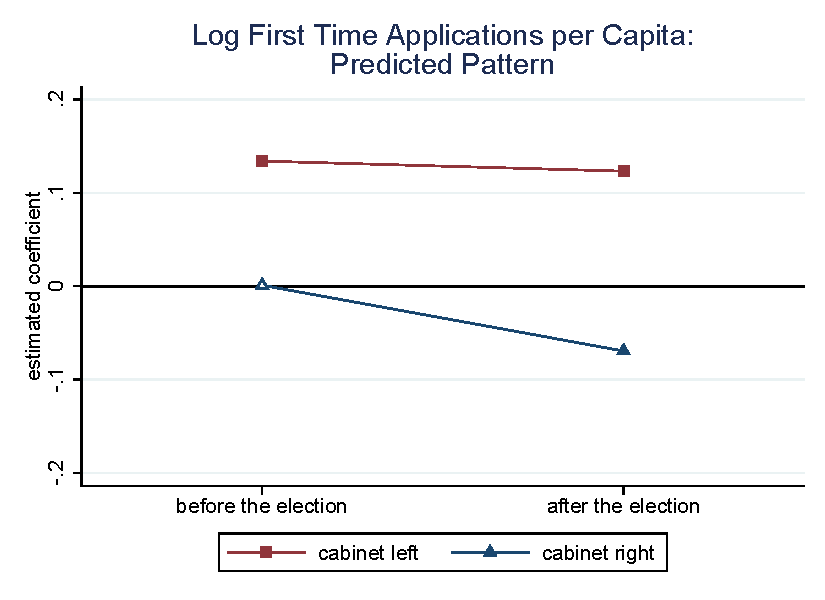
\includegraphics[width=1\textwidth]{figures_edited/app_graph1_R19.pdf}
	\caption{R19: log First Time Asylum Applications per Capita: Predicted Pattern}
\end{figure}

\begin{table}[!ht]\centering
	\renewcommand{\arraystretch}{1.25}
	\def\sym#1{\ifmmode^{#1}\else\(^{#1}\)\fi}
	\caption{R19: Log First Time Applications per Capita: Predicted Pattern}
	\begin{tabular}{l*{2}{c}}
		\hline\hline
		                    &\multicolumn{1}{c}{(1)}&\multicolumn{1}{c}{(2)}\\
                    &\multicolumn{1}{c}{left}&\multicolumn{1}{c}{right}\\
\hline
before              &       0.156\sym{***}&      0.0462         \\
                    &    (0.0346)         &    (0.0336)         \\
after               &       0.141\sym{***}&     -0.0530         \\
                    &    (0.0362)         &    (0.0375)         \\
\hline
Observations        &       16128         &       16128         \\

		\hline\hline
		\multicolumn{3}{c}{\footnotesize Standard errors in parentheses} \\
		\multicolumn{3}{c}{\footnotesize (\sym{*} \(p<0.05\), \sym{**} \(p<0.01\), \sym{***} \(p<0.001\))}\\
	\end{tabular}
\end{table}

\clearpage
\textbf{R19: Use only destination countries that report first-time application data in all years - Model 2}
\begin{figure}[!ht]
	\centering
	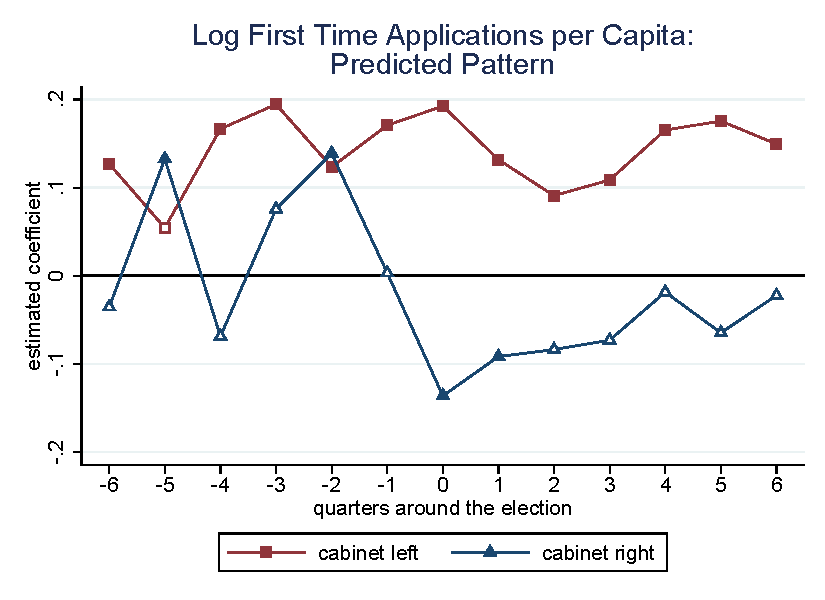
\includegraphics[width=0.7\textwidth]{figures_edited/app_graph2_R19.pdf}
	\caption{R19: log First Time Asylum Applications per Capita: Predicted Pattern}
\end{figure}

\begin{table}[!ht]\centering
	\footnotesize
	\renewcommand{\arraystretch}{1.2}
	\def\sym#1{\ifmmode^{#1}\else\(^{#1}\)\fi}
	\caption{R19: Log First Time Applications per Capita: Predicted Pattern}
	\begin{tabular}{l*{2}{c}}
		\hline\hline
		                    &\multicolumn{1}{c}{(1)}&\multicolumn{1}{c}{(2)}\\
                    &\multicolumn{1}{c}{left}&\multicolumn{1}{c}{right}\\
\hline
 6 quarters before the election&       0.174\sym{***}&       0.139\sym{**} \\
                    &    (0.0431)         &    (0.0489)         \\
 5 quarters before the election&       0.107\sym{*}  &       0.268\sym{***}\\
                    &    (0.0437)         &    (0.0475)         \\
 4 quarters before the election&       0.200\sym{***}&      0.0506         \\
                    &    (0.0445)         &    (0.0620)         \\
 3 quarters before the election&       0.237\sym{***}&       0.106         \\
                    &    (0.0500)         &    (0.0614)         \\
 2 quarters before the election&       0.161\sym{**} &       0.172\sym{**} \\
                    &    (0.0503)         &    (0.0610)         \\
 1 quarters before the election&       0.204\sym{***}&      0.0324         \\
                    &    (0.0486)         &    (0.0408)         \\
Quarter of the election&       0.222\sym{***}&      -0.111\sym{**} \\
                    &    (0.0404)         &    (0.0424)         \\
 1 quarters after the election&       0.162\sym{***}&     -0.0654         \\
                    &    (0.0472)         &    (0.0421)         \\
 2 quarters after the election&       0.124\sym{**} &     -0.0585         \\
                    &    (0.0479)         &    (0.0491)         \\
 3 quarters after the election&       0.138\sym{**} &     -0.0471         \\
                    &    (0.0506)         &    (0.0489)         \\
 4 quarters after the election&       0.191\sym{***}&      0.0112         \\
                    &    (0.0416)         &    (0.0581)         \\
 5 quarters after the election&       0.202\sym{***}&     -0.0341         \\
                    &    (0.0448)         &    (0.0657)         \\
 6 quarters after the election&       0.167\sym{***}&     0.00593         \\
                    &    (0.0457)         &    (0.0478)         \\
\hline
Observations        &       16128         &       16128         \\

		\hline\hline
		\multicolumn{3}{c}{\footnotesize Standard errors in parentheses} \\
		\multicolumn{3}{c}{\footnotesize (\sym{*} \(p<0.05\), \sym{**} \(p<0.01\), \sym{***} \(p<0.001\))} \\
	\end{tabular}
\end{table}



% ===============================================================================================================


\clearpage
\FloatBarrier
\subsection{Add Cyprus to baseline sample of destination countries}
\begin{table}[!ht]\centering
	\renewcommand{\arraystretch}{1.25}
	\small
	\def\sym#1{\ifmmode^{#1}\else\(^{#1}\)\fi}
	\caption{R20: Determinants of log(First time asylum applications per capita)}
	\begin{tabular}{l*{3}{c}}
		\hline\hline
		                                        &\multicolumn{1}{c}{(1)}         &\multicolumn{1}{c}{(2)}         &\multicolumn{1}{c}{(3)}         \\
\hline
Political Terror Scale                  &     0.403\sym{***}&     0.403\sym{***}&                   \\
                                        &  (0.0688)         &  (0.0681)         &                   \\
Civic Liberty (FHI)                     &     0.182         &     0.181         &                   \\
                                        &   (0.140)         &   (0.139)         &                   \\
Political Rights (FHI)                  &    0.0410         &    0.0430         &                   \\
                                        &  (0.0757)         &  (0.0757)         &                   \\
Quarterly civil war battle death (000s) &     0.180\sym{***}&     0.179\sym{***}&                   \\
                                        &  (0.0228)         &  (0.0226)         &                   \\
Log origin country real GDP per capita  &    -0.632\sym{***}&    -0.632\sym{***}&                   \\
                                        &   (0.175)         &   (0.173)         &                   \\
Log migrant stock in 2000/1             &     0.257\sym{***}&                   &     0.257\sym{***}\\
                                        &  (0.0217)         &                   &  (0.0217)         \\
Log distance from origin to destination &    -0.546\sym{*}  &                   &    -0.547\sym{*}  \\
                                        &   (0.221)         &                   &   (0.221)         \\
Log destination country real GDP per capita&    -0.706         &    -0.759         &    -0.533         \\
                                        &   (0.499)         &   (0.473)         &   (0.478)         \\
Quarterly unemployment rate at destination&   -0.0744\sym{***}&   -0.0756\sym{***}&   -0.0716\sym{***}\\
                                        &  (0.0114)         &  (0.0105)         &  (0.0117)         \\
Cabinet position left * Before the election&    0.0827\sym{*}  &    0.0834\sym{*}  &    0.0610         \\
                                        &  (0.0345)         &  (0.0348)         &  (0.0355)         \\
Cabinet position left * After the election&     0.155\sym{***}&     0.147\sym{***}&     0.144\sym{***}\\
                                        &  (0.0236)         &  (0.0233)         &  (0.0233)         \\
Cabinet position right * Before the election&    0.0460\sym{*}  &    0.0467\sym{*}  &    0.0459\sym{*}  \\
                                        &  (0.0227)         &  (0.0211)         &  (0.0228)         \\
Cabinet position right * After the election&   -0.0719\sym{**} &   -0.0670\sym{**} &   -0.0735\sym{**} \\
                                        &  (0.0230)         &  (0.0218)         &  (0.0227)         \\
\hline
Observations                            &     24370         &     24370         &     24370         \\
Adjusted \(R^{2}\)                      &     0.457         &     0.156         &     0.466         \\
Fixed Effects                           &         O         &     D x O         &     O x T         \\
Destination dummies                     &       Yes         &        No         &       Yes         \\
Quarter-Year dummies                    &       Yes         &       Yes         &        No         \\

		\hline\hline
		\multicolumn{4}{l}{\footnotesize Standard errors in parentheses (\sym{*} \(p<0.05\), \sym{**} \(p<0.01\), \sym{***} \(p<0.001\))}\\
	\end{tabular}
\end{table}

\clearpage
\textbf{R20: Add Cyprus to baseline sample of destination countries - Model 1}
\begin{figure}[!ht]
	\centering
	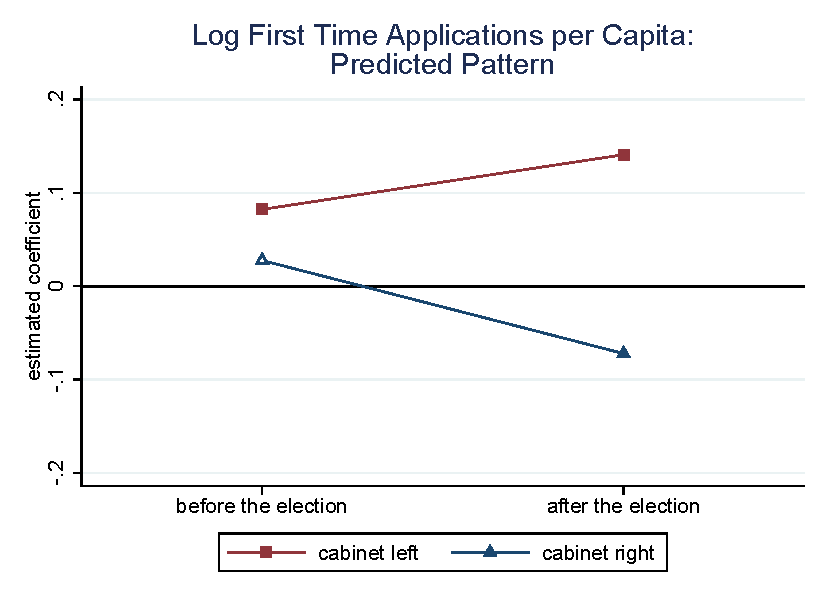
\includegraphics[width=1\textwidth]{figures_edited/app_graph1_R20.pdf}
	\caption{R20: log First Time Asylum Applications per Capita: Predicted Pattern}
\end{figure}

\begin{table}[!ht]\centering
	\renewcommand{\arraystretch}{1.25}
	\def\sym#1{\ifmmode^{#1}\else\(^{#1}\)\fi}
	\caption{R20: Log First Time Applications per Capita: Predicted Pattern}
	\begin{tabular}{l*{2}{c}}
		\hline\hline
		                    &\multicolumn{1}{c}{(1)}&\multicolumn{1}{c}{(2)}\\
                    &\multicolumn{1}{c}{left}&\multicolumn{1}{c}{right}\\
\hline
before              &      0.0834\sym{*}  &      0.0467\sym{*}  \\
                    &    (0.0348)         &    (0.0211)         \\
after               &       0.147\sym{***}&     -0.0664\sym{**} \\
                    &    (0.0233)         &    (0.0219)         \\
\hline
Observations        &       24370         &       24370         \\

		\hline\hline
		\multicolumn{3}{c}{\footnotesize Standard errors in parentheses} \\
		\multicolumn{3}{c}{\footnotesize (\sym{*} \(p<0.05\), \sym{**} \(p<0.01\), \sym{***} \(p<0.001\))}\\
	\end{tabular}
\end{table}

\clearpage
\textbf{R20: Add Cyprus to baseline sample of destination countries - Model 2}
\begin{figure}[!ht]
	\centering
	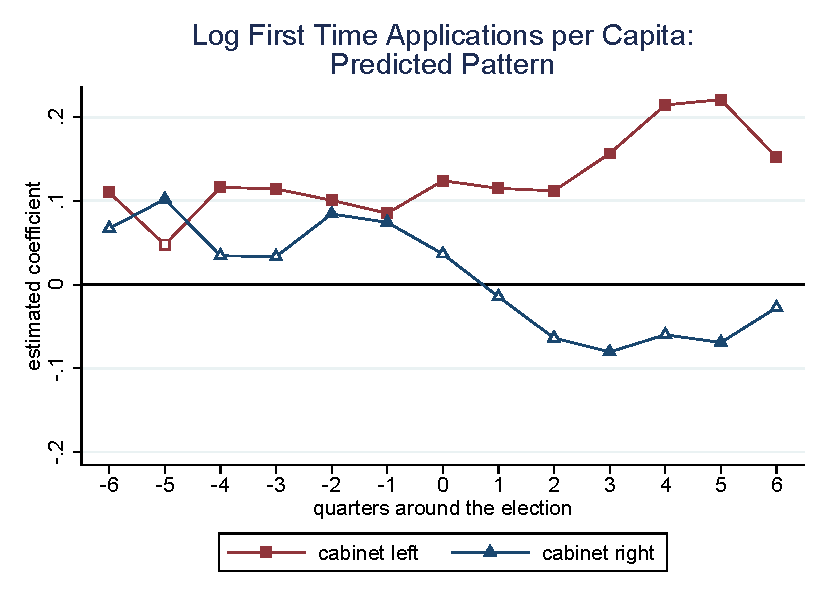
\includegraphics[width=0.7\textwidth]{figures_edited/app_graph2_R20.pdf}
	\caption{R20: log First Time Asylum Applications per Capita: Predicted Pattern}
\end{figure}

\begin{table}[!ht]\centering
	\footnotesize
	\renewcommand{\arraystretch}{1.2}
	\def\sym#1{\ifmmode^{#1}\else\(^{#1}\)\fi}
	\caption{R20: Log First Time Applications per Capita: Predicted Pattern}
	\begin{tabular}{l*{2}{c}}
		\hline\hline
		                    &\multicolumn{1}{c}{(1)}&\multicolumn{1}{c}{(2)}\\
                    &\multicolumn{1}{c}{left}&\multicolumn{1}{c}{right}\\
\hline
 6 quarters before the election&       0.109\sym{**} &      0.0664         \\
                    &    (0.0387)         &    (0.0347)         \\
 5 quarters before the election&      0.0474         &       0.102\sym{***}\\
                    &    (0.0395)         &    (0.0295)         \\
 4 quarters before the election&       0.116\sym{**} &      0.0343         \\
                    &    (0.0423)         &    (0.0359)         \\
 3 quarters before the election&       0.114\sym{*}  &      0.0336         \\
                    &    (0.0472)         &    (0.0291)         \\
 2 quarters before the election&       0.101\sym{*}  &      0.0846\sym{*}  \\
                    &    (0.0429)         &    (0.0384)         \\
 1 quarters before the election&      0.0853\sym{*}  &      0.0744\sym{*}  \\
                    &    (0.0403)         &    (0.0332)         \\
Quarter of the election&       0.124\sym{**} &      0.0366         \\
                    &    (0.0448)         &    (0.0358)         \\
 1 quarters after the election&       0.115\sym{**} &     -0.0143         \\
                    &    (0.0406)         &    (0.0316)         \\
 2 quarters after the election&       0.112\sym{***}&     -0.0633         \\
                    &    (0.0295)         &    (0.0360)         \\
 3 quarters after the election&       0.157\sym{***}&     -0.0798\sym{*}  \\
                    &    (0.0332)         &    (0.0354)         \\
 4 quarters after the election&       0.215\sym{***}&     -0.0592         \\
                    &    (0.0313)         &    (0.0335)         \\
 5 quarters after the election&       0.222\sym{***}&     -0.0687\sym{*}  \\
                    &    (0.0277)         &    (0.0322)         \\
 6 quarters after the election&       0.153\sym{***}&     -0.0273         \\
                    &    (0.0324)         &    (0.0282)         \\
\hline
Observations        &       24370         &       24370         \\

		\hline\hline
		\multicolumn{3}{c}{\footnotesize Standard errors in parentheses} \\
		\multicolumn{3}{c}{\footnotesize (\sym{*} \(p<0.05\), \sym{**} \(p<0.01\), \sym{***} \(p<0.001\))} \\
	\end{tabular}
\end{table}




% ===============================================================================================================


\clearpage
\FloatBarrier
\subsection{Use only countries that are also in baseline decision analysis}
\begin{table}[!ht]\centering
	\renewcommand{\arraystretch}{1.25}
	\small
	\def\sym#1{\ifmmode^{#1}\else\(^{#1}\)\fi}
	\caption{R21: Determinants of log(First time asylum applications per capita)}
	\begin{tabular}{l*{3}{c}}
		\hline\hline
		                                        &\multicolumn{1}{c}{(1)}         &\multicolumn{1}{c}{(2)}         &\multicolumn{1}{c}{(3)}         \\
\hline
Political Terror Scale                  &     0.427\sym{***}&     0.428\sym{***}&                   \\
                                        &  (0.0873)         &  (0.0873)         &                   \\
Civic Liberty (FHI)                     &     0.189         &     0.189         &                   \\
                                        &   (0.147)         &   (0.147)         &                   \\
Political Rights (FHI)                  &    0.0436         &    0.0434         &                   \\
                                        &  (0.0788)         &  (0.0788)         &                   \\
Quarterly civil war battle death (000s) &     0.121\sym{***}&     0.121\sym{***}&                   \\
                                        &  (0.0135)         &  (0.0135)         &                   \\
Log origin country real GDP per capita  &    -0.760\sym{***}&    -0.759\sym{***}&                   \\
                                        &   (0.173)         &   (0.173)         &                   \\
Log migrant stock in 2000/1             &     0.255\sym{***}&                   &     0.255\sym{***}\\
                                        &  (0.0248)         &                   &  (0.0247)         \\
Log distance from origin to destination &    -0.735\sym{*}  &                   &    -0.735\sym{*}  \\
                                        &   (0.301)         &                   &   (0.300)         \\
Log destination country real GDP per capita&    -1.684\sym{**} &    -1.786\sym{***}&    -1.225\sym{*}  \\
                                        &   (0.510)         &   (0.473)         &   (0.498)         \\
Quarterly unemployment rate at destination&   -0.0720\sym{***}&   -0.0732\sym{***}&   -0.0695\sym{***}\\
                                        &  (0.0117)         &  (0.0114)         &  (0.0120)         \\
Cabinet position left * Before the election&    0.0482         &    0.0478         &    0.0468         \\
                                        &  (0.0340)         &  (0.0343)         &  (0.0363)         \\
Cabinet position left * After the election&     0.218\sym{***}&     0.205\sym{***}&     0.220\sym{***}\\
                                        &  (0.0357)         &  (0.0336)         &  (0.0368)         \\
Cabinet position right * Before the election&    0.0659\sym{*}  &    0.0688\sym{*}  &    0.0700\sym{*}  \\
                                        &  (0.0303)         &  (0.0300)         &  (0.0305)         \\
Cabinet position right * After the election&   -0.0415         &   -0.0308         &   -0.0389         \\
                                        &  (0.0343)         &  (0.0324)         &  (0.0332)         \\
\hline
Observations                            &     16176         &     16176         &     16176         \\
Adjusted \(R^{2}\)                      &     0.464         &     0.184         &     0.471         \\
Fixed Effects                           &         O         &     D x O         &     O x T         \\
Destination dummies                     &       Yes         &        No         &       Yes         \\
Quarter-Year dummies                    &       Yes         &       Yes         &        No         \\

		\hline\hline
		\multicolumn{4}{l}{\footnotesize Standard errors in parentheses (\sym{*} \(p<0.05\), \sym{**} \(p<0.01\), \sym{***} \(p<0.001\))}\\
	\end{tabular}
\end{table}

\clearpage
\textbf{R21: Use only countries that are also in baseline decision analysis - Model 1}
\begin{figure}[!ht]
	\centering
	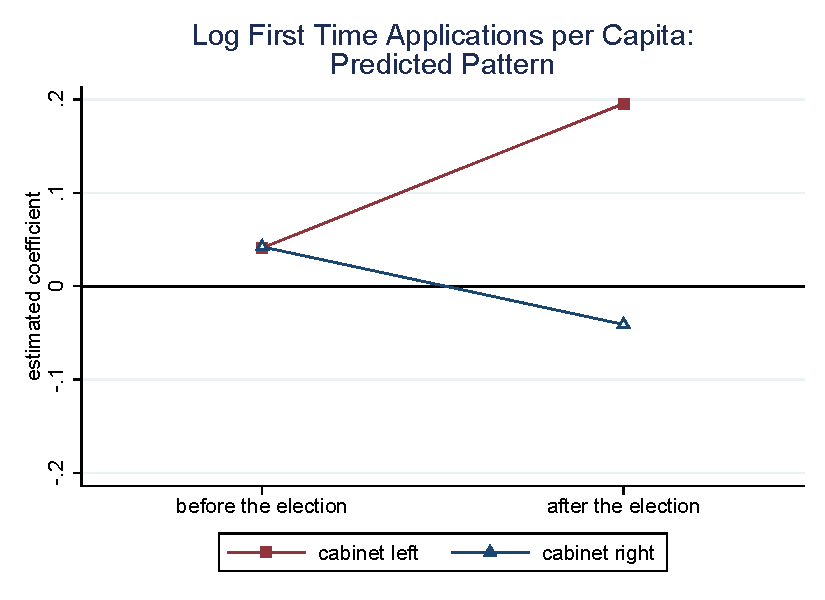
\includegraphics[width=1\textwidth]{figures_edited/app_graph1_R21.pdf}
	\caption{R21: log First Time Asylum Applications per Capita: Predicted Pattern}
\end{figure}

\begin{table}[!ht]\centering
	\renewcommand{\arraystretch}{1.25}
	\def\sym#1{\ifmmode^{#1}\else\(^{#1}\)\fi}
	\caption{R21: Log First Time Applications per Capita: Predicted Pattern}
	\begin{tabular}{l*{2}{c}}
		\hline\hline
		                    &\multicolumn{1}{c}{(1)}&\multicolumn{1}{c}{(2)}\\
                    &\multicolumn{1}{c}{left}&\multicolumn{1}{c}{right}\\
\hline
before              &      0.0480         &      0.0687\sym{*}  \\
                    &    (0.0345)         &    (0.0300)         \\
after               &       0.204\sym{***}&     -0.0309         \\
                    &    (0.0336)         &    (0.0324)         \\
\hline
Observations        &       16176         &       16176         \\

		\hline\hline
		\multicolumn{3}{c}{\footnotesize Standard errors in parentheses} \\
		\multicolumn{3}{c}{\footnotesize (\sym{*} \(p<0.05\), \sym{**} \(p<0.01\), \sym{***} \(p<0.001\))}\\
	\end{tabular}
\end{table}

\clearpage
\textbf{R21: Use only countries that are also in baseline decision analysis - Model 2}
\begin{figure}[!ht]
	\centering
	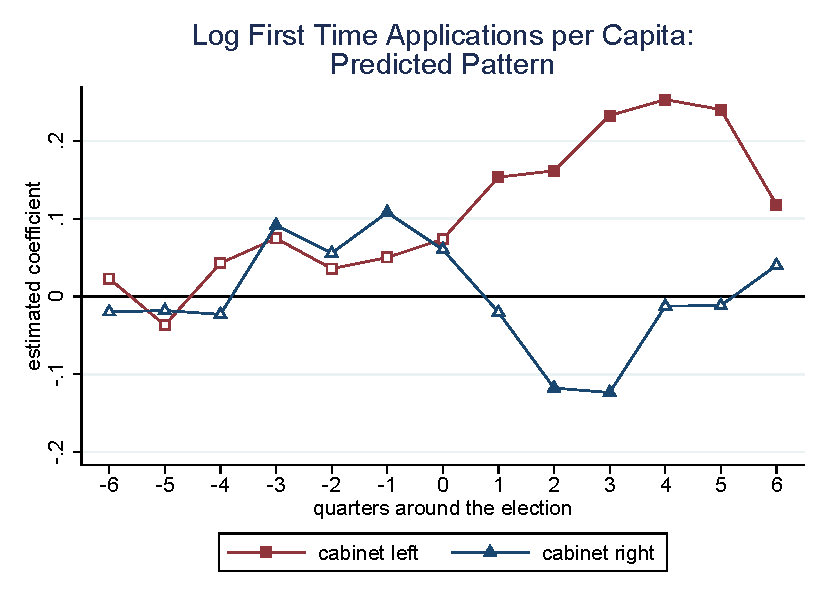
\includegraphics[width=0.7\textwidth]{figures_edited/app_graph2_R21.pdf}
	\caption{R21: log First Time Asylum Applications per Capita: Predicted Pattern}
\end{figure}

\begin{table}[!ht]\centering
	\footnotesize
	\renewcommand{\arraystretch}{1.2}
	\def\sym#1{\ifmmode^{#1}\else\(^{#1}\)\fi}
	\caption{R21: Log First Time Applications per Capita: Predicted Pattern}
	\begin{tabular}{l*{2}{c}}
		\hline\hline
		                    &\multicolumn{1}{c}{(1)}&\multicolumn{1}{c}{(2)}\\
                    &\multicolumn{1}{c}{left}&\multicolumn{1}{c}{right}\\
\hline
 6 quarters before the election&      0.0389         &      0.0906\sym{*}  \\
                    &    (0.0499)         &    (0.0447)         \\
 5 quarters before the election&    -0.00856         &      0.0528         \\
                    &    (0.0509)         &    (0.0346)         \\
 4 quarters before the election&      0.0576         &      0.0494         \\
                    &    (0.0522)         &    (0.0412)         \\
 3 quarters before the election&      0.0877         &       0.114\sym{**} \\
                    &    (0.0492)         &    (0.0361)         \\
 2 quarters before the election&      0.0543         &      0.0789         \\
                    &    (0.0425)         &    (0.0461)         \\
 1 quarters before the election&      0.0679         &       0.122\sym{*}  \\
                    &    (0.0486)         &    (0.0501)         \\
Quarter of the election&      0.0995\sym{*}  &      0.0758         \\
                    &    (0.0478)         &    (0.0519)         \\
 1 quarters after the election&       0.177\sym{***}&     0.00180         \\
                    &    (0.0439)         &    (0.0379)         \\
 2 quarters after the election&       0.184\sym{***}&     -0.0931         \\
                    &    (0.0431)         &    (0.0475)         \\
 3 quarters after the election&       0.253\sym{***}&      -0.103\sym{*}  \\
                    &    (0.0466)         &    (0.0439)         \\
 4 quarters after the election&       0.273\sym{***}&      0.0154         \\
                    &    (0.0373)         &    (0.0424)         \\
 5 quarters after the election&       0.262\sym{***}&     0.00886         \\
                    &    (0.0421)         &    (0.0499)         \\
 6 quarters after the election&       0.136\sym{**} &      0.0655         \\
                    &    (0.0450)         &    (0.0390)         \\
\hline
Observations        &       16176         &       16176         \\

		\hline\hline
		\multicolumn{3}{c}{\footnotesize Standard errors in parentheses} \\
		\multicolumn{3}{c}{\footnotesize (\sym{*} \(p<0.05\), \sym{**} \(p<0.01\), \sym{***} \(p<0.001\))} \\
	\end{tabular}
\end{table}


% ===============================================================================================================


\clearpage
\FloatBarrier
\subsection{Use only countries with a maximum of one early elections}
\begin{table}[!ht]\centering
	\renewcommand{\arraystretch}{1.25}
	\small
	\def\sym#1{\ifmmode^{#1}\else\(^{#1}\)\fi}
	\caption{R22: Determinants of log(First time asylum applications per capita)}
	\begin{tabular}{l*{3}{c}}
		\hline\hline
		                                        &\multicolumn{1}{c}{(1)}         &\multicolumn{1}{c}{(2)}         &\multicolumn{1}{c}{(3)}         \\
\hline
Political Terror Scale                  &     0.395\sym{***}&     0.394\sym{***}&                   \\
                                        &  (0.0741)         &  (0.0735)         &                   \\
Civic Liberty (FHI)                     &     0.176         &     0.176         &                   \\
                                        &   (0.140)         &   (0.138)         &                   \\
Political Rights (FHI)                  &    0.0355         &    0.0369         &                   \\
                                        &  (0.0851)         &  (0.0853)         &                   \\
Quarterly civil war battle death (000s) &     0.188\sym{***}&     0.185\sym{***}&                   \\
                                        &  (0.0232)         &  (0.0230)         &                   \\
Log origin country real GDP per capita  &    -0.710\sym{***}&    -0.713\sym{***}&                   \\
                                        &   (0.166)         &   (0.162)         &                   \\
Log migrant stock in 2000/1             &     0.254\sym{***}&                   &     0.254\sym{***}\\
                                        &  (0.0223)         &                   &  (0.0223)         \\
Log distance from origin to destination &    -0.668\sym{*}  &                   &    -0.679\sym{*}  \\
                                        &   (0.297)         &                   &   (0.295)         \\
Log destination country real GDP per capita&    -1.165\sym{*}  &    -1.245\sym{**} &    -0.872         \\
                                        &   (0.500)         &   (0.463)         &   (0.495)         \\
Quarterly unemployment rate at destination&   -0.0714\sym{***}&   -0.0725\sym{***}&   -0.0700\sym{***}\\
                                        &  (0.0114)         &  (0.0108)         &  (0.0117)         \\
Cabinet position left * Before the election&   -0.0257         &   -0.0272         &   -0.0299         \\
                                        &  (0.0280)         &  (0.0279)         &  (0.0280)         \\
Cabinet position left * After the election&     0.111\sym{***}&    0.0991\sym{***}&     0.111\sym{***}\\
                                        &  (0.0258)         &  (0.0235)         &  (0.0257)         \\
Cabinet position right * Before the election&    0.0122         &    0.0154         &    0.0178         \\
                                        &  (0.0251)         &  (0.0232)         &  (0.0253)         \\
Cabinet position right * After the election&   -0.0374         &   -0.0315         &   -0.0439         \\
                                        &  (0.0277)         &  (0.0266)         &  (0.0288)         \\
\hline
Observations                            &     19293         &     19293         &     19293         \\
Adjusted \(R^{2}\)                      &     0.470         &     0.176         &     0.480         \\
Fixed Effects                           &         O         &     D x O         &     O x T         \\
Destination dummies                     &       Yes         &        No         &       Yes         \\
Quarter-Year dummies                    &       Yes         &       Yes         &        No         \\

		\hline\hline
		\multicolumn{4}{l}{\footnotesize Standard errors in parentheses (\sym{*} \(p<0.05\), \sym{**} \(p<0.01\), \sym{***} \(p<0.001\))}\\
	\end{tabular}
\end{table}

\clearpage
\textbf{R22: Use only countries with a maximum of one early elections - Model 1}
\begin{figure}[!ht]
	\centering
	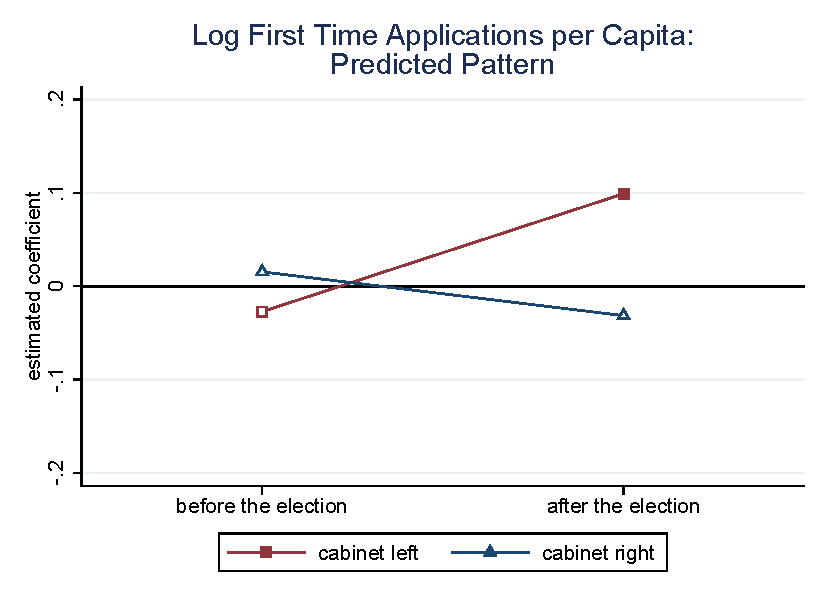
\includegraphics[width=1\textwidth]{figures_edited/app_graph1_R22.pdf}
	\caption{R22: log First Time Asylum Applications per Capita: Predicted Pattern}
\end{figure}

\begin{table}[!ht]\centering
	\renewcommand{\arraystretch}{1.25}
	\def\sym#1{\ifmmode^{#1}\else\(^{#1}\)\fi}
	\caption{R22: Log First Time Applications per Capita: Predicted Pattern}
	\begin{tabular}{l*{2}{c}}
		\hline\hline
		                    &\multicolumn{1}{c}{(1)}&\multicolumn{1}{c}{(2)}\\
                    &\multicolumn{1}{c}{left}&\multicolumn{1}{c}{right}\\
\hline
before              &     -0.0272         &      0.0154         \\
                    &    (0.0279)         &    (0.0232)         \\
after               &      0.0991\sym{***}&     -0.0315         \\
                    &    (0.0235)         &    (0.0266)         \\
\hline
Observations        &       19293         &       19293         \\

		\hline\hline
		\multicolumn{3}{c}{\footnotesize Standard errors in parentheses} \\
		\multicolumn{3}{c}{\footnotesize (\sym{*} \(p<0.05\), \sym{**} \(p<0.01\), \sym{***} \(p<0.001\))}\\
	\end{tabular}
\end{table}

\clearpage
\textbf{R22: Use only countries with a maximum of one early elections - Model 2}
\begin{figure}[!ht]
	\centering
	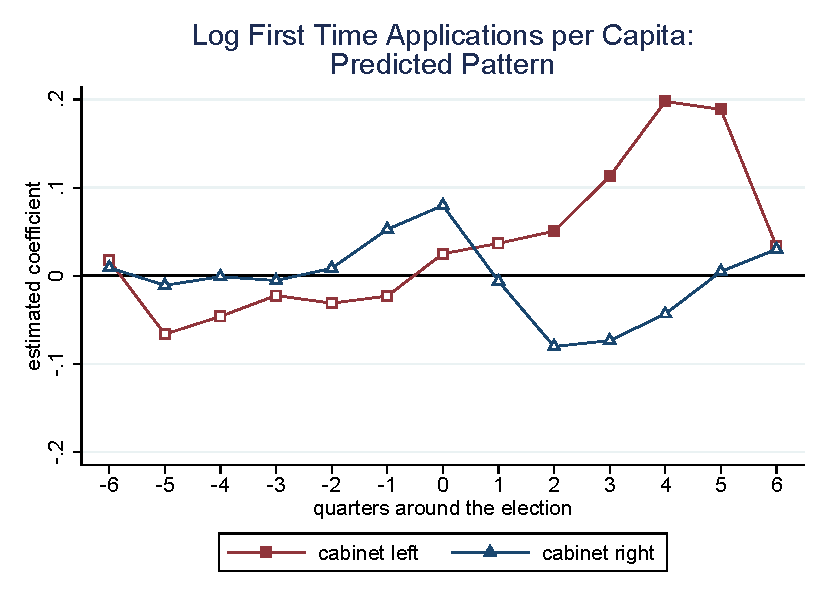
\includegraphics[width=0.7\textwidth]{figures_edited/app_graph2_R22.pdf}
	\caption{R22: log First Time Asylum Applications per Capita: Predicted Pattern}
\end{figure}

\begin{table}[!ht]\centering
	\footnotesize
	\renewcommand{\arraystretch}{1.2}
	\def\sym#1{\ifmmode^{#1}\else\(^{#1}\)\fi}
	\caption{R22: Log First Time Applications per Capita: Predicted Pattern}
	\begin{tabular}{l*{2}{c}}
		\hline\hline
		                    &\multicolumn{1}{c}{(1)}&\multicolumn{1}{c}{(2)}\\
                    &\multicolumn{1}{c}{left}&\multicolumn{1}{c}{right}\\
\hline
 6 quarters before the election&      0.0175         &     0.00926         \\
                    &    (0.0332)         &    (0.0353)         \\
 5 quarters before the election&     -0.0662         &     -0.0108         \\
                    &    (0.0340)         &    (0.0317)         \\
 4 quarters before the election&     -0.0460         &   -0.000948         \\
                    &    (0.0386)         &    (0.0360)         \\
 3 quarters before the election&     -0.0223         &    -0.00538         \\
                    &    (0.0464)         &    (0.0308)         \\
 2 quarters before the election&     -0.0310         &     0.00856         \\
                    &    (0.0333)         &    (0.0371)         \\
 1 quarters before the election&     -0.0229         &      0.0527         \\
                    &    (0.0387)         &    (0.0438)         \\
Quarter of the election&      0.0250         &      0.0798         \\
                    &    (0.0381)         &    (0.0467)         \\
 1 quarters after the election&      0.0369         &    -0.00607         \\
                    &    (0.0383)         &    (0.0352)         \\
 2 quarters after the election&      0.0507         &     -0.0802         \\
                    &    (0.0336)         &    (0.0479)         \\
 3 quarters after the election&       0.113\sym{**} &     -0.0735         \\
                    &    (0.0364)         &    (0.0430)         \\
 4 quarters after the election&       0.198\sym{***}&     -0.0432         \\
                    &    (0.0359)         &    (0.0378)         \\
 5 quarters after the election&       0.189\sym{***}&     0.00484         \\
                    &    (0.0286)         &    (0.0364)         \\
 6 quarters after the election&      0.0336         &      0.0301         \\
                    &    (0.0346)         &    (0.0334)         \\
\hline
Observations        &       19293         &       19293         \\

		\hline\hline
		\multicolumn{3}{c}{\footnotesize Standard errors in parentheses} \\
		\multicolumn{3}{c}{\footnotesize (\sym{*} \(p<0.05\), \sym{**} \(p<0.01\), \sym{***} \(p<0.001\))} \\
	\end{tabular}
\end{table}



% ===============================================================================================================


\clearpage
\FloatBarrier
\subsection{Use only countries with no early elections}
\begin{table}[!ht]\centering
	\renewcommand{\arraystretch}{1.25}
	\small
	\def\sym#1{\ifmmode^{#1}\else\(^{#1}\)\fi}
	\caption{R23: Determinants of log(First time asylum applications per capita)}
	\begin{tabular}{l*{3}{c}}
		\hline\hline
		                                        &\multicolumn{1}{c}{(1)}         &\multicolumn{1}{c}{(2)}         &\multicolumn{1}{c}{(3)}         \\
\hline
Political Terror Scale                  &     0.348\sym{***}&     0.351\sym{***}&                   \\
                                        &  (0.0894)         &  (0.0879)         &                   \\
Civic Liberty (FHI)                     &     0.334\sym{*}  &     0.321\sym{*}  &                   \\
                                        &   (0.136)         &   (0.135)         &                   \\
Political Rights (FHI)                  &   -0.0990         &   -0.0959         &                   \\
                                        &  (0.0747)         &  (0.0771)         &                   \\
Quarterly civil war battle death (000s) &     0.173\sym{***}&     0.170\sym{***}&                   \\
                                        &  (0.0232)         &  (0.0228)         &                   \\
Log origin country real GDP per capita  &    -0.687\sym{***}&    -0.691\sym{***}&                   \\
                                        &   (0.194)         &   (0.186)         &                   \\
Log migrant stock in 2000/1             &     0.270\sym{***}&                   &     0.268\sym{***}\\
                                        &  (0.0334)         &                   &  (0.0332)         \\
Log distance from origin to destination &    -0.909         &                   &    -0.916         \\
                                        &   (0.718)         &                   &   (0.715)         \\
Log destination country real GDP per capita&     1.725\sym{***}&     1.608\sym{**} &     1.702\sym{**} \\
                                        &   (0.475)         &   (0.473)         &   (0.491)         \\
Quarterly unemployment rate at destination&    -0.153\sym{***}&    -0.156\sym{***}&    -0.155\sym{***}\\
                                        &  (0.0225)         &  (0.0199)         &  (0.0244)         \\
Cabinet position left * Before the election&    0.0246         &    0.0167         &    0.0193         \\
                                        &  (0.0342)         &  (0.0318)         &  (0.0323)         \\
Cabinet position left * After the election&     0.106\sym{**} &    0.0812\sym{*}  &     0.102\sym{**} \\
                                        &  (0.0382)         &  (0.0355)         &  (0.0376)         \\
Cabinet position right * Before the election&    0.0233         &    0.0311         &    0.0361         \\
                                        &  (0.0388)         &  (0.0341)         &  (0.0390)         \\
Cabinet position right * After the election&    -0.219\sym{***}&    -0.201\sym{***}&    -0.211\sym{***}\\
                                        &  (0.0380)         &  (0.0355)         &  (0.0385)         \\
\hline
Observations                            &     10974         &     10974         &     10974         \\
Adjusted \(R^{2}\)                      &     0.334         &     0.210         &     0.338         \\
Fixed Effects                           &         O         &     D x O         &     O x T         \\
Destination dummies                     &       Yes         &        No         &       Yes         \\
Quarter-Year dummies                    &       Yes         &       Yes         &        No         \\

		\hline\hline
		\multicolumn{4}{l}{\footnotesize Standard errors in parentheses (\sym{*} \(p<0.05\), \sym{**} \(p<0.01\), \sym{***} \(p<0.001\))}\\
	\end{tabular}
\end{table}

\clearpage
\textbf{R23: Use only countries with no early elections - Model 1}
\begin{figure}[!ht]
	\centering
	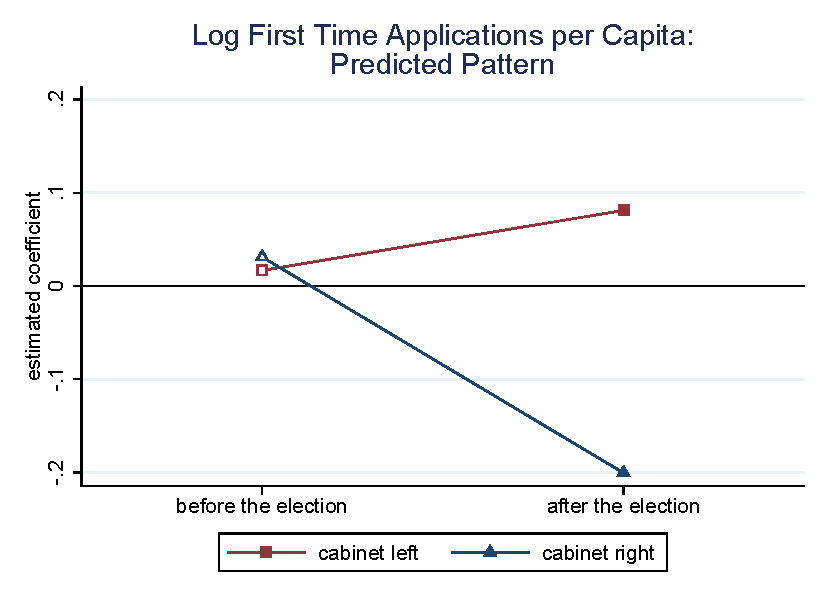
\includegraphics[width=1\textwidth]{figures_edited/app_graph1_R23.pdf}
	\caption{R23: log First Time Asylum Applications per Capita: Predicted Pattern}
\end{figure}

\begin{table}[!ht]\centering
	\renewcommand{\arraystretch}{1.25}
	\def\sym#1{\ifmmode^{#1}\else\(^{#1}\)\fi}
	\caption{R23: Log First Time Applications per Capita: Predicted Pattern}
	\begin{tabular}{l*{2}{c}}
		\hline\hline
		                    &\multicolumn{1}{c}{(1)}&\multicolumn{1}{c}{(2)}\\
                    &\multicolumn{1}{c}{left}&\multicolumn{1}{c}{right}\\
\hline
before              &      0.0167         &      0.0311         \\
                    &    (0.0318)         &    (0.0341)         \\
after               &      0.0812\sym{*}  &      -0.201\sym{***}\\
                    &    (0.0355)         &    (0.0355)         \\
\hline
Observations        &       10974         &       10974         \\

		\hline\hline
		\multicolumn{3}{c}{\footnotesize Standard errors in parentheses} \\
		\multicolumn{3}{c}{\footnotesize (\sym{*} \(p<0.05\), \sym{**} \(p<0.01\), \sym{***} \(p<0.001\))}\\
	\end{tabular}
\end{table}

\clearpage
\textbf{R23: Use only countries with no early elections - Model 2}
\begin{figure}[!ht]
	\centering
	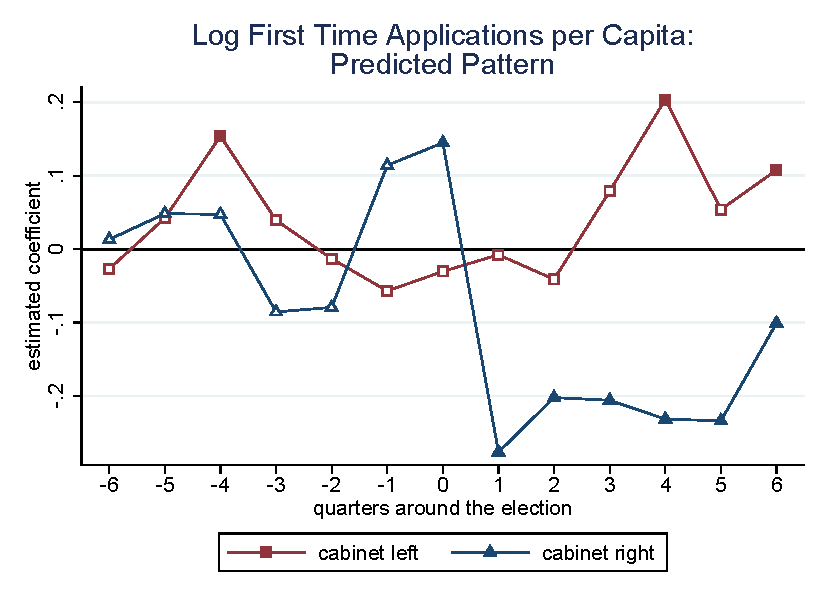
\includegraphics[width=0.7\textwidth]{figures_edited/app_graph2_R23.pdf}
	\caption{R23: log First Time Asylum Applications per Capita: Predicted Pattern}
\end{figure}

\begin{table}[!ht]\centering
	\footnotesize
	\renewcommand{\arraystretch}{1.2}
	\def\sym#1{\ifmmode^{#1}\else\(^{#1}\)\fi}
	\caption{R23: Log First Time Applications per Capita: Predicted Pattern}
	\begin{tabular}{l*{2}{c}}
		\hline\hline
		                    &\multicolumn{1}{c}{(1)}&\multicolumn{1}{c}{(2)}\\
                    &\multicolumn{1}{c}{left}&\multicolumn{1}{c}{right}\\
\hline
 6 quarters before the election&     -0.0295         &      0.0114         \\
                    &    (0.0486)         &    (0.0436)         \\
 5 quarters before the election&      0.0398         &      0.0495         \\
                    &    (0.0426)         &    (0.0427)         \\
 4 quarters before the election&       0.151\sym{**} &      0.0470         \\
                    &    (0.0567)         &    (0.0446)         \\
 3 quarters before the election&      0.0404         &     -0.0850         \\
                    &    (0.0618)         &    (0.0503)         \\
 2 quarters before the election&     -0.0133         &     -0.0849         \\
                    &    (0.0441)         &    (0.0578)         \\
 1 quarters before the election&     -0.0602         &       0.108         \\
                    &    (0.0575)         &    (0.0606)         \\
Quarter of the election&     -0.0366         &       0.130\sym{*}  \\
                    &    (0.0533)         &    (0.0627)         \\
 1 quarters after the election&     -0.0102         &      -0.284\sym{***}\\
                    &    (0.0507)         &    (0.0644)         \\
 2 quarters after the election&     -0.0377         &      -0.211\sym{***}\\
                    &    (0.0515)         &    (0.0585)         \\
 3 quarters after the election&      0.0809         &      -0.211\sym{***}\\
                    &    (0.0566)         &    (0.0536)         \\
 4 quarters after the election&       0.204\sym{***}&      -0.238\sym{***}\\
                    &    (0.0464)         &    (0.0486)         \\
 5 quarters after the election&      0.0571         &      -0.238\sym{***}\\
                    &    (0.0445)         &    (0.0513)         \\
 6 quarters after the election&       0.109\sym{*}  &      -0.103\sym{**} \\
                    &    (0.0482)         &    (0.0356)         \\
\hline
Observations        &       10974         &       10974         \\

		\hline\hline
		\multicolumn{3}{c}{\footnotesize Standard errors in parentheses} \\
		\multicolumn{3}{c}{\footnotesize (\sym{*} \(p<0.05\), \sym{**} \(p<0.01\), \sym{***} \(p<0.001\))} \\
	\end{tabular}
\end{table}




\clearpage
\FloatBarrier
\section{Heterogeneity by origin country region}
\begin{table}[!ht]\centering
	\renewcommand{\arraystretch}{1.25}
	\small
	\def\sym#1{\ifmmode^{#1}\else\(^{#1}\)\fi}
	\caption{Determinants of log(First time asylum applications per capita)}
	\begin{tabular}{l*{4}{c}}
		\hline\hline
		                    &\multicolumn{1}{c}{(1)}         &\multicolumn{1}{c}{(2)}         &\multicolumn{1}{c}{(3)}         &\multicolumn{1}{c}{(4)}         \\
\hline
Political Terror Scale&       0.525\sym{***}&       0.390\sym{**} &       0.288\sym{*}  &      -0.150         \\
                    &    (0.0759)         &    (0.0990)         &     (0.119)         &     (0.142)         \\
Civic Liberty (FHI) &      0.0556         &       0.233         &       0.378\sym{*}  &      0.0240         \\
                    &     (0.260)         &     (0.134)         &     (0.160)         &     (0.240)         \\
Political Rights (FHI)&      0.0176         &       0.199\sym{*}  &      -0.109         &       0.345         \\
                    &     (0.114)         &    (0.0869)         &    (0.0777)         &     (0.171)         \\
Quarterly civil war battle death (000s)&       0.138\sym{**} &      -0.111         &       0.279\sym{*}  &       2.571\sym{**} \\
                    &    (0.0377)         &    (0.0768)         &     (0.108)         &     (0.844)         \\
Log origin country real GDP per capita&      -0.330         &      -0.558         &      -1.058         &      0.0196         \\
                    &     (0.375)         &     (0.266)         &     (0.490)         &     (0.343)         \\
Log destination country real GDP per capita&      -1.367         &      -0.299         &      -2.196\sym{*}  &      -0.417         \\
                    &     (0.761)         &     (0.735)         &     (0.706)         &     (0.788)         \\
Quarterly unemployment rate at destination&     -0.0556\sym{*}  &     -0.0860\sym{***}&     -0.0155         &     -0.0923\sym{***}\\
                    &    (0.0179)         &    (0.0188)         &    (0.0231)         &    (0.0186)         \\
Cabinet position left * Before the election&       0.103         &      0.0696         &      0.0271         &     -0.0289         \\
                    &    (0.0492)         &    (0.0423)         &    (0.0897)         &    (0.0617)         \\
Cabinet position left * After the election&      0.0742         &       0.144\sym{**} &      0.0347         &       0.130\sym{**} \\
                    &    (0.0379)         &    (0.0454)         &    (0.0352)         &    (0.0419)         \\
Cabinet position right * Before the election&      0.0330         &       0.108\sym{**} &     -0.0726         &      0.0523         \\
                    &    (0.0565)         &    (0.0297)         &    (0.0440)         &    (0.0377)         \\
Cabinet position right * After the election&     -0.0594         &     -0.0627         &      -0.118\sym{**} &     -0.0945\sym{*}  \\
                    &    (0.0487)         &    (0.0429)         &    (0.0348)         &    (0.0421)         \\
\hline
Observations        &        4536         &        7319         &        4696         &        7365         \\
Adjusted \(R^{2}\)  &       0.255         &       0.204         &       0.123         &       0.273         \\
Fixed Effects       &       D x O         &       D x O         &       D x O         &       D x O         \\
Destination dummies &          No         &          No         &          No         &          No         \\
Quarter-Year dummies&         Yes         &         Yes         &         Yes         &         Yes         \\
Area of origin      &        MENA         &      Africa         &         SEA         &         ECA         \\

		\hline\hline
		\multicolumn{5}{l}{\footnotesize Standard errors in parentheses (\sym{*} \(p<0.05\), \sym{**} \(p<0.01\), \sym{***} \(p<0.001\))}\\
	\end{tabular}
\end{table}

\clearpage
\textbf{Baseline Specification - Model 1}
\begin{figure}[!ht]
	\centering
	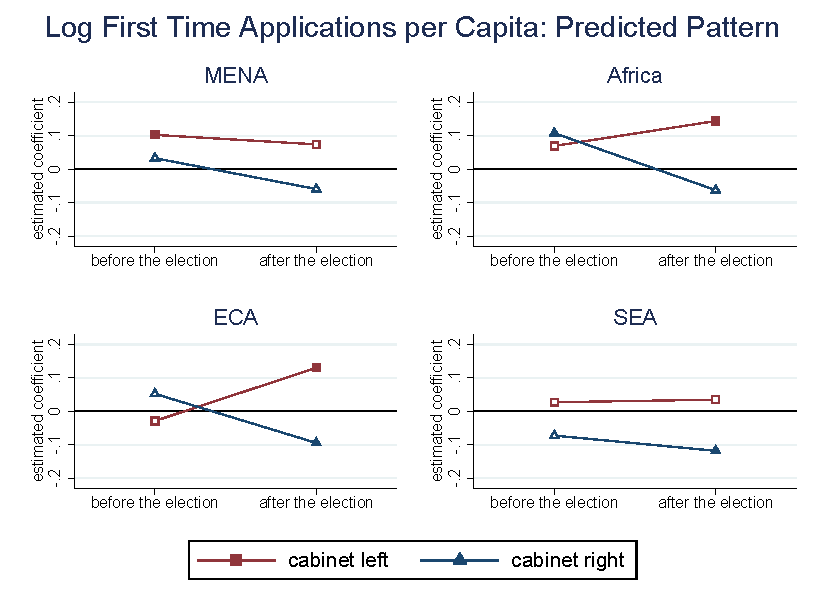
\includegraphics[width=0.8\textwidth]{figures_edited/app_graph1_by_region.pdf}
	\caption{log First Time Asylum Applications per Capita: Predicted Pattern}
\end{figure}

\begin{table}[!ht]\centering
	\footnotesize
	\renewcommand{\arraystretch}{1.1}
	\def\sym#1{\ifmmode^{#1}\else\(^{#1}\)\fi}
	\caption{log First-Time Asylum Applications per Capita: Predicted Pattern}
	\begin{subtable}{.5\linewidth}
		\centering
		\caption{Middle East and North Africa}
		\begin{tabular}{l*{2}{c}}
			\hline\hline
			                    &\multicolumn{1}{c}{(1)}&\multicolumn{1}{c}{(2)}\\
                    &\multicolumn{1}{c}{left}&\multicolumn{1}{c}{right}\\
\hline
before              &       0.103\sym{*}  &      0.0330         \\
                    &    (0.0492)         &    (0.0565)         \\
after               &      0.0742         &     -0.0594         \\
                    &    (0.0379)         &    (0.0487)         \\
\hline
Observations        &        4536         &        4536         \\

			\hline\hline
			\multicolumn{3}{c}{\footnotesize Standard errors in parentheses} \\
			\multicolumn{3}{c}{\footnotesize (\sym{*} \(p<0.05\), \sym{**} \(p<0.01\), \sym{***} \(p<0.001\))}\\
		\end{tabular}
	\end{subtable}%
	\begin{subtable}{.5\linewidth}
		\centering
		\caption{Africa}
		\begin{tabular}{l*{2}{c}}
			\hline\hline
			                    &\multicolumn{1}{c}{(1)}&\multicolumn{1}{c}{(2)}\\
                    &\multicolumn{1}{c}{left}&\multicolumn{1}{c}{right}\\
\hline
before              &      0.0696         &       0.108\sym{***}\\
                    &    (0.0423)         &    (0.0297)         \\
after               &       0.144\sym{**} &     -0.0627         \\
                    &    (0.0454)         &    (0.0429)         \\
\hline
Observations        &        7319         &        7319         \\

			\hline\hline
			\multicolumn{3}{c}{\footnotesize Standard errors in parentheses} \\
			\multicolumn{3}{c}{\footnotesize (\sym{*} \(p<0.05\), \sym{**} \(p<0.01\), \sym{***} \(p<0.001\))}\\
		\end{tabular}
	\end{subtable}%
\end{table}

\begin{table}[!ht]\centering
	\footnotesize
	\renewcommand{\arraystretch}{1.1}
	\def\sym#1{\ifmmode^{#1}\else\(^{#1}\)\fi}
	\caption{log First-Time Asylum Applications per Capita: Predicted Pattern}
	\begin{subtable}{.5\linewidth}
		\centering
		\caption{Europe and Central Asia}
		\begin{tabular}{l*{2}{c}}
			\hline\hline
			                    &\multicolumn{1}{c}{(1)}&\multicolumn{1}{c}{(2)}\\
                    &\multicolumn{1}{c}{left}&\multicolumn{1}{c}{right}\\
\hline
before              &     -0.0289         &      0.0523         \\
                    &    (0.0617)         &    (0.0377)         \\
after               &       0.130\sym{**} &     -0.0945\sym{*}  \\
                    &    (0.0419)         &    (0.0421)         \\
\hline
Observations        &        7365         &        7365         \\

			\hline\hline
			\multicolumn{3}{c}{\footnotesize Standard errors in parentheses} \\
			\multicolumn{3}{c}{\footnotesize (\sym{*} \(p<0.05\), \sym{**} \(p<0.01\), \sym{***} \(p<0.001\))}\\
		\end{tabular}
	\end{subtable}%
	\begin{subtable}{.5\linewidth}
		\centering
		\caption{South and East Asia}
		\begin{tabular}{l*{2}{c}}
			\hline\hline
			                    &\multicolumn{1}{c}{(1)}&\multicolumn{1}{c}{(2)}\\
                    &\multicolumn{1}{c}{left}&\multicolumn{1}{c}{right}\\
\hline
before              &      0.0271         &     -0.0726         \\
                    &    (0.0897)         &    (0.0440)         \\
after               &      0.0347         &      -0.118\sym{***}\\
                    &    (0.0352)         &    (0.0348)         \\
\hline
Observations        &        4696         &        4696         \\

			\hline\hline
			\multicolumn{3}{c}{\footnotesize Standard errors in parentheses} \\
			\multicolumn{3}{c}{\footnotesize (\sym{*} \(p<0.05\), \sym{**} \(p<0.01\), \sym{***} \(p<0.001\))}\\
		\end{tabular}
	\end{subtable}%
\end{table}

\clearpage
\textbf{Baseline Specification - Model 2}

\begin{figure}[!ht]
	\centering
	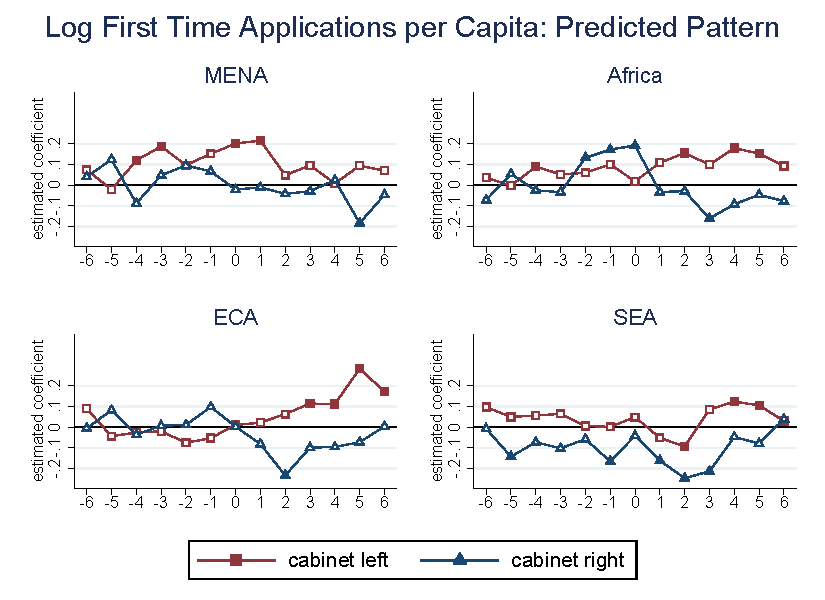
\includegraphics[width=0.7\textwidth]{figures_edited/app_graph2_by_region.pdf}
	\caption{log First Time Asylum Applications per Capita: Predicted Pattern}
\end{figure}

\begin{table}[!ht]\centering
	\footnotesize
	\renewcommand{\arraystretch}{1.1}
	\def\sym#1{\ifmmode^{#1}\else\(^{#1}\)\fi}
	\caption{log First-Time Asylum Applications per Capita: Predicted Pattern}
	\begin{subtable}{.5\linewidth}
	\centering
	\caption{Middle East and North Africa}
	\begin{tabular}{l*{2}{c}}
		\hline\hline
		                    &\multicolumn{1}{c}{(1)}&\multicolumn{1}{c}{(2)}\\
                    &\multicolumn{1}{c}{left}&\multicolumn{1}{c}{right}\\
\hline
 6 quarters before the election&      0.0815         &       0.110         \\
                    &     (0.113)         &    (0.0817)         \\
 5 quarters before the election&     -0.0251         &       0.161\sym{*}  \\
                    &     (0.116)         &    (0.0816)         \\
 4 quarters before the election&      0.0978         &     -0.0582         \\
                    &    (0.0704)         &     (0.105)         \\
 3 quarters before the election&       0.180\sym{**} &      0.0547         \\
                    &    (0.0665)         &    (0.0836)         \\
 2 quarters before the election&      0.0910         &       0.100         \\
                    &    (0.0523)         &    (0.0945)         \\
 1 quarters before the election&       0.155         &      0.0731         \\
                    &    (0.0987)         &    (0.0555)         \\
Quarter of the election&       0.206\sym{***}&     -0.0160         \\
                    &    (0.0522)         &    (0.0472)         \\
 1 quarters after the election&       0.219\sym{*}  &    -0.00495         \\
                    &    (0.0982)         &    (0.0952)         \\
 2 quarters after the election&      0.0557         &     -0.0362         \\
                    &    (0.0516)         &    (0.0828)         \\
 3 quarters after the election&       0.102         &     -0.0213         \\
                    &    (0.0719)         &    (0.0867)         \\
 4 quarters after the election&      0.0131         &      0.0303         \\
                    &    (0.0581)         &    (0.0753)         \\
 5 quarters after the election&      0.0981         &      -0.177\sym{*}  \\
                    &    (0.0508)         &    (0.0771)         \\
 6 quarters after the election&      0.0700         &     -0.0404         \\
                    &    (0.0853)         &    (0.0785)         \\
\hline
Observations        &        4536         &        4536         \\

		\hline\hline
		\multicolumn{3}{c}{\footnotesize Standard errors in parentheses} \\
		\multicolumn{3}{c}{\footnotesize (\sym{*} \(p<0.05\), \sym{**} \(p<0.01\), \sym{***} \(p<0.001\))}\\
	\end{tabular}
	\end{subtable}%
	\begin{subtable}{.5\linewidth}
	\centering
	\caption{Africa}
	\begin{tabular}{l*{2}{c}}
		\hline\hline
		                    &\multicolumn{1}{c}{(1)}&\multicolumn{1}{c}{(2)}\\
                    &\multicolumn{1}{c}{left}&\multicolumn{1}{c}{right}\\
\hline
 6 quarters before the election&      0.0582         &    -0.00310         \\
                    &    (0.0668)         &    (0.0509)         \\
 5 quarters before the election&      0.0365         &      0.0780         \\
                    &    (0.0520)         &    (0.0500)         \\
 4 quarters before the election&       0.126\sym{*}  &      0.0101         \\
                    &    (0.0551)         &    (0.0638)         \\
 3 quarters before the election&      0.0713         &   -0.000627         \\
                    &    (0.0670)         &    (0.0544)         \\
 2 quarters before the election&      0.0865         &       0.158\sym{*}  \\
                    &    (0.0516)         &    (0.0618)         \\
 1 quarters before the election&       0.100         &       0.182\sym{**} \\
                    &    (0.0548)         &    (0.0566)         \\
Quarter of the election&      0.0363         &       0.200\sym{***}\\
                    &    (0.0546)         &    (0.0512)         \\
 1 quarters after the election&       0.122         &     -0.0398         \\
                    &    (0.0665)         &    (0.0488)         \\
 2 quarters after the election&       0.171\sym{**} &    -0.00640         \\
                    &    (0.0565)         &    (0.0522)         \\
 3 quarters after the election&       0.109         &      -0.165\sym{**} \\
                    &    (0.0699)         &    (0.0633)         \\
 4 quarters after the election&       0.204\sym{***}&     -0.0565         \\
                    &    (0.0565)         &    (0.0720)         \\
 5 quarters after the election&       0.179\sym{**} &     -0.0329         \\
                    &    (0.0579)         &    (0.0720)         \\
 6 quarters after the election&       0.108         &     -0.0538         \\
                    &    (0.0559)         &    (0.0705)         \\
\hline
Observations        &        7319         &        7319         \\

		\hline\hline
		\multicolumn{3}{c}{\footnotesize Standard errors in parentheses} \\
		\multicolumn{3}{c}{\footnotesize (\sym{*} \(p<0.05\), \sym{**} \(p<0.01\), \sym{***} \(p<0.001\))}\\
	\end{tabular}
	\end{subtable}%
\end{table}

\begin{table}[!ht]\centering
	\footnotesize
	\renewcommand{\arraystretch}{1.1}
	\def\sym#1{\ifmmode^{#1}\else\(^{#1}\)\fi}
	\caption{log First-Time Asylum Applications per Capita: Predicted Pattern}
	\begin{subtable}{.5\linewidth}
		\centering
		\caption{Europe and Central Asia}
		\begin{tabular}{l*{2}{c}}
			\hline\hline
			                    &\multicolumn{1}{c}{(1)}&\multicolumn{1}{c}{(2)}\\
                    &\multicolumn{1}{c}{left}&\multicolumn{1}{c}{right}\\
\hline
 6 quarters before the election&      0.0431         &      0.0941         \\
                    &    (0.0790)         &    (0.0951)         \\
 5 quarters before the election&     -0.0538         &       0.149\sym{**} \\
                    &    (0.0774)         &    (0.0501)         \\
 4 quarters before the election&    -0.00855         &      0.0401         \\
                    &    (0.0724)         &    (0.0652)         \\
 3 quarters before the election&     0.00614         &      0.0228         \\
                    &    (0.0847)         &    (0.0418)         \\
 2 quarters before the election&     -0.0499         &      0.0263         \\
                    &    (0.0752)         &    (0.0696)         \\
 1 quarters before the election&     -0.0417         &       0.116         \\
                    &    (0.0791)         &    (0.0629)         \\
Quarter of the election&      0.0237         &      0.0185         \\
                    &    (0.0771)         &    (0.0756)         \\
 1 quarters after the election&      0.0362         &     -0.0659         \\
                    &    (0.0826)         &    (0.0452)         \\
 2 quarters after the election&      0.0781         &      -0.216\sym{***}\\
                    &    (0.0617)         &    (0.0639)         \\
 3 quarters after the election&       0.128\sym{*}  &     -0.0799         \\
                    &    (0.0542)         &    (0.0694)         \\
 4 quarters after the election&       0.123\sym{*}  &     -0.0793         \\
                    &    (0.0483)         &    (0.0664)         \\
 5 quarters after the election&       0.293\sym{***}&     -0.0556         \\
                    &    (0.0481)         &    (0.0639)         \\
 6 quarters after the election&       0.180\sym{***}&      0.0178         \\
                    &    (0.0401)         &    (0.0447)         \\
\hline
Observations        &        7365         &        7365         \\

			\hline\hline
			\multicolumn{3}{c}{\footnotesize Standard errors in parentheses} \\
			\multicolumn{3}{c}{\footnotesize (\sym{*} \(p<0.05\), \sym{**} \(p<0.01\), \sym{***} \(p<0.001\))}\\
		\end{tabular}
	\end{subtable}%
	\begin{subtable}{.5\linewidth}
		\centering
		\caption{South and East Asia}
		\begin{tabular}{l*{2}{c}}
			\hline\hline
			                    &\multicolumn{1}{c}{(1)}&\multicolumn{1}{c}{(2)}\\
                    &\multicolumn{1}{c}{left}&\multicolumn{1}{c}{right}\\
\hline
 6 quarters before the election&      0.0890         &      0.0825         \\
                    &    (0.0753)         &     (0.101)         \\
 5 quarters before the election&      0.0761         &     -0.0445         \\
                    &    (0.0995)         &    (0.0652)         \\
 4 quarters before the election&      0.0369         &    -0.00956         \\
                    &     (0.136)         &    (0.0735)         \\
 3 quarters before the election&      0.0529         &     -0.0880         \\
                    &     (0.126)         &    (0.0753)         \\
 2 quarters before the election&     0.00314         &     -0.0423         \\
                    &    (0.0944)         &    (0.0670)         \\
 1 quarters before the election&      0.0109         &      -0.149\sym{***}\\
                    &     (0.107)         &    (0.0433)         \\
Quarter of the election&      0.0577         &     -0.0258         \\
                    &     (0.100)         &    (0.0789)         \\
 1 quarters after the election&     -0.0383         &      -0.147\sym{*}  \\
                    &    (0.0740)         &    (0.0623)         \\
 2 quarters after the election&     -0.0770\sym{*}  &      -0.229\sym{***}\\
                    &    (0.0390)         &    (0.0631)         \\
 3 quarters after the election&       0.101         &      -0.196\sym{**} \\
                    &    (0.0766)         &    (0.0672)         \\
 4 quarters after the election&       0.135\sym{*}  &     -0.0307         \\
                    &    (0.0535)         &    (0.0524)         \\
 5 quarters after the election&       0.115\sym{***}&     -0.0606         \\
                    &    (0.0298)         &    (0.0475)         \\
 6 quarters after the election&      0.0367         &      0.0541         \\
                    &    (0.0695)         &    (0.0582)         \\
\hline
Observations        &        4696         &        4696         \\

			\hline\hline
			\multicolumn{3}{c}{\footnotesize Standard errors in parentheses} \\
			\multicolumn{3}{c}{\footnotesize (\sym{*} \(p<0.05\), \sym{**} \(p<0.01\), \sym{***} \(p<0.001\))}\\
		\end{tabular}
	\end{subtable}%
\end{table}

\end{document}